\documentclass[11pt,reqno]{amsart}

\usepackage{amsmath,amssymb,amsthm,mathtools}
\usepackage{tikz}
\usetikzlibrary{shapes.geometric, positioning, arrows.meta, decorations.pathmorphing, patterns}
\usepackage{booktabs}
\usepackage[hidelinks]{hyperref}

\allowdisplaybreaks
\raggedbottom

\newtheorem{theorem}{Theorem}[section]
\newtheorem{proposition}[theorem]{Proposition}
\newtheorem{lemma}[theorem]{Lemma}
\newtheorem{corollary}[theorem]{Corollary}
\theoremstyle{definition}
\newtheorem{definition}[theorem]{Definition}
\newtheorem{example}[theorem]{Example}
\newtheorem{warning}[theorem]{Warning}
\newtheorem{openproblem}[theorem]{Open Problem}
\theoremstyle{remark}
\newtheorem{remark}[theorem]{Remark}

\newcommand{\C}{\mathbb C}
\newcommand{\Z}{\mathbb Z}
\newcommand{\Chat}{\widehat{\mathbb C}}
\newcommand{\Fill}{\operatorname{Fill}}
\newcommand{\Exp}{\operatorname{Exp}}
\newcommand{\Int}{\operatorname{int}}
\newcommand{\dist}{\operatorname{dist}}
\newcommand{\id}{\operatorname{id}}
\newcommand{\Om}{\Omega}
\newcommand{\Omfree}{\Omega_{\mathrm{free}}}

\title[Protected planar carriers]{Protected planar carriers and\\access-preserving connector criteria}
\author{Matthew Robert Wesney}
\date{Draft I of 2026-07-27}

\begin{document}

\begin{abstract}
We develop a finite planar theory for connecting pairwise disjoint full
continua while preserving specified prime-end accesses and avoiding a frozen
obstacle set.  A protected ribbon-routing certificate is realized by a compact
connected full carrier whose protected crosscut chains survive as prime-end
chains, remain distinct, and retain their cyclic order; no local connectivity
of the connected atoms is required.  The conceptual center is an exact
free-component criterion: a protected carrier exists precisely when one
component of the completely frozen free domain admits simultaneous singleton
ports to every required atom.  The slit lemma underlying the criterion is
stated and proved here in a corrected form, with the boundary-anchored slits
mapped into the closed domain and the free endpoints retained for routing.  A
sufficient augmented-packet criterion, based on the compacta form of Alexander
duality, converts the criterion into a source-checkable test; for a fixed
typed packet assignment, fullification is order independent, and merger,
localization, and port-loss defects are persistent under monotone enlargement.
A cellwise criterion gives a directly checkable sufficient condition.
Examples separate the individual-access and common-component conditions and
exhibit persistent post-fullification packet mergers, and we compare the
certificate formalism with the standard continuum-hull constructions it
replaces.  A final section develops the finite direct-decoration application:
inside the pullback compactification of a terminal primitive root, finitely
many selected decoration packets admit a protected regulated connector that
avoids every unselected finite pullback and every end fiber.  The results are
purely finite and planar: they do not construct the virtual carrier, Wave
horizon, analytic correspondence, or uniform incidence bounds required for
Mandelbrot local connectivity.
\end{abstract}

\maketitle
\tableofcontents

% ---- begin A:intro ----
% Cluster A: introduction
% Body-only LaTeX; preamble macros, cite keys, and cross-cluster labels per CONVENTIONS.md.

\section{Introduction}\label{sec:intro}

\subsection{The problem}\label{subsec:A-problem}

A recurring problem in complex dynamics is to connect a finite family of
dynamical continua while preserving selected accesses to their complements.
In renormalization theory the continua are small filled Julia sets or their
combinatorial stand-ins: the Douady--Hubbard theory of polynomial-like maps
produces them \cite{DH85}; the a~priori bounds of Kahn--Lyubich organize them
into decorated configurations whose limbs and accesses carry the analytic
estimates \cite{KL08}; Dudko's roadmap describes virtual Julia sets as
connected hulls of Cantor families of small Julia sets carrying a finite part
of the critical orbit \cite{Dud25}; and Kahn--Kapiamba--Lyubich work with a
Hubbard tree constructed inside the full dynamical carrier of a primitive
renormalization \cite{KKL26}.  In every one of these settings a proof needs,
at some stage, a single compact connected full continuum --- a
\emph{carrier} --- joining finitely many pairwise disjoint full continua
(\emph{atoms}, in the terminology of the source manuscript, fixed in
Section~\ref{sec:prelim}) inside a Jordan localization, avoiding a compact
forbidden set of obstacles and critical values, and, crucially, leaving
intact certain designated accesses: prime ends of the atoms through which
later curve-family, width, or landing arguments will read the picture.

Ordinary connectedness is far too weak a specification for this task,
because a connector chosen merely to connect can destroy the data that made
the connection worth having.  Three failure modes recur.  The connector, or
an excess set absorbed together with it, can \emph{absorb a protected side}:
the enlarged carrier swallows the collar through which a marked access was
to be read, and no curve in the new complement lands there from the marked
side any more.  It can \emph{identify two prime ends}: two designated
crosscut chains, distinct in the complement of the atom, can become
equivalent in the complement of the enlarged carrier, so that marked access
data collapses.  And it can \emph{create a separator}: a connector placed at
one stage can disconnect the free region needed at a later stage, and
monotone enlargement never undoes a separation.  All three failures are
invisible to the coarse bookkeeping --- homeomorphism types, degrees,
critical words --- that dynamical constructions usually carry, which is what
makes them dangerous.

\subsection{Main results}\label{subsec:A-results}

The first group of results makes the failures precise and shows that they
already occur in the simplest possible situations.
Theorem~\ref{thm:no-least} (manuscript Theorem~6.12) shows that there is no
least compact connected full continuum containing even the two-point package
$\{-1,1\}$: carrier selection by minimization is not merely inconvenient but
impossible, since minimal carriers abound while no least one exists.
Proposition~\ref{prop:access-collision} (manuscript Proposition~6.15)
exhibits a conformal, critical-value-free, degree-one branch of $z\mapsto
z^{2}$ in which the very first monotone absorption of pulled excess erases a
protected prime-end access, together with its conformally transported copy,
irreversibly.  Between them, the two obstructions close both naive routes: no
least hull exists to select, and a proposed hull cannot be blindly
completed.

The positive theory replaces hull selection by certification.  A
\emph{protected ribbon-routing certificate}
(Definition~\ref{def:certificate}; manuscript Definition~10.1) records, as
explicit data: the atoms; the frozen forbidden set; the protected accesses,
each presented as a prime-end crosscut chain with its selected sides,
truncated so that the terminal collars are pairwise disjoint; free-port arcs
attaching to each atom at a single free point; and an embedded ribbon
tree joining the ports, with its planar cyclic data declared.
Theorem~\ref{thm:realization} (manuscript Theorem~10.4) realizes every
certificate by an actual carrier: a compact connected full continuum,
compactly contained in the localization, containing the atoms, missing the
forbidden set, with singleton attachment traces at the atoms, in whose
complement every protected chain survives as a prime-end chain, the survival
assignment being injective and cyclic-order preserving.  No local
connectivity of any atom is assumed at any point: the hypothesis that such
constructions can never afford is never used.

The conceptual center of the paper is the exact criterion,
Theorem~\ref{thm:free-component} (manuscript Theorem~10.8).  Freeze, before
any connector is chosen, the complete finite future inventory --- atoms,
closed terminal protected collars, separated obstacles, critical-value
exclusions, and the localization-forbidden set --- call the union $Q$, and
let $\Omfree=U\setminus Q$ be the frozen free domain.  Then a protected
ribbon-routing certificate exists if and only if a single component of
$\Omfree$ admits simultaneous singleton ports to every required atom.
Moreover, the failure mode is monotone: if a first protected collar or
obstacle separates two required port classes, no further monotone connector
enlargement inside the localization can repair the failure.  The criterion
converts an existential search over embedded trees into a property of one
planar set fixed in advance, and it explains, in hindsight, the design of
the certificate: everything the future proof will read must be frozen into
$Q$ before routing begins, precisely so that the criterion quantifies over
nothing but $Q$.

The criterion is exact but not yet checkable from partial data, and the next
group of results addresses checkability.  Theorem~\ref{thm:common-domain}
(manuscript Theorem~10.11) gives a sufficient test in packet form: if the
frozen inventory can be assigned to finitely many pairwise disjoint full
continua --- augmented atoms and separated obstacles, each the filled hull of
a connected seed --- with one unprotected free port per original atom, then
the compacta form of Alexander duality forces the common complement to be
connected, producing the single free component that the exact criterion
demands.  Theorem~\ref{thm:audit} (manuscript Theorem~10.14) turns the
packet clauses into an audit for a fixed typed assignment: fullification is
independent of processing order; the clauses reduce to three verifiable
conditions (coverage of the frozen inventory by compact connected seeds;
pairwise disjoint completions compactly contained in the localization;
nonempty unprotected exposure locus for every original atom); and each
failure --- packet merger, localization escape, port loss --- is witnessed
by a certificate that persists under every monotone same-label enlargement.
Proposition~\ref{prop:cellwise} (manuscript Proposition~10.15) then gives
the most directly checkable sufficient condition: if the seeds sit in
pairwise disjoint closed Jordan cells, with one boundary-reaching
unprotected arc per atom, every packet clause follows.

The final substantive section applies the framework at full strength.  In
the direct-decoration setting --- a terminal primitive root continuum with
two disjoint univalent pullbacks generating a pullback compactification with
finite fibers and end fibers --- Theorem~\ref{thm:carrier} (manuscript
Theorem~10.45) produces, for any finite selection of decoration addresses
and finitely many protected root prime-end chains with proper total
impression, a protected regulated connector whose packet fullifications stay
inside pairwise disjoint gap cells, avoid every unselected finite fiber and
every end fiber, and preserve the transported prime ends together with their
cyclic order.  The application exercises every part of the machinery:
gap-cell isolation, packet replacement, impression ports, the audit, and the
realization theorem.

\subsection{What is new, and what is not}\label{subsec:A-honest}

The ingredients of the proofs are classical: the Janiszewski separation
theorem, Carath\'eodory's theory of prime ends, filled hulls, the Jordan and
Schoenflies extension theorems, and \v{C}ech cohomology with the compacta
form of Alexander duality.  Readers should not expect --- and will not
find --- a new theorem of classical planar topology.  The contribution is
the assembled certification framework: accesses protected explicitly, as
crosscut chains with selected sides, rather than implicitly, as intentions;
cyclic order carried as data and proved to survive; the complete future
inventory frozen before routing, so that existence becomes a property of one
planar set; typed packets whose completion is order-independent; and failure
certificates that are monotone-persistent, so that a negative answer is as
stable and as citable as a positive one.  In short, the paper contributes
proof technology for access-preserving planar connection, not a new fact
about the plane.  Section~\ref{sec:comparison} compares this technology in
detail with the standard continuum-hull constructions it is designed to
replace: least hulls, monotone absorption, regulated and Hubbard trees,
Moore-type monotone quotients, and the lamination-lift candidate.

\subsection{Relation to the source manuscript}\label{subsec:A-source}

All results are reproduced, with notational streamlining only, from the
author's research manuscript \cite{MWman}, and every reproduced statement
carries its manuscript number in its bracketed title.  There is exactly one
intentional mathematical divergence.  Manuscript Lemma~10.7, the slit lemma
underlying the exact criterion, is formally inconsistent as printed: its
slits are declared as maps into the open domain yet are required to take a
boundary value at one end, and the removal prescribed there also deletes the
free endpoints that the proof of manuscript Theorem~10.8 later joins inside
the complement.  Lemma~\ref{lem:slits} states and proves the repaired
form --- slits mapped into the closed domain, boundary-anchored, with only
the open slit interiors removed and the free tips retained for routing ---
and the proof of Theorem~\ref{thm:free-component} is rewritten accordingly.
Remark~\ref{rem:repair} records the divergence precisely.  No other
statement has been altered.  The comparison Section~\ref{sec:comparison} and
the worked examples of Sections~\ref{sec:criterion} and~\ref{sec:audit} are
new expository material for this paper; they promote no manuscript claim.

\subsection{Organization}\label{subsec:A-roadmap}

Section~\ref{sec:prelim} fixes notation and collects the classical
background: full continua and filled hulls, Janiszewski's theorem, prime
ends and crosscut chains with their selected sides, the compacta form of
Alexander duality, and the Jordan--Schoenflies extension package, together
with the manuscript's terms \emph{atom} and \emph{fullification}.
Section~\ref{sec:obstructions} proves the two motivating obstructions,
Theorem~\ref{thm:no-least} and Proposition~\ref{prop:access-collision}.
Section~\ref{sec:comparison} carries out the comparison with standard
continuum-hull constructions.  Section~\ref{sec:certificates} defines
protected ribbon-routing certificates and proves the realization theorem and
its conformal naturality.  Section~\ref{sec:criterion} proves the repaired
slit lemma and the exact free-component criterion, together with an example
separating individual access from the existence of a common free component.
Section~\ref{sec:packets} develops augmented-atom packets and the
common-domain theorem, and Section~\ref{sec:audit} proves order-independent
fullification, the port audit with its persistent failure certificates, and
the cellwise criterion, together with an example of a persistent
post-fullification packet merger.  Section~\ref{sec:decoration} develops the
finite direct-decoration application, culminating in
Theorem~\ref{thm:carrier}.  Section~\ref{sec:scope} states the scope
boundary.

\subsection{Scope}\label{subsec:A-scope}

A firm boundary is maintained throughout, following the source manuscript's
own discipline (Warning~10.59 of \cite{MWman}).  This paper works entirely
with finite, explicitly given planar data.  It does not construct a virtual
carrier or virtual component package; it does not construct or use a Wave
horizon; it establishes no analytic correspondence and no covering or
immersion action; it proves no uniform incidence bound and no compression;
and it makes no claim about local connectivity of the Mandelbrot set.  The
open problems of the source manuscript that would supply such objects --- in
particular manuscript Open Problems~10.6 and~10.58 --- are cited only as
open, and nothing here advances them.  What is proved is exactly this: once
a finite protected certificate or packet system is supplied, the planar
realization problem is completely solved, with an exact criterion, checkable
sufficient conditions, and persistent failure certificates.
Section~\ref{sec:scope} restates the boundary in detail.
% ---- end A:intro ----

% ---- begin A:preliminaries ----
% Cluster A: notation and classical background
% Body-only LaTeX; preamble macros, cite keys, and cross-cluster labels per CONVENTIONS.md.

\section{Notation and classical background}\label{sec:prelim}

Everything in this section is classical.  It is collected once, in the
normalized forms used by the rest of the paper, for three reasons: the
statements are invoked repeatedly and in exact form; two of them --- the
compacta form of Alexander duality and the tameness of plane arcs --- are
easy to quote in weaker versions that would not support the proofs; and the
source manuscript's terminology --- \emph{atom}, \emph{package},
\emph{carrier}, \emph{fullification}, \emph{protected access},
\emph{collar} --- is fixed here at first use.

\subsection{Plane, sphere, and general notation}\label{subsec:A-notation}

Throughout, $\C$ is the complex plane, $\Z$ the integers, and
$\Chat=\C\cup\{\infty\}$ the Riemann sphere, identified with the round
sphere $S^2$ by stereographic projection and carrying its standard
orientation.  Compact subsets of $\C$ are exactly the compact subsets of
$\Chat$ missing $\infty$, and we pass between the two ambient spaces
without comment.  The symbol $\dist$ denotes Euclidean distance in $\C$;
diameters of crosscuts (Section~\ref{subsec:A-primeends}) are measured in
the spherical metric, and all other metric quantities are Euclidean.  For
a set $X$, $\Int X$ is its interior, $\partial X$ its boundary, and
$\overline{X}$ its closure, taken in the ambient space clear from context;
the relative closure of $X$ in a subspace $Y$ is written
$\overline{X}^{\,Y}$, as in the attachment trace \eqref{eq:B-trace}.

For sets $A,B$ we write $A\Subset B$, and say $A$ is \emph{compactly
contained} in $B$, if $\overline{A}$ is compact and
$\overline{A}\subset\Int B$; this is the manuscript's relation~$\Subset$.
A \emph{domain} is a nonempty connected open subset of $\C$ or $\Chat$; a
\emph{plane domain} is a domain in $\C$.  Every plane domain is polygonally
connected: any two of its points are joined by a polygonal path inside it
\cite{New51}.  A \emph{Jordan curve} is a homeomorphic image of the circle,
a \emph{Jordan arc} a homeomorphic image of $[0,1]$, and an \emph{open
Jordan arc} a Jordan arc with its two endpoints removed.  A \emph{Jordan
disk} (synonymously, a \emph{Jordan domain}) is a bounded plane domain
whose boundary is a Jordan curve; by the Jordan and Schoenflies theorems
recalled in Proposition~\ref{prop:A-extension} below, a Jordan disk is
simply connected, and its closure --- a \emph{closed Jordan disk} --- is
homeomorphic to the closed unit disk.  A \emph{continuum} is a nonempty
compact connected subset of $\C$ or $\Chat$; it is \emph{nondegenerate} if
it contains more than one point.

\subsection{Full continua, filled hulls, and fullification}
\label{subsec:A-full}

A compact set $K\subset\C$ is \emph{full} if $\C\setminus K$ is connected.
Following the source manuscript (equation~(9.5) of \cite{MWman}), the
\emph{filled hull} of a compact set $K\subset\C$ is
\begin{equation}\label{eq:A-fill}
\Fill(K)\;=\;K\,\cup\,
\bigcup\bigl\{\,B : B \text{ a bounded component of }\C\setminus K\,\bigr\},
\end{equation}
that is, $K$ together with the bounded components of its complement.  The
passage from $K$ to $\Fill(K)$ is called \emph{fullification}; the term is
the manuscript's, and it is used as a noun for the operation and,
occasionally, for its result.  The following properties are used
constantly and are recorded with proof.

\begin{lemma}[Basic properties of filled hulls]\label{lem:A-full}
Let $K\subset\C$ be compact, and let $\Omega_\infty(K)$ denote the
unbounded component of $\C\setminus K$.
\begin{enumerate}
\item $\Fill(K)=\C\setminus\Omega_\infty(K)$; in particular $\Fill(K)$ is
compact, and it is contained in every closed disk containing $K$.
\item The following are equivalent: $K$ is full; $\Chat\setminus K$ is
connected; $\Fill(K)=K$.
\item If $K$ is a continuum, then $\Fill(K)$ is a full continuum, and
$\Chat\setminus\Fill(K)=\Omega_\infty(K)\cup\{\infty\}$ is a simply
connected domain containing $\infty$.
\item The operator $\Fill$ is extensive ($K\subset\Fill(K)$), monotone
($K\subset L$ implies $\Fill(K)\subset\Fill(L)$), and idempotent
($\Fill(\Fill(K))=\Fill(K)$).
\end{enumerate}
\end{lemma}

\begin{proof}
(1) The set $\C\setminus\Omega_\infty(K)$ consists of $K$ together with
all bounded components of $\C\setminus K$, which is \eqref{eq:A-fill}; it
is closed because $\Omega_\infty(K)$ is open.  If $E$ is a closed disk with
$K\subset E$, then $\C\setminus E$ is a connected unbounded subset of
$\C\setminus K$, hence contained in $\Omega_\infty(K)$; taking complements
gives $\Fill(K)\subset E$.  Thus $\Fill(K)$ is closed and
bounded.

(2) The components of $\Chat\setminus K$ are the bounded components of
$\C\setminus K$ together with $\Omega_\infty(K)\cup\{\infty\}$: the latter
set is open in $\Chat$ (a spherical neighborhood of $\infty$ misses the
compact set $K$, and its intersection with $\C$, being connected and
unbounded, lies in $\Omega_\infty(K)$), it is connected, and its
complement within $\Chat\setminus K$ is the union of the bounded
components, which is open.
Hence $\Chat\setminus K$ is connected exactly when there are no bounded
components, which is fullness of $K$, which by \eqref{eq:A-fill} is the
identity $\Fill(K)=K$.

(3) Let $K$ be a continuum and let $B$ be a bounded component of
$\C\setminus K$.  The boundary of $B$ is contained in $K$: if a boundary
point $x$ of $B$ lay in $\C\setminus K$, its component $B'$ in
$\C\setminus K$ would be an open set containing $x$, hence meeting $B$,
hence equal to $B$; but then $x\in B$, contradicting openness of $B$ at
its own boundary point.  So $\partial B\subset K$.  Thus $\overline{B}=B\cup\partial B$ is a
connected set meeting $K$, and
$\Fill(K)=K\cup\bigcup_B\overline{B}$ is a union of connected sets each
meeting the connected set $K$, hence connected.  With (1) this makes
$\Fill(K)$ a continuum, and its complement in $\Chat$ is the domain
$\Omega_\infty(K)\cup\{\infty\}$, so $\Fill(K)$ is full.  Finally, a
domain in $\Chat$ whose complement is connected is simply connected
\cite{New51,Why42}, and the complement of the domain
$\Omega_\infty(K)\cup\{\infty\}$ is the continuum $\Fill(K)$.

(4) Extensivity is \eqref{eq:A-fill}.  For monotonicity, let
$K\subset L$; then $\Omega_\infty(L)$ is a connected unbounded subset of
$\C\setminus K$, hence $\Omega_\infty(L)\subset\Omega_\infty(K)$, and
taking complements in (1) gives $\Fill(K)\subset\Fill(L)$.  For
idempotence, the complement of $\Fill(K)$ is the single unbounded
component $\Omega_\infty(K)$, so $\Fill(\Fill(K))=\C\setminus
\Omega_\infty(K)=\Fill(K)$.
\end{proof}

The deeper absorption law
$\Fill(\Fill(K)\cup L)=\Fill(K\cup L)$, which makes fullification of a
typed packet independent of processing order, is
Lemma~\ref{lem:fill-absorption} below (manuscript Lemma~10.12); it is a
formal consequence of the three properties in clause~(4).

\begin{definition}[Package, atoms, carrier, fullification]
\label{def:A-package}
A \emph{package} is a finite union $S=A_1\cup\dots\cup A_s$ of pairwise
disjoint full continua, called its \emph{atoms}.  Atoms may be
degenerate: in Theorem~\ref{thm:no-least} the package consists of the two
points $\pm1$.  A \emph{carrier} of the package $S$ is a compact
connected full continuum $H\subset\C$ with $S\subset H$.  Both
\emph{atom} --- a required full continuum of the package --- and
\emph{fullification} --- the passage \eqref{eq:A-fill} --- are the source
manuscript's terms \cite{MWman} and are used in its sense throughout.
\end{definition}

\subsection{Janiszewski's separation theorem}\label{subsec:A-janiszewski}

A closed set $F\subset\Chat$ \emph{separates} points
$p,q\in\Chat\setminus F$ if $p$ and $q$ lie in different components of
$\Chat\setminus F$; the set $F$ is \emph{nonseparating} if
$\Chat\setminus F$ is connected.  By Lemma~\ref{lem:A-full}(2), a compact
subset of $\C$ is nonseparating in $\Chat$ exactly when it is full; the
two words are used interchangeably for such sets.

\begin{theorem}[Janiszewski's separation theorem; see \cite{New51,Why42}]
\label{thm:A-janiszewski}
Let $F_1,F_2\subset\Chat$ be closed sets whose intersection
$F_1\cap F_2$ is connected and nonempty, and let
$p,q\in\Chat\setminus(F_1\cup F_2)$.  If neither $F_1$ nor $F_2$
separates $p$ from $q$, then $F_1\cup F_2$ does not separate $p$ from
$q$.
\end{theorem}

\begin{corollary}\label{cor:A-janiszewski}
If $F_1,F_2\subset\Chat$ are closed and nonseparating and
$F_1\cap F_2$ is connected and nonempty, then $F_1\cup F_2$ is
nonseparating.  In particular, the union of two full compact subsets of
$\C$ whose intersection is connected and nonempty is full.
\end{corollary}

\begin{proof}
Let $p,q\in\Chat\setminus(F_1\cup F_2)$.  Since $\Chat\setminus F_1$ is
connected, $F_1$ does not separate $p$ from $q$, and likewise for $F_2$.
By Theorem~\ref{thm:A-janiszewski}, $F_1\cup F_2$ does not separate $p$
from $q$.  As the pair was arbitrary, $\Chat\setminus(F_1\cup F_2)$ is
connected.  The final sentence follows from Lemma~\ref{lem:A-full}(2).
\end{proof}

This is the form used in the Janiszewski induction of
Lemma~\ref{lem:tree-full}, where the intersections are singletons.  The
complementary situation of finitely many pairwise \emph{disjoint} full
compacta, where the stated form of the theorem does not apply, is handled
cohomologically, by the duality of Section~\ref{subsec:A-duality} and the
nerve argument of Lemma~\ref{lem:packets} (manuscript Lemma~10.10).

\subsection{Prime ends, crosscut chains, and protected accesses}
\label{subsec:A-primeends}

Informally, an \emph{access} to a compact set $K$ is a way of reaching
$\partial K$ from the complement.  It can be presented by a landing arc,
as the access $p_0^{+}(m)$ of Proposition~\ref{prop:access-collision} is
presented by the vertical segment $m+it$; but landing presentations
presuppose that something lands, and for the arbitrary continua handled in
this paper no landing is available.  The presentation that requires
nothing is Carath\'eodory's theory of prime ends \cite{Pom92}, which we
now recall in the normalization used throughout.

Let $\Omega\subset\Chat$ be a simply connected domain whose complement
contains at least two points.  The standing example is
$\Omega=\Chat\setminus K$ for a nondegenerate full continuum $K$, in which
case $\Omega$ is a simply connected domain containing $\infty$ by
Lemma~\ref{lem:A-full}(3); Jordan disks are a second example.  A
\emph{crosscut} of $\Omega$ is an open Jordan arc $\gamma\subset\Omega$
whose closure $\overline{\gamma}$ is a Jordan arc with two distinct
endpoints on $\partial\Omega$.  A crosscut divides $\Omega$ into exactly
two components, each a simply connected domain having $\gamma$ on its
boundary \cite{Pom92}.

A \emph{crosscut chain} (or \emph{prime-end chain}; Pommerenke's null
chains \cite{Pom92}, in the following normalization) is a sequence
\[
\Gamma=(\gamma_n,D_n)_{n\ge1}
\]
in which the $\gamma_n$ are pairwise disjoint crosscuts of $\Omega$ whose
spherical diameters tend to zero, and $D_n$, the \emph{selected side} of
$\gamma_n$, is one of the two components of $\Omega\setminus\gamma_n$,
subject to the coherence condition $D_{n+1}\subset D_n$ for every $n$.
Coherence and disjointness together force $\gamma_{n+1}\subset D_n$:
the crosscut $\gamma_{n+1}$ lies on the boundary of
$D_{n+1}\subset D_n$, so it lies in
$\overline{D_n}\cap\Omega=D_n\cup\gamma_n$, and it misses $\gamma_n$.
The record of a chain thus contains strictly more than the crosscuts: it
contains, for every $n$, the declaration of the selected side, and it is
exactly this declaration that the certificates of
Section~\ref{sec:certificates} protect.  Two chains are
\emph{equivalent} if each eventually divides the other, that is, if every
selected domain of either chain contains all sufficiently deep selected
domains of the other.  An equivalence class is a \emph{prime end} of
$\Omega$.

Two classical facts about prime ends are used.  First, the
Carath\'eodory correspondence: an orientation-preserving Riemann map
$\psi\colon\{|z|<1\}\to\Omega$ induces a bijection between the points of
the unit circle and the prime ends of $\Omega$, under which radial limits
correspond to chains; see \cite[Chapter~2]{Pom92}.  Second, the
\emph{impression}
\[
I(\Gamma)\;=\;\bigcap_{n\ge1}\overline{D_n}
\]
(closures in $\Chat$) is a nonempty compact connected subset of
$\partial\Omega$ --- the intersection of a decreasing sequence of
nonempty compacta --- and depends only on the prime end of $\Gamma$, not
on the representing chain \cite{Pom92}.  The nested closures
$\overline{D_n}$ decrease \emph{to} the impression; this is the form in
which impressions enter Lemma~\ref{lem:impression-port}.

The prime ends of $\Omega$ carry a natural \emph{cyclic order}: the one
transported from the unit circle by the Carath\'eodory correspondence.
It is independent of the choice of Riemann map, since two
orientation-preserving Riemann maps differ by a disk automorphism, which
preserves the cyclic orientation of the circle.  For a finite family of
prime ends represented by chains with pairwise disjoint selected sides,
the cyclic order can be computed inside the domain, with no reference to
a uniformization: choose one sufficiently deep oriented crosscut from
each chain; the cyclic order of the prime ends is the separation order of
these pairwise disjoint crosscuts in $\Omega$.  The computation is
carried out carefully, by means of embedded triods, in the proof of
Lemma~\ref{lem:crosscut-survival}, and that formulation is the one shown
to be invariant under carrier enlargement.

\begin{definition}[Protected access; collar]\label{def:A-protected}
Let $A$ be a nondegenerate atom.  A \emph{protected access} to $A$ is a
distinguished prime-end crosscut chain
$\Gamma=(\gamma_n,D_n)_{n\ge1}$ of $\Chat\setminus A$, recorded together
with its selected sides.  The terminal selected domain $D_1$ is the
\emph{collar} of the access, and $D_1\setminus A$ is its \emph{collar
tail}.  When finitely many protected accesses appear together inside a
Jordan localization, they are \emph{truncated} --- an initial segment of
each chain is discarded and the indices shifted --- so that the terminal
collar tails are pairwise disjoint, lie in the localization, and miss the
forbidden set and the other atoms; Section~\ref{sec:certificates} records
this normalization as part of the certificate data.
\end{definition}

The adjective \emph{protected} names a discipline, not a topological
property: a protected access is one that every later construction is
forbidden to disturb, in the precise sense that no connector may enter
its collar tail (Definition~\ref{def:certificate}).  The reward for the
discipline is the survival theorem, Lemma~\ref{lem:crosscut-survival}:
the chain then persists verbatim, with the same crosscuts and the same
selected sides, as a prime-end chain of the enlarged complement.

\subsection{\v{C}ech cohomology and Alexander duality}
\label{subsec:A-duality}

For a compact set $K\subset S^2$, $\check H^*(K;\Z)$ denotes \v{C}ech
cohomology with integer coefficients.  Two of its properties are needed
\cite{Hat02}: continuity --- the \v{C}ech cohomology of $K$ is the direct
limit of the singular cohomology of the open neighborhoods of $K$, so
that every class and every relation is realized in some neighborhood ---
and the Mayer--Vietoris sequence for pairs of compact sets in $S^2$.
Both are used in the nerve computation of Lemma~\ref{lem:packets} and in
the second proof of Lemma~\ref{lem:tree-full}.  The duality statement is
the following.

\begin{theorem}[Alexander duality, compacta form;
{\cite[pp.~256--257]{Hat02}}]\label{thm:A-duality}
For every nonempty proper compact subset $K\subset S^2$,
\begin{equation}\label{eq:A-duality}
\widetilde H_0\bigl(S^2\setminus K;\Z\bigr)\;\cong\;\check H^1(K;\Z).
\end{equation}
\end{theorem}

This is equation~(9.6) of the manuscript \cite{MWman}.  Reading
\eqref{eq:A-duality} at the level of connectivity gives the dictionary
used throughout the paper: $S^2\setminus K$ is connected exactly when
$\check H^1(K;\Z)=0$, and hence, by Lemma~\ref{lem:A-full}(2), a compact
set $K\subset\C$ is full exactly when $\check H^1(K;\Z)=0$.
``Nonseparating'' and ``vanishing first \v{C}ech cohomology'' are
synonyms, and the two proofs of Lemma~\ref{lem:tree-full} translate one
into the other.

\begin{warning}\label{warn:A-cech}
The \v{C}ech form of \eqref{eq:A-duality}, valid for an arbitrary
nonempty proper compact $K\subset S^2$, is required; the locally
contractible special case, in which \v{C}ech and singular cohomology
agree \cite{Hat02}, is not sufficient.  The atoms of this paper are
arbitrary full continua --- in general not locally connected, hence not
locally contractible, and admitting no CW approximation compatible with
their embedding --- and for such compacta duality genuinely fails with
singular cohomology in place of \v{C}ech.  The standard example is the
Warsaw circle $W\subset\C$, the closed topologist's sine curve completed
by an arc: $W$ separates the plane, so
$\widetilde H_0(S^2\setminus W;\Z)\cong\Z$, and accordingly
$\check H^1(W;\Z)\cong\Z$; but $W$ is path connected with trivial
fundamental group --- no loop can traverse the accumulation segment ---
so its singular homology $H_1$ vanishes and its \emph{singular}
cohomology gives $H^1_{\mathrm{sing}}(W;\Z)=0$.  Every duality argument in this paper ---
Lemma~\ref{lem:tree-full} (second proof), Lemma~\ref{lem:packets},
Lemma~\ref{lem:nested-packets} --- is therefore carried out in \v{C}ech
cohomology, and the nerve and continuity properties invoked there are the
\v{C}ech ones.
\end{warning}

\subsection{Jordan, Schoenflies, and Carath\'eodory extensions}
\label{subsec:A-extension}

The naturality statements of this paper
(Proposition~\ref{prop:naturality}, the naturality clauses of
Theorem~\ref{thm:audit}) rest on a package of classical extension
theorems, collected here with the exact attributes used later.

\begin{proposition}[Extension package]\label{prop:A-extension}
\leavevmode
\begin{enumerate}
\item \textup{(Jordan; Schoenflies)}  Every Jordan curve
$J\subset\Chat$ divides $\Chat$ into exactly two components, each a
simply connected domain with boundary $J$, and the closure of each is
homeomorphic to the closed unit disk.  Moreover, every homeomorphism
between two Jordan curves in $\Chat$ extends to a homeomorphism of
$\Chat$.
\item \textup{(Tameness of plane arcs)}  For every Jordan arc
$\alpha\subset\C$ there is a homeomorphism of $\C$ carrying $\alpha$ onto
the straight segment $[0,1]\times\{0\}$.  In particular every Jordan arc
extends to a Jordan curve, and no arc separates the plane.
\item \textup{(Carath\'eodory extension)}  Every conformal homeomorphism
$\phi\colon U\to V$ of Jordan disks extends to a homeomorphism
$\overline{U}\to\overline{V}$ of their closures.
\item \textup{(Glued sphere extension)}  Every orientation-preserving
conformal homeomorphism $\phi\colon U\to V$ of Jordan disks
$U,V\subset\C$ extends to an orientation-preserving homeomorphism
$\Phi\colon\Chat\to\Chat$, and $\Phi$ may be chosen with
$\Phi(\infty)=\infty$.
\item \textup{(Fill-equivariance)}  Every homeomorphism $\Phi$ of
$\Chat$ with $\Phi(\infty)=\infty$ satisfies
$\Phi(\Fill(K))=\Fill(\Phi(K))$ for every compact $K\subset\C$.
\end{enumerate}
\end{proposition}

\begin{proof}
Clauses (1) and (2) are classical plane topology; see
\cite{New51,Why42}.  Clause (3) is Carath\'eodory's theorem on boundary
extension of Riemann maps of Jordan domains; see \cite{Pom92}.

For (4), extend $\phi$ to a homeomorphism
$\overline{\phi}\colon\overline{U}\to\overline{V}$ by (3).  Its boundary
restriction is a homeomorphism $\partial U\to\partial V$ of Jordan
curves; the complementary sets $\Chat\setminus U$ and $\Chat\setminus V$
are closed Jordan disks by (1), and a homeomorphism between the boundary
circles of two closed disks extends over the disks (cone the
homeomorphism off an interior point, after identifying each closed disk
with the standard one by (1)).  Gluing the two extensions along the
boundary curves yields a homeomorphism $\Phi\colon\Chat\to\Chat$ with
$\Phi|_U=\phi$.  A sphere homeomorphism that preserves orientation on a
nonempty open set preserves it globally, so $\Phi$ is orientation
preserving.  Finally, $\infty$ lies in the interior of the complementary
disk $\Chat\setminus U$, and $\Phi(\infty)$ in the interior of
$\Chat\setminus V$; composing $\Phi$ with a homeomorphism of the closed
disk $\Chat\setminus V$ that fixes $\partial V$ pointwise and carries
$\Phi(\infty)$ to $\infty$ (such a homeomorphism exists, interiors of
disks being homogeneous relative to the boundary), extended by the
identity on $\overline{V}$, arranges $\Phi(\infty)=\infty$ without
disturbing $\Phi|_U=\phi$.

For (5), the restriction $\Phi|_{\C}$ is a homeomorphism of $\C$ onto
itself.  It maps $\C\setminus K$ homeomorphically onto
$\C\setminus\Phi(K)$ and permutes complementary components.  A
homeomorphism of $\C$ is proper, so the image of the unbounded component
of $\C\setminus K$ is unbounded and the images of bounded components are
bounded; hence $\Phi(\Omega_\infty(K))=\Omega_\infty(\Phi(K))$, and
taking complements as in Lemma~\ref{lem:A-full}(1) gives
$\Phi(\Fill(K))=\Fill(\Phi(K))$.
\end{proof}

Clause (4) is the mechanism behind every naturality statement in the
paper: a univalent change of Jordan localization extends to a sphere
homeomorphism, and a sphere homeomorphism preserves all the notions the
certificates are built from --- compactness, connectedness, fullness (by
clause (5) and Lemma~\ref{lem:A-full}), crosscuts, selected sides, null
chains, intersections and disjointness, and, when orientation is
preserved, the cyclic order of prime ends and the ribbon structure of an
embedded tree.  Clause (2) is used in the slit-straightening steps of the
repaired slit lemma (Lemma~\ref{lem:slits}).

This completes the classical inventory.  The dynamical vocabulary of the
source manuscript --- frozen inventory, free domain, ports, packets,
audits --- is introduced where it is first needed:
the frozen free domain $\Omfree$ in Section~\ref{sec:criterion}, packets
and their audit in Sections~\ref{sec:packets} and~\ref{sec:audit}.
% ---- end A:preliminaries ----

% ---- begin B:obstructions ----
% Cluster B: motivating obstructions (manuscript Theorem 6.12, Section 6.4, Proposition 6.15)
% Body-only LaTeX; preamble macros and theorem environments per CONVENTIONS.md.

\section{Obstructions to naive carriers}\label{sec:obstructions}

Before any positive theory is developed, it is worth recording exactly why the
two most tempting shortcuts fail. The first shortcut is a \emph{selection}
rule: given the finite package of marked continua that a carrier must contain,
simply take the least compact connected full set containing it. The second is
a \emph{completion} rule: given a proposed carrier and the excess produced by
pulling it back through the dynamics, simply absorb that excess monotonically
until the process stabilizes. Both rules are natural, both are implicit in
informal uses of connected hulls, and both fail --- the first because the
minimizer does not exist, the second because absorption destroys precisely the
access data that a protected carrier is supposed to preserve. The two
obstructions below are taken from the source manuscript
\cite[Theorem~6.12, Proposition~6.15]{MWman}; they are elementary, but they
dictate the architecture of everything that follows, and in particular the
certificate formalism of Section~\ref{sec:certificates}. The comparison with
standard continuum-hull constructions in Section~\ref{sec:comparison} should
be read with both examples in mind.

\subsection{Failure of least carriers}\label{subsec:B-no-least}

Recall from Section~\ref{sec:prelim} that a compact set $K\subset\C$ is
\emph{full} if $\C\setminus K$ is connected, and that a \emph{carrier} for a
finite package $S\subset\C$ is a compact connected full continuum containing
$S$. Order the carriers of a fixed package by inclusion. A \emph{least}
carrier would be a carrier contained in every other carrier of the same
package. The following theorem shows that a least carrier fails to exist
already for the simplest nondegenerate package: two points, with the identity
map as dynamics and with no obstacle set whatsoever.

\begin{theorem}[No least connected full carrier; manuscript Theorem 6.12]\label{thm:no-least}
There is no least compact connected full plane continuum containing the
two-point package $S=\{-1,1\}$, even with identity dynamics and no obstacles.
\end{theorem}

\begin{proof}
Let
\[
A_+=\{e^{i\theta}:0\le\theta\le\pi\},
\qquad
A_-=\{e^{i\theta}:-\pi\le\theta\le 0\}
\]
be the upper and lower semicircles of the unit circle joining $-1$ to $1$.
Each is an arc, that is, a homeomorphic image of $[0,1]$; hence each is
compact and connected. An arc does not separate the plane
\cite{New51}, so $\C\setminus A_\pm$ is connected and each $A_\pm$ is full.
Each contains $S$, so each is a carrier for $S$; in particular the family of
carriers is nonempty. Finally, the semicircles meet exactly in their common
endpoints:
\[
A_+\cap A_-=S .
\]

Suppose a least carrier $H$ existed. By definition of leastness, $H$ is
contained in every carrier of $S$; applying this to the two carriers $A_+$
and $A_-$ gives
\[
H\subset A_+\cap A_-=S .
\]
On the other hand $S\subset H$, since $H$ is a carrier of the package $S$.
Hence $H=S=\{-1,1\}$. But the two-point set $S$ is disconnected, while a
carrier is by definition connected. This contradiction shows that no least
carrier exists.
\end{proof}

The failure is one of \emph{leastness}, not of minimality: minimal carriers
exist in abundance. Indeed, a subcontinuum of an arc that contains both
endpoints is the whole arc, so every arc from $-1$ to $1$ --- in particular
each of $A_+$ and $A_-$, and every circular arc through $-1$ and $1$ --- is a
minimal element of the family of carriers. The order-theoretic structure is
thus the worst possible for a canonical selection: a large family of pairwise
distinct minimal elements and no least one.

The moral drawn in the manuscript is the one that governs this paper: ``take
the minimal connected full hull'' is not a carrier rule. Even for two points
and trivial dynamics, the carrier is underdetermined, and the ambiguity is not
a set-theoretic accident but a genuine topological degree of freedom --- the
two semicircles pass on opposite sides of the origin, and in any configuration
with obstacles, additional atoms, or protected accesses, that choice of side
is visible to the rest of the construction. A regulated connector system,
together with its access or isotopy class and a forward-coherence proof, is
therefore \emph{additional data}, beyond anything determined by the package
itself. Recording that data explicitly, and saying precisely when it can be
realized by an actual carrier, is the task of the certificate formalism of
Section~\ref{sec:certificates}.

\begin{figure}[ht]
\centering
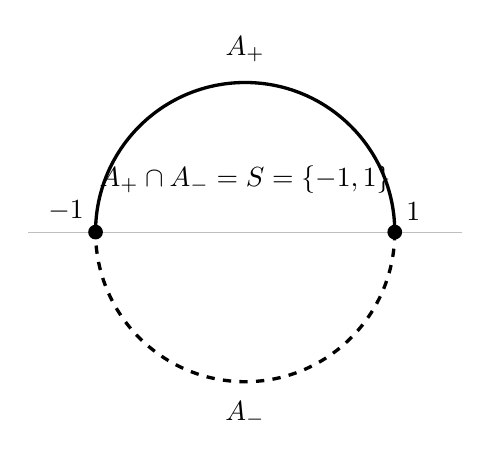
\begin{tikzpicture}[scale=1.9]
  % upper semicircle: solid carrier A_+
  \draw[very thick] (1,0) arc[start angle=0, end angle=180, radius=1];
  \node at (0,1.22) {$A_+$};
  % lower semicircle: dashed carrier A_-
  \draw[very thick, dashed] (1,0) arc[start angle=0, end angle=-180, radius=1];
  \node at (0,-1.22) {$A_-$};
  % faint horizontal axis for orientation
  \draw[gray!50] (-1.45,0) -- (1.45,0);
  % the package points
  \fill (-1,0) circle (1.4pt);
  \node[above left=1pt] at (-1,0) {$-1$};
  \fill (1,0) circle (1.4pt);
  \node[above right=1pt] at (1,0) {$1$};
  % annotation
  \node at (0,0.35) {$A_+\cap A_-=S=\{-1,1\}$};
\end{tikzpicture}
\caption{Two minimal carriers for the package $S=\{-1,1\}$: the upper
semicircle $A_+$ (solid) and the lower semicircle $A_-$ (dashed). Each is an
arc, hence a compact connected full continuum containing $S$, and they meet
only in the package points. A least carrier would be contained in their
intersection $S$, which is disconnected; hence no least carrier exists
(Theorem~\ref{thm:no-least}).}
\label{fig:no-least}
\end{figure}

\subsection{An analytic protected-access collision}\label{subsec:B-collision}

Theorem~\ref{thm:no-least} rules out selecting the carrier by minimization.
The remaining naive rule is completion: accept an arbitrary proposed carrier
and then absorb, monotonically, whatever excess the dynamics pulls back onto
it. The manuscript's Section~6.4 shows that this rule fails as well, and
fails in the most favorable analytic circumstances imaginable: a single
conformal, critical-value-free, degree-one branch of the quadratic map,
acting on an interval. The absorption step erases a protected prime-end
access, and monotonicity then propagates the erasure forever.

We reproduce the analytic setup exactly. Let
\[
f(z)=z^{2},\qquad I=[1,2],\qquad m=\tfrac32,
\]
and let
\begin{equation}\label{eq:B-Q}
Q=\Bigl\{\,z:\bigl|z-\tfrac32\bigr|\le\tfrac12,\ \operatorname{Im}z\ge 0\,\Bigr\}
\end{equation}
be the closed upper half-disk of radius $\tfrac12$ centered at $m$. Set
\[
U^{-}=\bigl\{z:\bigl|z-\tfrac32\bigr|<1\bigr\},
\qquad
U^{+}=f(U^{-}).
\]
The disk $U^{-}$ lies in the half-plane $\operatorname{Re}z>\tfrac12$. Two
consequences follow. First, $0\notin U^{-}$, so $f'(z)=2z\ne 0$ on $U^{-}$
and the critical point of $f$ is outside the domain; since $f(z)=f(w)$ forces
$w=\pm z$, and $U^{-}$ is disjoint from its antipode
$-U^{-}\subset\{\operatorname{Re}z<-\tfrac12\}$, the restriction
\begin{equation}\label{eq:B-branch}
F=f|_{U^{-}}:U^{-}\longrightarrow U^{+}
\end{equation}
is injective, hence a conformal homeomorphism onto $U^{+}$. Second, the
critical value $0=f(0)$ is not in $U^{+}$, so the branch is
critical-value-free. Take
\begin{equation}\label{eq:B-stages}
T_0=I,\qquad T_0'=Q,\qquad T_1=f(I)=[1,4],\qquad T_1'=f(Q).
\end{equation}
Within this branch the stage-$0$ data are the pullbacks of the stage-$1$
data:
\begin{equation}\label{eq:B-pullback}
T_0'=F^{-1}(T_1'),\qquad T_0=F^{-1}(T_1).
\end{equation}
Thus $T_0=I$ is the proposed carrier at stage $0$, and $T_0'=Q$ is the actual
pulled carrier: the completion rule under scrutiny would replace $T_0$ by an
enlargement absorbing the difference. Two pieces of terminology from the
manuscript's completion formalism are needed, and we define them at first
use. The \emph{pulled excess} at stage $0$ is the difference
$X_0=T_0'\setminus T_0$ between the pulled carrier and the proposed carrier.
The \emph{attachment trace} of the excess on the proposed carrier is
\begin{equation}\label{eq:B-trace}
\tau_{T_0}(X_0):=\overline{X_0}^{\,T_0'}\cap T_0,
\end{equation}
where $\overline{X_0}^{\,T_0'}$ denotes the closure of $X_0$ taken in the
actual pulled carrier $T_0'$: the trace records where the excess attaches to
the proposed carrier after closure, not where it meets it as a set.

\begin{proposition}[Quadratic protected-access collision; manuscript Proposition 6.15]\label{prop:access-collision}
In the setup \eqref{eq:B-Q}--\eqref{eq:B-pullback}, the pulled excess has the
single component
\[
X_0=Q\setminus I
\]
with attachment trace
\[
\tau_{T_0}(X_0)=\overline{X_0}^{\,T_0'}\cap T_0=I .
\]
The closure is taken in the actual pulled carrier $T_0'$; in particular, the
trace is not $X_0\cap T_0$, which is empty by the definition of the excess.
The complete one-stage itinerary of the excess is
\[
X_0\longmapsto f(X_0),
\]
on the right sheet with critical word $0$. If the upper access $p_0^{+}(m)$,
represented by the vertical segment $m+it$, is protected, then every monotone
attachment-complete enlargement absorbing $X_0$ erases that access and its
transported access $F_{*}p_0^{+}(m)$.
\end{proposition}

\begin{proof}
\emph{The excess and its trace.}
A point of $Q$ lies in $I=[1,2]$ exactly when it is real, so
\[
X_0=Q\setminus I
=\Bigl\{\,z:\bigl|z-\tfrac32\bigr|\le\tfrac12,\ \operatorname{Im}z>0\,\Bigr\}
\]
is the relative upper half-disk with its real diameter removed. It is the
intersection of the closed disk of radius $\tfrac12$ about $m$ with the open
upper half-plane, hence convex, hence connected: the excess has a single
component. Its closure in $\C$ is the entire closed half-disk
$Q$, since every point $x\in I$ is the limit of the points $x+it\in X_0$ as
$t\downarrow 0$. As $Q=T_0'$, the closure of $X_0$ in $T_0'$ is all of $Q$,
and therefore
\[
\tau_{T_0}(X_0)=\overline{X_0}^{\,T_0'}\cap T_0=Q\cap I=I:
\]
the excess attaches to the proposed carrier along the entire interval, even
though $X_0\cap T_0=\varnothing$ by construction. This is the reason the
completion formalism must work with attachment traces rather than
intersections: the naive intersection sees nothing, while the closure sees an
attachment along all of $I$.

\emph{The itinerary.}
Since $0\notin U^{-}$, we have $F'(z)=2z\ne 0$ throughout $U^{-}$, and the
selected branch avoids the critical value $0\notin U^{+}$. The itinerary of
the excess therefore consists of the single right-sheet, degree-one step
$X_0\mapsto f(X_0)$ with no critical encounter; its critical word is $0$.
There is no hidden multivalence, folding, or critical intrusion anywhere in
the example.

\emph{Erasure of the protected access.}
The access $p_0^{+}(m)$ is the access to $I$ at the interior point $m$ from
the upper side, represented by the curve $t\mapsto m+it$, $t\in(0,\epsilon]$,
which lies in $U^{-}\setminus I$ and lands at $m$. Suppose a monotone
attachment-complete enlargement absorbs $X_0$ while retaining $I$. The
enlarged carrier is compact and contains $X_0\cup I$; since it is closed and
$\overline{X_0}=Q$, it contains the entire half-disk $Q$. But $Q$ contains an
upper relative half-neighborhood of $m$: the set
\[
\Bigl\{\,z:\bigl|z-\tfrac32\bigr|<\tfrac12,\ \operatorname{Im}z\ge 0\,\Bigr\}
\subset Q
\]
is a neighborhood of $m$ in the closed upper half-plane. Consequently, any
curve in $U^{-}$ landing at $m$ from the upper side eventually lies in this
half-neighborhood, hence in $Q$, hence in the enlarged carrier. No curve in
the complement $U^{-}\setminus Q$ can therefore land at $m$ from the upper
side: the access $p_0^{+}(m)$ no longer exists as an access from the
complement of the enlarged carrier. Monotonicity makes the erasure permanent:
further monotone enlargement only adds points to the carrier and so cannot
restore a complement access through a set already absorbed.

\emph{Transport to stage $1$.}
The branch $F$ of \eqref{eq:B-branch} is a conformal homeomorphism of
$U^{-}$ onto $U^{+}$ carrying $I$ to $T_1=[1,4]$, $Q$ to $T_1'$, $X_0$ to the
stage-$1$ excess $T_1'\setminus T_1$, and the representing curve $m+it$ to a
curve in $U^{+}\setminus T_1$ landing at $f(m)=\tfrac94$ from the
$F$-selected side. A homeomorphism of the localization carries complement
curves to complement curves, so the same argument applied to the image data
erases the transported access $F_{*}p_0^{+}(m)$ at stage $1$. Conformality
thus transports the identical conclusion to stage $1$, as claimed.
\end{proof}

\begin{figure}[ht]
\centering
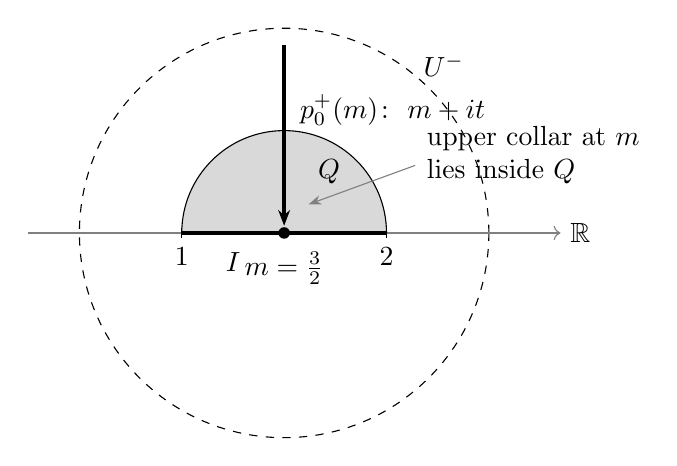
\begin{tikzpicture}[scale=2.6]
  % localization disk U^- (dashed)
  \draw[dashed] (1.5,0) circle[radius=1];
  \node at (2.28,0.82) {$U^{-}$};
  % real axis
  \draw[->,gray] (0.25,0) -- (2.85,0) node[right,black] {$\mathbb{R}$};
  % excess half-disk Q (shaded)
  \fill[gray!30] (2,0) arc[start angle=0, end angle=180, radius=0.5] -- cycle;
  \draw (2,0) arc[start angle=0, end angle=180, radius=0.5];
  \node at (1.72,0.3) {$Q$};
  % proposed carrier I = [1,2]
  \draw[very thick] (1,0) -- (2,0);
  \draw (1,0.025) -- (1,-0.025) node[below] {$1$};
  \draw (2,0.025) -- (2,-0.025) node[below] {$2$};
  \node[below] at (1.25,-0.05) {$I$};
  % marked point m
  \fill (1.5,0) circle (0.8pt);
  \node[below] at (1.5,-0.045) {$m=\tfrac32$};
  % protected access arrow from above, along m + it
  \draw[-{Stealth[length=2mm]},very thick] (1.5,0.92) -- (1.5,0.035);
  \node[right] at (1.53,0.6) {$p_0^{+}(m)\colon\ m+it$};
  % annotation: the collar at m is inside Q
  \node[align=left,right] at (2.15,0.38) {upper collar at $m$\\ lies inside $Q$};
  \draw[-{Stealth[length=1.6mm]},gray] (2.14,0.33) -- (1.62,0.14);
\end{tikzpicture}
\caption{The quadratic protected-access collision
(Proposition~\ref{prop:access-collision}). The proposed carrier is the
interval $I=[1,2]$ (thick); the pulled carrier is the closed upper half-disk
$Q$ (shaded) of radius $\tfrac12$ about $m=\tfrac32$, inside the localization
disk $U^{-}$ (dashed) on which $f(z)=z^{2}$ restricts to a conformal
homeomorphism. The protected upper access $p_0^{+}(m)$, represented by the
vertical segment $m+it$, must traverse $Q$: absorbing the excess
$X_0=Q\setminus I$ forces the carrier to contain the entire upper collar at
$m$ and erases the access.}
\label{fig:access-collision}
\end{figure}

\subsection{What the obstructions force}\label{subsec:B-moral}

The two obstructions are complementary and together close off every naive
route. Theorem~\ref{thm:no-least} shows that the carrier cannot be
\emph{selected} canonically: there is no least connected full hull, even for
two points with identity dynamics, so any construction that speaks of ``the''
minimal carrier is speaking of an object that does not exist.
Proposition~\ref{prop:access-collision} shows that the carrier cannot be
\emph{completed} blindly either: the very first monotone absorption of a
pulled excess can erase a protected prime-end access, and monotonicity then
makes the loss irreversible at every later stage of the enlargement, as well
as at the conformally transported stage.

The second obstruction is the sharper of the two, because of what it does
\emph{not} involve. In the manuscript's collision bookkeeping \cite{MWman},
which records sheet mergers, critical intrusions, obstacle collisions, access
identifications, and localization escapes in the order
$(\chi_{\mathrm{sheet}},\chi_{\mathrm{crit}},\chi_{\mathrm{obs}},
\chi_{\mathrm{access}},\chi_{\mathrm{loc}})$, the collision tuple of the
completed enlargement in this example is
\[
\bigl(\varnothing,\ \varnothing,\ \varnothing,\
\{p_0^{+}(m),\,F_{*}p_0^{+}(m)\},\ \varnothing\bigr):
\]
every coordinate vanishes except the access coordinate. The
branch is conformal, degree one, and critical-value-free; there is no sheet
merger, no obstacle, and no localization escape. Consequently no amount of
critical-point bookkeeping --- however carefully one tracks critical words,
critical values, or degrees --- can detect, let alone excuse, the collision.
Access protection is invisible to critical data and must be carried as
explicit data of its own, with its own survival theorem.

This is exactly what the remainder of the paper provides. The certificate
formalism of Section~\ref{sec:certificates} records the protected accesses as
prime-end crosscut chains \cite{Pom92} with pairwise disjoint terminal
collars, together with free-port arcs carrying singleton attachment traces
and a ribbon tree with declared sides; Theorem~\ref{thm:realization} then
realizes any such certificate by an actual compact connected full carrier in
which every protected chain survives with unchanged cyclic order. The
selection ambiguity of Theorem~\ref{thm:no-least} is resolved not by
minimization but by the certificate itself: the connector system, its access
class, and its routing are supplied as data, and the exact free-component
criterion of Section~\ref{sec:criterion} determines precisely when such data
can be supplied at all.
% ---- end B:obstructions ----

% ---- begin A:comparison ----
% Cluster A: comparison with standard continuum-hull constructions
% Review-required new expository material; promotes no manuscript claim.
% Body-only LaTeX; preamble macros, cite keys, and cross-cluster labels per CONVENTIONS.md.

\section{Comparison with standard continuum-hull constructions}
\label{sec:comparison}

The certificate formalism developed from Section~\ref{sec:certificates}
onward is offered as a replacement for a family of standard constructions,
and it is fair to ask what, exactly, is being replaced and why.  This
section compares the framework with the five constructions a practitioner
would reach for first: least or minimal connected full hulls; monotone
absorption of pulled excess; regulated and Hubbard trees in uniformized or
locally connected coordinates; Moore decompositions and monotone
quotients; and the lamination-lift candidate of the source manuscript.
The two obstructions of Section~\ref{sec:obstructions} already dispose of
the first two; the remaining three fail for structural reasons that are
worth stating precisely, because they explain several design decisions of
the certificate formalism that would otherwise look pedantic.  Throughout,
the comparison is with respect to the task fixed in the introduction:
join finitely many pairwise disjoint full atoms inside a Jordan
localization, avoid a frozen forbidden set, and \emph{preserve designated
prime-end accesses together with their cyclic order}.  Constructions that
solve a different problem well are not thereby criticized; the claim is
only that none of them solves this one, and that the last of them ---
the lamination lift --- is an open candidate, not a construction.

\subsection{Least and minimal connected full hulls}
\label{subsec:A-comp-least}

The most tempting rule is extremal: ``take the least connected full hull
of the required package.''  Theorem~\ref{thm:no-least} (manuscript
Theorem~6.12) shows the rule names no object, already for the two-point
package $S=\{-1,1\}$ with identity dynamics and no obstacles: the upper
and lower semicircles are carriers meeting exactly in $S$, so a least
carrier would be contained in their disconnected intersection.  The
failure is specific to \emph{leastness}: minimal carriers exist in
abundance --- every arc from $-1$ to $1$ is one --- and form a large
antichain.  An extremal selection principle therefore cannot even break
the tie between the two semicircles, and the tie is not innocent: the two
choices pass on opposite sides of the origin, and in any configuration
with obstacles or protected collars that choice of side is visible to
every later routing step.  The source manuscript sharpens the point
dynamically \cite[Proposition~6.11]{MWman}: a package, full connected
carriers, critical-value-free degree-one selected-carrier dynamics, and
identical coarse orbit labels are realized simultaneously by an interval
and by a triod, and attachment-freeness holds in only one of the two
models, so no data of the listed kinds can select between them.

The published connected-hull descriptions in the renormalization
literature are not at fault here, and the comparison should not be read
as a criticism of them.  Dudko's roadmap describes virtual Julia sets as
connected hulls of Cantor families of small Julia sets carrying a finite
part of the critical orbit \cite{Dud25}; that description specifies
\emph{which} continua a carrier must contain, and it does not purport to
specify \emph{how} they are joined.  Theorem~\ref{thm:no-least} shows
that the routing is genuinely additional data --- in the manuscript's
words, a regulated connector system, together with its access or isotopy
class and a forward-coherence proof, is additional data \cite{MWman} ---
and the certificate of Definition~\ref{def:certificate} is exactly a
format for that data, with Theorem~\ref{thm:free-component} deciding when
the format can be filled in at all.

\subsection{Monotone absorption of pulled excess}
\label{subsec:A-comp-absorption}

The second rule is completion: accept any proposed carrier and absorb,
monotonically, whatever excess the dynamics pulls back onto it, until the
process stabilizes.  Unlike the least hull, this rule is well defined:
the manuscript proves that the finite inflationary completion operator
stabilizes at a least fixed point, unique and conjugation-equivariant
\cite[Theorem~6.14]{MWman}.  The defect is not existence but what
completion destroys.  Proposition~\ref{prop:access-collision} (manuscript
Proposition~6.15) exhibits a conformal, critical-value-free, degree-one
branch of $z\mapsto z^2$ in which the very first absorption of pulled
excess --- the relative upper half-disk attaching to the interval along
its entire length --- erases a protected prime-end access and its
conformally transported copy.  Monotonicity, the rule's defining virtue,
is precisely what makes the loss permanent: enlargement can only add
points, and no addition restores a complement access through a set
already absorbed.  Moreover, every coordinate of the manuscript's
collision bookkeeping except the access coordinate vanishes in this
example, so no amount of critical-value, degree, or sheet bookkeeping
detects the erasure (Section~\ref{subsec:B-moral}).

The certificate formalism keeps monotone completion but reverses the
order of commitments.  The protected collars are frozen into the
inventory $Q$ \emph{before} any absorption is contemplated; a proposed
absorption that would enter a collar tail is not a step of a completion
but a named violation, and the persistence clause of
Theorem~\ref{thm:free-component}, together with the audit of
Theorem~\ref{thm:audit}, converts each such violation into a certificate
--- a merger, a port loss, a separation --- that survives every further
monotone enlargement.  Absorption remains available for everything
unprotected; what changes is that ``protected'' is a constraint checked
by the plane, not an intention held by the author.

\subsection{Regulated trees in uniformized coordinates and Hubbard trees}
\label{subsec:A-comp-trees}

When the continuum to be traversed is locally connected, canonical
connectors exist and the present framework is not needed.  In a locally
connected filled Julia set every pair of points is joined by a unique
regulated arc, and the union of the regulated arcs through a finite
invariant set is the classical Hubbard tree of the
Douady--Hubbard theory \cite{DH85}; equivalently, in uniformized
coordinates, one takes hyperbolic geodesics in the complement or in the
interior components and closes up, and Carath\'eodory's theorem ---
continuity of the Riemann map up to the boundary, which \emph{is} local
connectivity of the boundary --- guarantees that the geodesics land and
that the resulting tree is compact, canonical, and forward invariant.
The decoration constructions of Kahn--Lyubich \cite{KL08} organize
configurations of small Julia sets and their limbs under a~priori bounds
by explicit combinatorial data; there too the combinatorial layer is
carried by objects --- puzzle pieces, rays, equipotentials --- whose
availability is part of the hypotheses.

Every step of this construction is unavailable for the atoms of the
present paper.  The atoms are arbitrary full continua; no Riemann map is
asserted to extend, no external or internal ray is asserted to land, and
regulated arcs need not exist.  This is not a hypothetical worry but the
operating regime of the intended applications, in which local
connectivity of the relevant continua is exactly what is not known.  The
closest published object is instructive as a boundary marker.
Kahn--Kapiamba--Lyubich construct a native Hubbard tree inside the full
dynamical carrier of a primitive renormalization, and in the
non-locally-connected case they lift it from the locally connected
rational-lamination model \cite[\S\S2.5--2.6]{KKL26}.  As the source
manuscript's own source boundary records \cite{MWman}, that construction
is a positive control in its published primitive category --- where the
lamination model and the lifting semiconjugacy are theorems --- and not a
theorem for virtual-Molecule packages.  The framework of this paper is
calibrated to the complementary regime: Theorem~\ref{thm:realization}(6)
uses no local connectivity of any atom, the tree of the certificate is
produced by the exact criterion of Theorem~\ref{thm:free-component} from
planar data alone, and no canonicity of the spanning tree is claimed
anywhere --- the tree is data, chosen in a free component whose existence
is the actual content.  What is lost relative to the Hubbard-tree regime
is canonicity; what is gained is that the construction exists at all
without the locally connected model.

\subsection{Moore decompositions and monotone quotients}
\label{subsec:A-comp-moore}

A third classical route collapses instead of routing.  By Moore's
theorem, the quotient of the sphere by an upper semicontinuous
decomposition into nonseparating continua is again a sphere
\cite{Moo25}.  One is therefore tempted to collapse every atom (or every
completed packet) to a point, join the finitely many image points by
arcs in the quotient sphere --- where the joining problem is trivial ---
and pull the picture back.  For the connection problem \emph{without}
protected data this is a perfectly serviceable device, and it is exactly
the mechanism by which locally connected models are related to their
originals: a monotone quotient map realizes the model, and the fibers
record what was collapsed.

For the access-preserving problem the device fails at the first step,
because the quotient map destroys the very data being protected.  All
prime ends of an atom have a single image point: a protected crosscut
chain, its selected sides, and the cyclic order of several protected
accesses at one atom have no image in the quotient at all, so no
construction performed downstairs can certify their survival, and
distinct protected accesses cannot even be distinguished there.  The
pullback of an arc through the quotient map is a union of fibers, not a
connector: it carries no singleton attachment traces, and nothing
prevents a fiber from entering a protected collar --- the pullback must
take whatever the fiber contains.  In the vocabulary of
Section~\ref{sec:certificates}, a monotone quotient forgets precisely
the collar and side data of Definition~\ref{def:certificate}, and what
it cannot express it cannot preserve.  The certificate formalism
therefore works in the original plane throughout: atoms are never
collapsed, accesses are carried as crosscut chains with selected sides,
and the realization theorem attaches the connector at declared free
ports with singleton traces (Theorem~\ref{thm:realization}(2)) --- the
attachment discipline that a quotient construction cannot see, let alone
enforce.

\subsection{The lamination-lift candidate}
\label{subsec:A-comp-lamination}

The most serious competitor is the manuscript's own candidate, recorded
in its Section~10.3 \cite{MWman}, and the comparison must be exact:
the candidate is presented there, and here, as a candidate only.
Suppose, following the non-locally-connected construction of
Kahn--Kapiamba--Lyubich \cite{KKL26}, that an ambient carrier admits a
monotone semiconjugacy
\[
\pi\colon K\longrightarrow K_{\mathrm{com}}
\]
onto a locally connected combinatorial model, together with a
forward-coherent regulated tree $T_{\mathrm{com}}\subset K_{\mathrm{com}}$
containing every root shadow.  The canonical candidate connector is
\begin{equation}\label{eq:A-lam}
H_{\mathrm{lam}}\;=\;\Fill\bigl(\pi^{-1}(T_{\mathrm{com}})\bigr),
\end{equation}
equation~(9.3) of \cite{MWman}.  Part of what is wanted is genuinely
true, by soft arguments: a monotone preimage of a compact connected set
is compact and connected, so \eqref{eq:A-lam} is a full continuum
containing the required shadows; the semiconjugacy provides forward
coherence before fullification; and fullification preserves genuine
polynomial forward invariance.

The missing assertion is not connectedness.  Measured against the
certificate clauses, two failure channels are named in the manuscript,
and both remain unresolved.  First, a projection fiber
$\pi^{-1}(x)$ over a point of the tree, or a component added by
fullification, may enter a protected collar otherwise than at a declared
free singleton port; this is the erasure mechanism of
Proposition~\ref{prop:access-collision} wearing different clothes, and
it is instructive that the manuscript rejects the upper-half-disk
collision at exactly this clause, the excess occupying the protected
upper collar with an interval attachment trace \cite{MWman}.  Second, a
disconnected stage package may still split across iterated pullback
components, so that containing every root shadow does not yet realize
the complete package routing.  The manuscript collects the clauses a
proof would have to establish --- authorized localization and complete
proof-use inventory, collar avoidance except at declared free singleton
ports, realization of every package component and route, obstacle
handling inside the localization, complete access marking, and an
incidence bound or compression --- as its Open Problem~10.6 (Virtual
Protected Routing Certificate).  That problem is open, and nothing in
this paper resolves any part of it; consistently with the manuscript's
Warning~10.59, the candidate \eqref{eq:A-lam} is discussed here only to
locate it on the map.

What this paper contributes to the candidate is the deciding instrument,
not a verdict.  For any frozen inventory that a future argument
supplies, Theorem~\ref{thm:free-component} decides certificate existence
exactly; Theorems~\ref{thm:common-domain} and~\ref{thm:audit} and
Proposition~\ref{prop:cellwise} make the decision checkable packet by
packet; and the two failure channels above fall under the typed,
monotone-persistent defect certificates of Section~\ref{sec:audit} ---
a fiber in a collar is a port-loss or merger defect, a split package is
a separation in the sense of the persistence clause of
Theorem~\ref{thm:free-component}.  Whether the candidate passes the test
is precisely what is open.

\subsection{Summary}
\label{subsec:A-comp-summary}

Table~\ref{tab:A-comparison} compresses the comparison.  The pattern is
uniform: each standard construction either fails to exist (the least
hull), destroys the protected data (absorption, Moore quotients),
requires the hypothesis whose absence is the whole difficulty (regulated
and Hubbard trees), or is an explicitly open candidate (the lamination
lift).  The certificate framework renounces canonicity --- the connector
is data, not an invariant --- and in exchange obtains, for arbitrary
full atoms and with no local connectivity anywhere: realization with
access survival and cyclic-order preservation
(Theorem~\ref{thm:realization}); an exact existence criterion on frozen
data (Theorem~\ref{thm:free-component}); checkable sufficient tests
(Theorem~\ref{thm:common-domain}, Proposition~\ref{prop:cellwise});
order-independent completion with a three-clause audit
(Theorem~\ref{thm:audit}); and failure certificates that persist under
monotone enlargement.  The effect is to convert ``choose a hull,''
an instruction that Theorem~\ref{thm:no-least} shows to be ill posed and
Proposition~\ref{prop:access-collision} shows to be destructive, into a
checkable planar test with a stable answer in both directions.  This is
the precise sense in which the contribution of the paper is proof
technology: no new theorem of classical planar topology is claimed, and
every statement about the open constructions touched on above ---
virtual carriers, lamination lifts, and their dynamical certificates ---
remains exactly as open here as in the source manuscript.

\begin{table}[htbp]
\centering
\small
\begin{tabular}{@{}p{0.30\linewidth}p{0.24\linewidth}p{0.21\linewidth}p{0.15\linewidth}@{}}
\toprule
Construction & Object exists & Protected accesses & Failure record\\
\midrule
least connected full hull & no (Thm.~\ref{thm:no-least}) & --- & ---\\
monotone absorption & least fixed point \cite{MWman} &
  erasable (Prop.~\ref{prop:access-collision}) & post hoc only\\
regulated/Hubbard tree & needs l.c.\ model \cite{DH85,KKL26} &
  native category only & ---\\
Moore monotone quotient & always \cite{Moo25} & collapsed & ---\\
lamination lift \eqref{eq:A-lam} & candidate \cite{MWman} & open & open\\
protected certificate & iff-criterion (Thm.~\ref{thm:free-component}) &
  preserved (Thm.~\ref{thm:realization}) &
  persistent (Thm.~\ref{thm:audit})\\
\bottomrule
\end{tabular}
\caption{The five standard constructions against the certificate
framework, measured on the access-preserving connection task.  ``Object
exists'' asks whether the construction produces a well-defined carrier
for arbitrary pairwise disjoint full atoms in a Jordan localization;
``protected accesses'' asks whether designated prime-end data survive
with their cyclic order; ``failure record'' asks whether a negative
outcome is witnessed by a certificate that persists under monotone
enlargement.  The lamination-lift row records candidacy, not failure:
its clauses are the manuscript's open problem, and no verdict is implied
in either direction.}
\label{tab:A-comparison}
\end{table}
% ---- end A:comparison ----

% ---- begin C:certificates ----
% Cluster C: certificates and realization (manuscript §10.2)
% Body-only LaTeX; preamble macros and theorem environments per CONVENTIONS.md.

\section{Protected ribbon-routing certificates and realization}
\label{sec:certificates}

The two obstructions of the preceding section calibrate what a realization
theorem can promise.  Theorem~\ref{thm:no-least} shows that even the
two-point package with identity dynamics and no obstacles admits no least
compact connected full carrier, so no canonical minimal choice is available
and a connector must be \emph{supplied}, not selected by an extremal
principle.  Proposition~\ref{prop:access-collision} shows that a monotone,
attachment-complete enlargement can permanently erase a protected prime-end
access even along a conformal, critical-value-free branch: once a set
occupying a protected side has been absorbed, no further monotone
enlargement restores an access through it.  Together these force the shape
of the present section.  The connector data must be recorded \emph{in
advance}, as an explicit finite certificate that names every protected
access, reserves a collar around each one, and routes the connecting tree
through the reserved-free region.  The theorem then owed to the reader is
purely topological: every such certificate is realized by a compact
connected full carrier, the protected accesses survive as prime ends of the
enlarged complement, distinct accesses stay distinct, their cyclic order is
unchanged, and the sides created by the connector itself appear in the
boundary order dictated by the ribbon structure of the tree.  This is the
content of Theorem~\ref{thm:realization} below.  The section closes with
the naturality of the construction under univalent changes of the Jordan
localization (Proposition~\ref{prop:naturality}).  The question of when a
certificate \emph{exists} is deferred to
Section~\ref{sec:criterion}, where it receives an exact answer.

\subsection*{Setup}
Throughout this section $U\subset\C$ is a Jordan disk, that is, a bounded
simply connected domain whose boundary is a Jordan curve.  A
\emph{continuum} is a nonempty compact connected subset of $\C$; a
continuum $K$ is \emph{full} if $\C\setminus K$ is connected, equivalently
if $\Chat\setminus K$ is a simply connected domain containing $\infty$.
Following the source manuscript \cite{MWman}, the full continua to be
joined are called \emph{atoms}.  Let
\[
A_1,\dots,A_s\Subset U
\]
be pairwise disjoint atoms, and let
\[
Z\Subset U\setminus\bigcup_{i}A_i
\]
be a compact set, the frozen \emph{forbidden obstacle and critical-value
set}.  Nothing in this section uses any dynamical structure on the $A_i$ or
on $Z$; the data are purely planar.

Since each $A_i$ is full, $\Omega_i=\Chat\setminus A_i$ is a simply
connected domain, and the prime-end formalism recalled in
Section~\ref{sec:prelim} applies to it \cite{Pom92}.  We use it in the
following normalized form.  A \emph{crosscut} of $\Omega_i$ is an open
Jordan arc $\gamma\subset\Omega_i$ whose closure is a closed arc with two
distinct endpoints on $\partial\Omega_i=\partial A_i$; the crosscut divides
$\Omega_i$ into exactly two subdomains.  A \emph{prime-end chain} (null
chain) is a sequence $(\gamma_n)_{n\ge1}$ of pairwise disjoint crosscuts
whose spherical diameters tend to zero, together with a coherent choice of
complementary domains $D_n$, the \emph{selected sides}: $D_n$ is one of the
two components of $\Omega_i\setminus\gamma_n$, and $D_{n+1}\subset D_n$ for
every $n$.  Two chains are \emph{equivalent} if each eventually divides the
other, that is, every selected domain of either chain contains all
sufficiently deep selected domains of the other; an equivalence class is a
\emph{prime end} of $\Omega_i$.  The record of a chain therefore contains
strictly more than the crosscuts themselves: it contains, for every $n$,
the declaration of which side of $\gamma_n$ is selected.  It is exactly
this declaration that the certificates below protect.

For every protected access to $A_i$, indexed by a finite set of labels $a$,
choose a prime-end crosscut chain
\[
\Gamma_{i,a}=(\gamma_{i,a,n},\,D_{i,a,n})_{n\ge1}
\]
of $\Chat\setminus A_i$.  The chains are truncated, that is, an initial
segment of each is discarded and the indices shifted, so that the terminal
\emph{collar tails}
\[
D_{i,a,1}\setminus A_i
\]
are pairwise disjoint, lie in $U$, and miss $Z$ and the other atoms.  Such
a truncation is possible because the finitely many chains define distinct
accesses with shrinking selected domains, and because $Z$ and the atoms are
compact and disjoint from the impressions being approached.  The set
$D_{i,a,1}$ is called the (terminal, or first) \emph{protected collar} of
the access $(i,a)$; every deeper selected domain $D_{i,a,n}$ lies inside
it.  Figure~\ref{fig:collar} shows a single atom, one protected chain, its
nested selected domains, and its collar.

\begin{figure}[htbp]
\centering
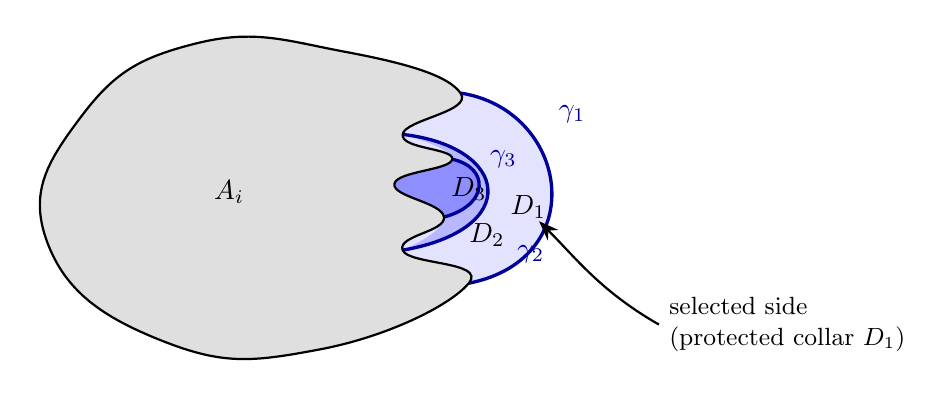
\begin{tikzpicture}[scale=1.05, line join=round]
% ---- selected domains D_1 > D_2 > D_3 (filled before the atom, which
% ---- is drawn on top and cleans up the shared boundary) ----
% D_1: region between crosscut gamma_1 and the oscillating boundary edge
\fill[blue!55, opacity=0.20]
  (0.2,1.1) .. controls (1.5,0.9) and (1.8,-0.9) .. (0.3,-1.2)
  plot [smooth, tension=0.8] coordinates
    {(0.3,-1.2) (-0.5,-0.8) (0.0,-0.4) (-0.6,0.0) (0.1,0.3) (-0.5,0.6) (0.2,1.1)};
% D_2
\fill[blue!55, opacity=0.38]
  (-0.5,0.6) .. controls (0.8,0.45) and (0.95,-0.55) .. (-0.5,-0.8)
  plot [smooth, tension=0.8] coordinates
    {(-0.5,-0.8) (0.0,-0.4) (-0.6,0.0) (0.1,0.3) (-0.5,0.6)};
% D_3
\fill[blue!55, opacity=0.60]
  (0.1,0.3) .. controls (0.55,0.2) and (0.55,-0.25) .. (0.0,-0.4)
  plot [smooth, tension=0.8] coordinates
    {(0.0,-0.4) (-0.6,0.0) (0.1,0.3)};
% ---- crosscuts ----
\draw[very thick, blue!60!black]
  (0.2,1.1) .. controls (1.5,0.9) and (1.8,-0.9) .. (0.3,-1.2);
\draw[very thick, blue!60!black]
  (-0.5,0.6) .. controls (0.8,0.45) and (0.95,-0.55) .. (-0.5,-0.8);
\draw[very thick, blue!60!black]
  (0.1,0.3) .. controls (0.55,0.2) and (0.55,-0.25) .. (0.0,-0.4);
% ---- the atom: an irregular, non-locally-connected-looking blob ----
\fill[gray!25]
  plot [smooth cycle, tension=0.8] coordinates
    {(0.2,1.1) (-1.2,1.6) (-3.0,1.7) (-4.4,0.8) (-4.8,-0.7) (-3.4,-1.9)
     (-1.5,-2.0) (0.3,-1.2) (-0.5,-0.8) (0.0,-0.4) (-0.6,0.0) (0.1,0.3)
     (-0.5,0.6)};
\draw[thick]
  plot [smooth cycle, tension=0.8] coordinates
    {(0.2,1.1) (-1.2,1.6) (-3.0,1.7) (-4.4,0.8) (-4.8,-0.7) (-3.4,-1.9)
     (-1.5,-2.0) (0.3,-1.2) (-0.5,-0.8) (0.0,-0.4) (-0.6,0.0) (0.1,0.3)
     (-0.5,0.6)};
% ---- labels ----
\node at (-2.6,-0.1) {$A_i$};
\node[blue!60!black] at (1.55,0.85) {$\gamma_1$};
\node[blue!60!black] at (1.05,-0.85) {$\gamma_2$};
\node[blue!60!black] at (0.72,0.30) {$\gamma_3$};
\node at (1.02,-0.28) {$D_1$};
\node at (0.52,-0.62) {$D_2$};
\node at (0.30,-0.06) {$D_3$};
% selected-side arrow
\draw[-{Stealth[length=2.5mm]}, thick]
  (2.6,-1.7) node[right, align=left, font=\small]
  {selected side\\ (protected collar $D_1$)}
  .. controls (1.9,-1.3) and (1.6,-0.9) .. (1.15,-0.45);
\end{tikzpicture}
\caption{A protected prime-end crosscut chain at a single atom $A_i$.  The
crosscuts $\gamma_1,\gamma_2,\gamma_3$ are pairwise disjoint arcs of
$\Chat\setminus A_i$ with endpoints on $\partial A_i$ and shrinking
diameters; the shaded regions are the nested selected sides
$D_1\supset D_2\supset D_3$, drawn with increasing opacity toward the
prime end.  The outermost selected domain $D_1$ is the protected collar of
the access: after truncation the collar tail $D_1\setminus A_i$ is
disjoint from every other collar tail, lies in $U$, and misses the
obstacle set $Z$ and the other atoms.  The boundary of the atom is drawn
deliberately oscillating: no local connectivity of $\partial A_i$ is
assumed anywhere in this section, and the access is carried entirely by
the chain, not by any landing curve.}
\label{fig:collar}
\end{figure}

\begin{definition}[Protected ribbon-routing certificate; manuscript
Definition 10.1]\label{def:certificate}
A \emph{protected ribbon-routing certificate} consists of the preceding
data---the Jordan disk $U$, the atoms $A_1,\dots,A_s$, the forbidden set
$Z$, and the truncated protected chains $\Gamma_{i,a}$---together with
pairwise disjoint \emph{free-port arcs} $\alpha_i\colon[0,1]\to U$
satisfying
\[
\alpha_i\cap A_i=\{x_i\},\qquad
\alpha_i((0,1])\cap
\Bigl(Z\cup\bigcup_{j}A_j\cup\bigcup_{j,a}D_{j,a,1}\Bigr)=\varnothing,
\]
where $x_i=\alpha_i(0)$, and an embedded finite tree $G\subset U$ joining
the outer port endpoints $\alpha_1(1),\dots,\alpha_s(1)$ while missing the
same protected and forbidden sets
$Z\cup\bigcup_jA_j\cup\bigcup_{j,a}D_{j,a,1}$.  The planar cyclic order of
half-edges at every vertex of $G$ is retained as part of the certificate
(its \emph{ribbon structure}).  Every access read by a proof must be a
protected chain $\Gamma_{i,a}$ or a declared side of this ribbon tree.
\end{definition}

Given a certificate $R$, define its \emph{carrier}
\begin{equation}\label{eq:C-HR}
H_R \;=\; G\cup\bigcup_i\alpha_i\cup\bigcup_iA_i .
\end{equation}

Four reading notes.  First, the port arc $\alpha_i$ touches its atom at
the single \emph{free port} $x_i$, a point deliberately not lying in any
protected collar: the second displayed condition includes
$a$-indexed collars of the \emph{same} atom $i$, so the port enters the
atom away from every protected access.  Second, ``joining the outer port
endpoints'' is read as part of the embeddedness of the certificate: the
tree $G$ meets each port arc $\alpha_i$ in exactly the point
$\alpha_i(1)$, so that $G\cup\bigcup_i\alpha_i$ is again an embedded
finite tree, with the port arcs attached as pendant edges.  This is the
configuration produced by the construction of
Section~\ref{sec:criterion}, where the routing tree is built in the
complement of the slit port arcs, and it is used in the proof of the
realization theorem below.  Third, the tree $G$ is a
combinatorial object with a planar enhancement: recording the cyclic order
of half-edges at each vertex fixes, up to isotopy, the two sides of every
edge, and it is these \emph{declared ribbon sides} that the realization
theorem converts into new accesses with a prescribed boundary order.
Fourth, the final sentence of the definition is a discipline on all later
arguments, not a property of the data: any subsequent proof that consults
an access of the carrier must consult either a protected chain or a
declared ribbon side, never an incidental access created by the geometry
of a particular embedding.  Figure~\ref{fig:certificate} shows a
certificate with three atoms.

\begin{figure}[htbp]
\centering
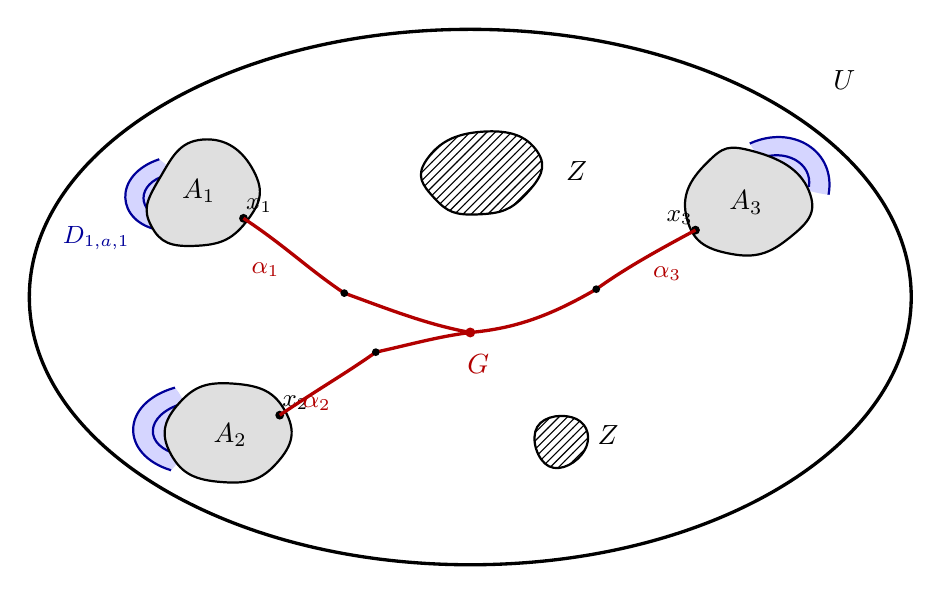
\begin{tikzpicture}[scale=1.0, line join=round]
% ---------- Jordan disk U ----------
\draw[very thick] (0,0) ellipse (5.6 and 3.4);
\node at (4.75,2.75) {$U$};
% ---------- obstacle set Z (hatched) ----------
\fill[pattern=north east lines]
  plot [smooth cycle, tension=0.9] coordinates
    {(0.1,1.05) (0.7,1.30) (0.85,1.85) (0.15,2.10) (-0.55,1.75) (-0.45,1.25)};
\draw[thick]
  plot [smooth cycle, tension=0.9] coordinates
    {(0.1,1.05) (0.7,1.30) (0.85,1.85) (0.15,2.10) (-0.55,1.75) (-0.45,1.25)};
\fill[pattern=north east lines]
  plot [smooth cycle, tension=0.9] coordinates
    {(1.0,-2.15) (1.45,-1.95) (1.35,-1.55) (0.85,-1.65)};
\draw[thick]
  plot [smooth cycle, tension=0.9] coordinates
    {(1.0,-2.15) (1.45,-1.95) (1.35,-1.55) (0.85,-1.65)};
\node at (1.35,1.6) {$Z$};
\node at (1.75,-1.75) {$Z$};
% =========== atom A_1 (upper left) ===========
% collar (faces upper-left): shaded selected side + two crosscuts
\fill[blue!55, opacity=0.30]
  (-3.95,1.75) .. controls (-4.55,1.55) and (-4.5,0.95) .. (-3.95,0.85)
  .. controls (-3.6,1.1) and (-3.6,1.5) .. cycle;
\draw[thick, blue!60!black]
  (-3.95,1.75) .. controls (-4.55,1.55) and (-4.5,0.95) .. (-3.95,0.85);
\draw[thick, blue!60!black]
  (-3.85,1.55) .. controls (-4.25,1.45) and (-4.25,1.05) .. (-3.85,1.0);
% blob
\fill[gray!25]
  plot [smooth cycle, tension=0.9] coordinates
    {(-3.4,2.0) (-2.75,1.6) (-2.85,0.95) (-3.5,0.65) (-4.05,0.9) (-3.95,1.5)};
\draw[thick]
  plot [smooth cycle, tension=0.9] coordinates
    {(-3.4,2.0) (-2.75,1.6) (-2.85,0.95) (-3.5,0.65) (-4.05,0.9) (-3.95,1.5)};
\node at (-3.45,1.35) {$A_1$};
\node[blue!60!black, font=\small] at (-4.75,0.75) {$D_{1,a,1}$};
% port
\fill (-2.88,1.0) circle (1.6pt);
\node[font=\small, above right=-2pt] at (-2.92,1.0) {$x_1$};
\draw[very thick, red!70!black]
  (-2.88,1.0) .. controls (-2.35,0.65) and (-2.05,0.35) .. (-1.6,0.05);
\node[red!70!black, font=\small] at (-2.6,0.35) {$\alpha_1$};
% =========== atom A_2 (lower left) ===========
% collar (faces left)
\fill[blue!55, opacity=0.30]
  (-3.75,-1.15) .. controls (-4.45,-1.35) and (-4.45,-2.0) .. (-3.8,-2.2)
  .. controls (-3.5,-1.9) and (-3.5,-1.45) .. cycle;
\draw[thick, blue!60!black]
  (-3.75,-1.15) .. controls (-4.45,-1.35) and (-4.45,-2.0) .. (-3.8,-2.2);
\draw[thick, blue!60!black]
  (-3.65,-1.35) .. controls (-4.15,-1.5) and (-4.15,-1.9) .. (-3.7,-2.0);
% blob
\fill[gray!25]
  plot [smooth cycle, tension=0.9] coordinates
    {(-3.0,-1.1) (-2.35,-1.45) (-2.45,-2.1) (-3.15,-2.35) (-3.8,-2.0) (-3.7,-1.35)};
\draw[thick]
  plot [smooth cycle, tension=0.9] coordinates
    {(-3.0,-1.1) (-2.35,-1.45) (-2.45,-2.1) (-3.15,-2.35) (-3.8,-2.0) (-3.7,-1.35)};
\node at (-3.05,-1.75) {$A_2$};
% port
\fill (-2.42,-1.5) circle (1.6pt);
\node[font=\small, above right=-2pt] at (-2.46,-1.5) {$x_2$};
\draw[very thick, red!70!black]
  (-2.42,-1.5) .. controls (-1.9,-1.15) and (-1.55,-0.95) .. (-1.2,-0.7);
\node[red!70!black, font=\small] at (-1.95,-1.35) {$\alpha_2$};
% =========== atom A_3 (right) ===========
% collar (faces upper right)
\fill[blue!55, opacity=0.30]
  (3.55,1.95) .. controls (4.1,2.2) and (4.65,1.85) .. (4.55,1.3)
  .. controls (4.1,1.35) and (3.75,1.6) .. cycle;
\draw[thick, blue!60!black]
  (3.55,1.95) .. controls (4.1,2.2) and (4.65,1.85) .. (4.55,1.3);
\draw[thick, blue!60!black]
  (3.65,1.75) .. controls (4.0,1.9) and (4.35,1.7) .. (4.3,1.4);
% blob
\fill[gray!25]
  plot [smooth cycle, tension=0.9] coordinates
    {(3.0,1.7) (3.6,1.85) (4.3,1.35) (4.05,0.75) (3.3,0.55) (2.75,1.0)};
\draw[thick]
  plot [smooth cycle, tension=0.9] coordinates
    {(3.0,1.7) (3.6,1.85) (4.3,1.35) (4.05,0.75) (3.3,0.55) (2.75,1.0)};
\node at (3.5,1.2) {$A_3$};
% port
\fill (2.86,0.85) circle (1.6pt);
\node[font=\small, above left=-2pt] at (2.9,0.85) {$x_3$};
\draw[very thick, red!70!black]
  (2.86,0.85) .. controls (2.3,0.55) and (1.95,0.35) .. (1.6,0.1);
\node[red!70!black, font=\small] at (2.5,0.3) {$\alpha_3$};
% =========== ribbon tree G ===========
\fill[red!70!black] (0,-0.45) circle (1.8pt);
\draw[very thick, red!70!black]
  (-1.6,0.05) .. controls (-1.05,-0.15) and (-0.55,-0.35) .. (0,-0.45);
\draw[very thick, red!70!black]
  (-1.2,-0.7) .. controls (-0.75,-0.6) and (-0.4,-0.5) .. (0,-0.45);
\draw[very thick, red!70!black]
  (1.6,0.1) .. controls (1.0,-0.25) and (0.55,-0.4) .. (0,-0.45);
\node[red!70!black] at (0.1,-0.85) {$G$};
% outer endpoints
\fill (-1.6,0.05) circle (1.4pt);
\fill (-1.2,-0.7) circle (1.4pt);
\fill (1.6,0.1) circle (1.4pt);
\end{tikzpicture}
\caption{A protected ribbon-routing certificate with three atoms inside
the Jordan disk $U$.  Each atom $A_i$ carries a protected collar (shaded,
with two nested crosscuts indicated) and a free-port arc $\alpha_i$
(heavy) landing at the single free point $x_i$, chosen away from every
protected collar.  The embedded finite tree $G$ (heavy) joins the outer
port endpoints; the interiors of the $\alpha_i$ and all of $G$ avoid the
hatched obstacle set $Z$, all atoms, and all first collars
$D_{j,a,1}$.  The planar cyclic order of the half-edges at the vertex of
$G$ is part of the certificate.  The carrier is
$H_R=G\cup\bigcup_i\alpha_i\cup\bigcup_iA_i$.}
\label{fig:certificate}
\end{figure}

\subsection*{Fullness of one-point tree attachments}
The first step of the realization is to verify that the carrier
\eqref{eq:C-HR} is a full continuum.  The union
$T=G\cup\bigcup_i\alpha_i$ is itself a finite plane tree: $G$ is a finite
tree and, by the attachment convention recorded after
Definition~\ref{def:certificate}, each $\alpha_i$ meets $G$ in exactly
the point $\alpha_i(1)$, so adjoining the arcs one at a time adds pendant
edges and creates no cycle.  By the port conditions of
Definition~\ref{def:certificate}, $T$ meets each atom $A_i$ in exactly the
point $x_i$ and otherwise misses every atom.  The relevant general fact is
the following lemma, for which we record two proofs: a direct induction on
Janiszewski's separation theorem, and a cohomological argument by
Alexander duality and Mayer--Vietoris.  The first is elementary and
self-contained; the second is the pattern that recurs, for pairwise
disjoint packets, in the packet lemmas of Section~\ref{sec:packets}.

\begin{lemma}[One-point tree attachments are full; manuscript Lemma 10.2]
\label{lem:tree-full}
If a finite plane tree meets each of finitely many pairwise disjoint full
continua in exactly one point and otherwise misses them, then their union
is a full continuum.
\end{lemma}

\begin{proof}[First proof (Janiszewski induction)]
Let $T$ be the finite plane tree and $A_1,\dots,A_s$ the pairwise disjoint
full continua, with $T\cap A_i=\{p_i\}$.  All sets are regarded as compact
subsets of the sphere $\Chat$, and \emph{nonseparating} means that the
complement in $\Chat$ is connected; for a compact subset of $\C$ this is
equivalent to fullness, since the complement in $\Chat$ is open and
connected exactly when the bounded complementary components in $\C$ are
absent.

A finite plane tree is nonseparating.  Indeed, $T$ is compact, connected,
and simply connected, and one may argue by induction on the number of
edges: a single closed arc does not separate the sphere, and if
$T=T'\cup e$ with $e$ a closed pendant edge meeting $T'$ in one endpoint,
then $T'$ and $e$ are nonseparating compacta with connected (one-point)
intersection, so Janiszewski's theorem, quoted below, makes $T$
nonseparating.

We now attach the full continua one at a time.  Put
\[
B_0=T,\qquad B_k=T\cup A_1\cup\dots\cup A_k\quad(1\le k\le s),
\]
so that $B_s$ is the union in question.  Each $B_k$ is compact, and it is
connected because $T$ is connected and each attached $A_j$ meets $T$.  We
claim every $B_k$ is nonseparating.  The case $k=0$ was just proved.
Assume $B_{k-1}$ is nonseparating and consider $B_k=B_{k-1}\cup A_k$.
The intersection is
\[
B_{k-1}\cap A_k
=(T\cap A_k)\cup\bigcup_{j<k}(A_j\cap A_k)
=\{p_k\},
\]
a singleton, hence connected: the atoms are pairwise disjoint and $T$
meets $A_k$ only at $p_k$.  Both $B_{k-1}$ and $A_k$ are compact and
nonseparating.  Janiszewski's separation theorem
\cite{New51,Why42} states that if two closed subsets of the sphere have
connected intersection and neither separates a given pair of points, then
their union does not separate that pair.  Applying this to every pair of
points of $\Chat\setminus B_k$ shows that $B_k$ separates no pair of
points of its complement, that is, $B_k$ is nonseparating.  By induction,
$B_s$ is a compact connected set with connected complement in $\Chat$,
hence a full continuum.
\end{proof}

\begin{proof}[Second proof (Alexander duality and Mayer--Vietoris)]
Work again in $\Chat=S^2$ and retain the notation $B_k$ of the first
proof.  For a compact set $X\subset S^2$, Alexander duality in its
\v{C}ech form \cite{Hat02} gives an isomorphism
\[
\widetilde H_0\bigl(S^2\setminus X;\Z\bigr)\;\cong\;\check H^1(X;\Z),
\]
so $X$ is nonseparating precisely when its first reduced \v{C}ech
cohomology vanishes.  (\v{C}ech cohomology is essential here: the atoms
are arbitrary continua, in general not locally connected, and no
CW-approximation of them is available; \v{C}ech theory has the required
continuity under inverse limits of neighborhoods and satisfies the
Mayer--Vietoris sequence for compact pairs in a normal ambient space.)

The tree $T$ is contractible, so $\check H^1(T;\Z)=0$; and
$\check H^1(A_i;\Z)=0$ for every $i$ because each $A_i$ is full, by the
same duality read in the other direction.  Now induct on $k$.  Suppose
$\check H^1(B_{k-1};\Z)=0$ and write $B_k=B_{k-1}\cup A_k$ with
$B_{k-1}\cap A_k=\{p_k\}$.  The Mayer--Vietoris sequence in reduced
\v{C}ech cohomology for the compact pair $(B_{k-1},A_k)$ reads
\[
\widetilde{\check H}^0(\{p_k\};\Z)
\longrightarrow
\check H^1(B_k;\Z)
\longrightarrow
\check H^1(B_{k-1};\Z)\oplus\check H^1(A_k;\Z).
\]
The left group vanishes because the one-point intersection is connected,
and the right group vanishes by the inductive hypothesis and fullness of
$A_k$.  Exactness forces $\check H^1(B_k;\Z)=0$.  By induction
$\check H^1(B_s;\Z)=0$, and Alexander duality converts this back into
connectedness of $S^2\setminus B_s$.  Since $B_s$ is compact and
connected, it is a full continuum.
\end{proof}

The two proofs establish literally the same induction step, and the
translation between them is the dictionary used throughout this paper:
``nonseparating'' equals ``vanishing first \v{C}ech cohomology,''
``connected intersection'' equals ``vanishing zeroth reduced cohomology of
the overlap.''  The cohomological form is the one that survives when the
finitely many one-point overlaps are replaced by the pairwise
\emph{disjoint} packets of Section~\ref{sec:packets}, where the nerve
argument of Lemma~\ref{lem:packets} takes over.

\subsection*{Survival of protected chains}
The second step is the heart of the realization: enlarging an atom to a
full continuum that stays out of a protected collar does not damage the
protected access.  The chain survives verbatim---the same crosscuts, the
same selected sides---as a prime-end chain of the complement of the
enlarged continuum, and finitely many protected accesses with disjoint
collars stay distinct and keep their cyclic order.

\begin{lemma}[Protected crosscut survival and order; manuscript
Lemma 10.3]\label{lem:crosscut-survival}
Let $H\supset A_i$ be a full continuum and let $(\gamma_n,D_n)_{n\ge1}$ be
one of the protected chains above.  If
\[
(H\setminus A_i)\cap(D_1\setminus A_i)=\varnothing,
\]
then a tail of the same crosscuts is a prime-end chain in
$\Chat\setminus H$.  Its endpoints remain boundary points and its selected
sides contain the old $D_n$.  A finite family of such chains with pairwise
disjoint terminal selected domains induces distinct prime ends of
$\Chat\setminus H$ with unchanged cyclic order.
\end{lemma}

\begin{proof}
Since $H$ is a full continuum, $\Chat\setminus H$ is a simply connected
domain and has its own prime-end theory.  We verify that the tail
$(\gamma_n)_{n\ge2}$, with the same selected sides, is a null chain for
it.

\emph{The selected domains avoid $H$ entirely.}
For every $n$ the selected domain $D_n$ lies in $\Chat\setminus A_i$, so
$D_n\setminus A_i=D_n$, and it is contained in $D_1$ by nestedness.
Hence
\[
H\cap D_n
=(A_i\cap D_n)\cup\bigl((H\setminus A_i)\cap D_n\bigr)
\subset\varnothing\cup\bigl((H\setminus A_i)\cap(D_1\setminus A_i)\bigr)
=\varnothing,
\]
so $D_n\subset\Chat\setminus H$ for every $n$.

\emph{Each deep crosscut remains a crosscut.}
Fix $n\ge2$.  The open arc $\gamma_n$ lies in $D_{n-1}\subset D_1$:
indeed $\gamma_n$ lies in the closure of $D_n\subset D_{n-1}$ and in
$\Chat\setminus A_i$, and the part of $\partial D_{n-1}$ inside
$\Chat\setminus A_i$ is $\gamma_{n-1}$, which $\gamma_n$ misses.  So by
the preceding paragraph the arc $\gamma_n$ misses $H$; its two distinct
endpoints lie on $\partial A_i$, hence in $A_i\subset H$.  Every
neighborhood of either endpoint meets the crosscut interior, which
consists of points of $\Chat\setminus H$, so both endpoints remain
boundary points of the enlarged complement $\Chat\setminus H$, and they
are still distinct.  Thus $\gamma_n$ is again an open Jordan arc in
$\Chat\setminus H$ whose closure is an arc with two distinct endpoints on
$\partial(\Chat\setminus H)$, that is, a crosscut of $\Chat\setminus H$.

\emph{The selected sides are unchanged.}
For $n\ge2$ let $D_n'$ denote the component of
$(\Chat\setminus H)\setminus\gamma_n$ containing $D_n$; this is
well defined because $D_n$ is connected and disjoint from
$H\cup\gamma_n$.  We claim $D_n'=D_n$, so that the containment
$D_n'\supset D_n$ asserted in the statement holds with equality.  The
set $D_n$ is open, and it is relatively closed in
$(\Chat\setminus H)\setminus\gamma_n$: as a component of the open set
$(\Chat\setminus A_i)\setminus\gamma_n$ it satisfies
\[
\partial D_n
\subset\partial A_i\cup\overline{\gamma_n}
\subset A_i\cup\gamma_n
\subset H\cup\gamma_n,
\]
since the closure of the open arc $\gamma_n$ adds only its two
endpoints, which lie in $A_i$; hence no boundary point of $D_n$ belongs
to $(\Chat\setminus H)\setminus\gamma_n$, and every point of that set
lying in $\overline{D_n}$ already lies in $D_n$.  A nonempty connected
subset of an open set that is both open and relatively closed is a
component of it, so $D_n'=D_n$.  Nestedness of the new sides is now
inherited from the original chain:
$D_{n+1}'=D_{n+1}\subset D_n=D_n'$ for every $n\ge2$, and
$\gamma_{n+1}\subset D_n=D_n'$ lies in the selected side of $\gamma_n$,
as a null chain requires.

\emph{The diameters still tend to zero.}
The crosscuts are unchanged as point sets, so their spherical diameters
are the same numbers as before and still tend to zero.  Consequently
$(\gamma_n,D_n')_{n\ge2}$ is a prime-end chain of $\Chat\setminus H$,
which proves the first two assertions.

\emph{Distinctness.}
Now consider a finite family of protected chains satisfying the
hypothesis, with pairwise disjoint terminal selected domains.  Recall
that two null chains of the same domain define the same prime end if and
only if they eventually divide one another: every selected domain of
either chain contains all sufficiently deep selected domains of the
other.  Suppose two chains of the family, with terminal domains
$D_1^{(1)}$ and $D_1^{(2)}$, induced the same prime end of
$\Chat\setminus H$.  Then some deep selected domain of the first
chain---by the preceding step, the same set $D_m^{(1)}$ as before the
enlargement---would be contained in a selected domain of the second
chain, hence in $D_1^{(2)}$; but that deep domain is nonempty and
contained in $D_1^{(1)}$, contradicting
$D_1^{(1)}\cap D_1^{(2)}=\varnothing$.  Disjoint terminal domains
therefore prevent mutual division, and the induced prime ends are
pairwise distinct.  In particular the survival map, from protected
chains to prime ends of $\Chat\setminus H$, is injective on such a
family.

\emph{Cyclic order.}
The prime ends of the simply connected domain $\Chat\setminus H$ carry a
natural cyclic order, the one transported from the unit circle by a
Riemann map \cite{Pom92}.  For a finite family of prime ends represented
by pairwise disjoint crosscuts whose selected sides are also pairwise
disjoint, this order can be read off inside the domain, as follows.
Choose one deep crosscut from each chain, deep enough that the chosen
crosscuts lie in the pairwise disjoint terminal collars; then the chosen
crosscuts are pairwise disjoint and their selected sides are pairwise
disjoint.  Fix three chains of the family, with chosen crosscuts
$c_1,c_2,c_3$ and selected sides $S_1,S_2,S_3$.  Call an embedded triod
$Y$---three arcs with a common branch point, disjoint except at that
point---\emph{computing} if $Y$ lies in the domain and meets the
configuration $\bigcup_{k=1}^{3}(c_k\cup S_k)$ in exactly its three leg
tips, one tip on each $c_k$.  Transporting by a Riemann map turns the
configuration into three pairwise disjoint crosscuts of the unit disk
cutting off pairwise disjoint caps, and a computing triod into an
embedded triod tipping on the three crosscuts and otherwise avoiding
crosscuts and caps.  In the disk, computing triods exist, and the cyclic
order of the three legs at the branch point of any computing triod
agrees with the cyclic order of the three caps on the circle, that is,
with the cyclic order of the three prime ends: the complement of the
three open caps in the closed disk is a closed Jordan region whose
boundary traverses the three crosscuts in the cyclic order of the caps,
and an embedded triod in a Jordan region whose legs end on three
disjoint boundary arcs realizes at its branch point exactly the cyclic
order of those arcs.  Hence, back in the original domain, computing
triods exist for every triple of chains, and each one realizes the
cyclic orientation of its prime-end triple at its branch point.

Now compare the two domains.  By the preceding steps, the chosen
crosscuts and their selected sides are \emph{literally the same sets}
for $\Chat\setminus A_i$ and for $\Chat\setminus H$.  Fix a triple of
chains and choose a computing triod $Y$ in the smaller domain
$\Chat\setminus H$.  Since $\Chat\setminus H\subset\Chat\setminus A_i$
and the configuration is unchanged, $Y$ is simultaneously a computing
triod in $\Chat\setminus A_i$.  Reading the branch point of this one
triod in both domains shows that the prime-end triple has the same
cyclic orientation in $\Chat\setminus H$ as in $\Chat\setminus A_i$.
Every ordered triple therefore retains its orientation, and the cyclic
order of the whole family is unchanged.
\end{proof}

\subsection*{The realization theorem}
Assembling the two lemmas yields the main result of this section.

\begin{theorem}[Protected regulated connector realization; manuscript
Theorem 10.4]\label{thm:realization}
Every protected ribbon-routing certificate $R$ has an actual carrier
$H_R$, given by \eqref{eq:C-HR}, with the following properties:
\begin{enumerate}
\item $H_R\Subset U$ is compact, connected, and full;
\item it contains every $A_i$, misses $Z$, and has singleton attachment
trace $\{x_i\}$ at each atom;
\item every protected crosscut chain remains a prime-end chain in
$\Chat\setminus H_R$;
\item the survival map is injective and preserves cyclic order;
\item the connector-created sides have the boundary order of the retained
ribbon tree; and
\item no local connectivity of any $A_i$ is required.
\end{enumerate}
\end{theorem}

\begin{proof}
\emph{Clause} (1).  As observed before Lemma~\ref{lem:tree-full}, the set
$T=G\cup\bigcup_i\alpha_i$ is a finite plane tree meeting each atom $A_i$
in exactly the point $x_i$ and otherwise missing every atom.
Lemma~\ref{lem:tree-full} applies to $T$ and $A_1,\dots,A_s$ and shows
that $H_R=T\cup\bigcup_iA_i$ is a full continuum.  Each constituent is
compactly contained in $U$, and there are finitely many, so
$H_R\Subset U$.

\emph{Clause} (2).  Containment of the atoms is part of
\eqref{eq:C-HR}.  The certificate conditions of
Definition~\ref{def:certificate} state that the arcs
$\alpha_i((0,1])$ and the tree $G$ miss $Z$, and $Z$ misses every atom by
hypothesis, so $H_R\cap Z=\varnothing$.  The attachment trace at $A_i$ is
the intersection of $A_i$ with the connector: $T\cap A_i=\{x_i\}$ because
$\alpha_i\cap A_i=\{x_i\}$, the other port arcs and $G$ miss $A_i$, and
the atoms are pairwise disjoint.

\emph{Clause} (3).  Fix a protected chain $\Gamma_{i,a}$.  We verify the
hypothesis of Lemma~\ref{lem:crosscut-survival} for $H=H_R$ and the atom
$A_i$.  The difference $H_R\setminus A_i$ is contained in
\[
G\cup\bigcup_j\alpha_j((0,1])\cup\bigcup_{j\ne i}A_j .
\]
The tree $G$ and every half-open port arc $\alpha_j((0,1])$ miss
\emph{all} first collars $D_{j',a',1}$, in particular $D_{i,a,1}$, by
Definition~\ref{def:certificate}; and each atom $A_j$ with $j\ne i$
misses the collar tail $D_{i,a,1}\setminus A_i$ by the truncation
normalization.  Hence
$(H_R\setminus A_i)\cap(D_{i,a,1}\setminus A_i)=\varnothing$: the
connector misses the terminal collar tail, and therefore misses every
later closed collar tail $D_{i,a,n}\subset D_{i,a,1}$ as well.
Lemma~\ref{lem:crosscut-survival} now shows that a tail of
$\Gamma_{i,a}$ is a prime-end chain in $\Chat\setminus H_R$.

\emph{Clause} (4).  The truncation normalization makes the terminal
selected domains of distinct protected chains pairwise disjoint.  For
each atom $A_i$, the final part of Lemma~\ref{lem:crosscut-survival}
with $H=H_R$ gives distinctness and preservation of cyclic order for the
subfamily of chains protecting $A_i$.  The distinctness argument of the
lemma uses only disjointness of the terminal selected domains and
survival of both chains in $\Chat\setminus H_R$, so it applies verbatim
to a pair of chains protecting different atoms as well.  The survival
map is therefore injective on the full family over all $(i,a)$, and it
preserves the cyclic order of every protected family with a common
source domain.

\emph{Clause} (5).  Let $N$ be a small regular neighborhood of the finite
connector tree $T$ in the plane, chosen so thin that $N$ misses $Z$ and
meets each atom only near its port point.  A regular neighborhood of a finite plane tree is a closed
disk, and its boundary circle traverses every edge of $T$ on two sides:
following $\partial N$, one passes along each edge once in each
direction, and at a vertex of valence $d$ the boundary visits the $d$
half-edges in exactly their planar cyclic order.  The resulting cyclic
\emph{boundary word}, in which every edge appears twice with opposite
orientations, is precisely the boundary word of the ribbon structure
retained in the certificate.  The accesses to $H_R$ created by the
connector---the two sides of every edge of $G$ and of every port
arc---are read along this boundary circle, so their boundary order is the
boundary order of the retained ribbon tree, as claimed.

\emph{Clause} (6).  The argument uses crosscut chains only: atoms enter
through their prime-end chains and through the single point $x_i$, never
through a boundary parametrization.  No Euclidean boundary extension of
any $A_i$---in particular no continuity of a Riemann map up to the
boundary, equivalently no local connectivity of any atom---is assumed at
any step.
\end{proof}

\begin{remark}\label{rem:C-no-lc}
Clause (6) is the point of the whole construction and deserves emphasis.
Realization arguments for connectors frequently assume that accesses
land, that is, that radial limits of Riemann maps exist at the relevant
boundary points; by Carath\'eodory's theorem this amounts to local
connectivity of the atom boundaries.  The certificate formalism removes
that hypothesis: an access is a chain of crosscuts with declared sides,
an object available for an arbitrary full continuum, and
Lemma~\ref{lem:crosscut-survival} shows it is preserved verbatim under
any enlargement respecting the collar.  This is what allows the framework
to be applied, in Section~\ref{sec:decoration}, to atoms that are not
known---and are not claimed---to be locally connected.
\end{remark}

\subsection*{Univalent naturality}
The certificate data and the carrier construction are natural under
univalent change of the Jordan localization.

\begin{proposition}[Univalent naturality; manuscript Proposition 10.5]
\label{prop:naturality}
If $\phi\colon U\to V$ is an orientation-preserving conformal
homeomorphism of Jordan disks and every certificate entry is transported
by $\phi$, then
\begin{equation}\label{eq:C-naturality}
H_{\phi_*R}=\phi(H_R).
\end{equation}
The protected survival map and the ribbon boundary order commute with the
prime-end map induced by $\phi$.
\end{proposition}

\begin{proof}
Since $U$ and $V$ are Jordan disks, Carath\'eodory's extension theorem
\cite{Pom92} extends $\phi$ to a homeomorphism
$\overline U\to\overline V$ of the closed disks.  By the Schoenflies
theorem the restricted boundary homeomorphism
$\partial U\to\partial V$ extends to a homeomorphism of the complementary
closed disks $\Chat\setminus U\to\Chat\setminus V$, and gluing the two
extensions along the boundary curves produces an orientation-preserving
homeomorphism $\Phi\colon\Chat\to\Chat$ with $\Phi|_U=\phi$.

A sphere homeomorphism preserves every notion entering
Definition~\ref{def:certificate} and Theorem~\ref{thm:realization}: it
carries compact connected sets to compact connected sets and complements
to complements, hence preserves fullness; it carries open Jordan arcs
with endpoints on a boundary to the same, hence crosscuts to crosscuts;
it maps the two complementary sides of a crosscut to the two sides of the
image crosscut, hence selected sides to selected sides; it carries null
chains to null chains (spherical diameters are not literally preserved,
but by uniform continuity of $\Phi$ the image crosscuts of a null chain
again have diameters tending to zero); it preserves intersections, so the
port conditions $\alpha_i\cap A_i=\{x_i\}$ and all disjointness
requirements transport; and, being orientation preserving, it preserves
the planar cyclic order of half-edges at the tree vertices and the cyclic
order of prime ends.  Consequently the transported data---the disk $V$,
the atoms $\phi(A_i)$, the obstacle $\phi(Z)$, the chains
$\Phi(\Gamma_{i,a})$, the ports $\phi\circ\alpha_i$, and the tree
$\phi(G)$ with its transported ribbon structure---form a protected
ribbon-routing certificate in $V$.  The defining union \eqref{eq:C-HR}
then transports term by term:
\[
H_{\phi_*R}
=\phi(G)\cup\bigcup_i\phi(\alpha_i)\cup\bigcup_i\phi(A_i)
=\phi\Bigl(G\cup\bigcup_i\alpha_i\cup\bigcup_iA_i\Bigr)
=\phi(H_R),
\]
which is \eqref{eq:C-naturality}.  Because $\Phi$ maps
$\Chat\setminus H_R$ onto $\Chat\setminus H_{\phi_*R}$ carrying null
chains to null chains and preserving their division relation, it induces
a bijection of prime ends under which the survival map of
Lemma~\ref{lem:crosscut-survival} for $H_R$ corresponds to the survival
map for $H_{\phi_*R}$, and the ribbon boundary words of
Theorem~\ref{thm:realization}(5) correspond letter by letter.
\end{proof}

Consequently one actual anchor certificate transports through the
complete degree-one corridor of the source manuscript \cite{MWman}.  We
record the manuscript's caveat: this transport does \emph{not} prove
equality of the transported carrier with any carrier copy supplied by the
$\psi$-ql immersion.  Naturality moves a certificate and its realization
along a univalent map; it does not identify the result with an
independently constructed carrier, and no such identification is claimed
anywhere in this paper.

With realization settled, the burden shifts to existence: when do the
port arcs and the routing tree demanded by
Definition~\ref{def:certificate} exist at all?
Section~\ref{sec:criterion} answers this question exactly, in terms of a
single component of the frozen free domain $\Omfree$ admitting
simultaneous singleton ports to every required atom.
% ---- end C:certificates ----

% ---- begin D:criterion ----
% Cluster D: the repaired slit lemma and the exact free-component criterion
% Body-only LaTeX; uses only preamble macros and fixed cross-cluster labels.

\section{The exact free-component criterion}\label{sec:criterion}

Theorem~\ref{thm:realization} converts a protected ribbon-routing certificate into an
actual carrier, but it leaves open the question of when such a certificate exists: the
embedded finite tree of Definition~\ref{def:certificate} looks like an arbitrary choice,
and one might fear that its existence depends on delicate features of the atoms or of the
forbidden data. The present section removes the arbitrary tree choice. We prove that the
existence of a protected ribbon-routing certificate is governed by a single, exact,
purely planar condition: one component of a frozen free domain must reach every required
atom by a singleton port. The section carries the one intentional mathematical divergence
of this paper from the source manuscript \cite{MWman}: the slit lemma below is stated and
proved in a repaired form, and the proof of the criterion is rewritten to match. The
divergence is recorded precisely in Remark~\ref{rem:repair}.

\subsection{The frozen free domain}\label{subsec:D-frozen}

Freeze the complete finite future inventory before choosing a connector. Concretely, let
$U$ be the Jordan localization and let $Q\subset U$ be the union of
all root-shadow atoms $A_1,\dots,A_s$, the closed terminal protected collars of every
protected prime-end chain in the inventory, the separated obstacles, the critical-value
exclusion, and the localization-forbidden set. As a standing convention, following the
compact-containment hypotheses of the certificate setup, we assume each constituent of
$Q$ is closed in $U$ and that the atoms, collars, and obstacles are compactly contained
in $U$; this guarantees that the free domain defined next is open. Put
\begin{equation}\label{eq:D-free-domain}
\Omfree \;=\; U\setminus Q
\end{equation}
(equation~(9.4) of the manuscript \cite{MWman}). The set $\Omfree$ is open, and its
connected components are plane domains, the \emph{free components} of the frozen data.

A component $\Omega_0$ of $\Omfree$ \emph{has simultaneous singleton ports} to the
required atoms if there are pairwise disjoint Jordan arcs
$\alpha_1,\dots,\alpha_s\colon[0,1]\to U$ such that, for every $i$, the arc $\alpha_i$
meets $A_i$ exactly in the single point $x_i=\alpha_i(0)$ and satisfies
$\alpha_i\bigl((0,1]\bigr)\subset\Omega_0$. The landing point $x_i$ is called a
\emph{free point} of $A_i$ because it is reached from the free domain; no further
property of $x_i$ is assumed at this stage. (Compare the unprotected exposure loci of
Lemma~\ref{lem:port-localization}, where an additional protected-impression exclusion is
imposed; the interaction between the two notions is illustrated in
Example~\ref{ex:no-common-component} below.)

The adjective \emph{frozen} is load-bearing, and we emphasize it once. The set $Q$ lists
the complete finite future inventory: every atom that will ever have to be joined, the
closed terminal collar of every protected chain that any future step of a proof will
read, every obstacle that must remain separated, the full critical-value exclusion, and
the localization-forbidden set. This list is fixed \emph{before} any connector is chosen.
Nothing may be added to $Q$ afterwards, and nothing may be removed from it; all later
monotone operations act on proposed connectors, never on the inventory. This discipline
is exactly what gives the criterion of Theorem~\ref{thm:free-component} its
if-and-only-if form, and what makes its failure clause persistent: a separation already
visible in the frozen data can never be talked away by enlarging a connector. The
horizon-first closure results of the manuscript \cite{MWman} address how such an
inventory stabilizes; here the inventory is simply given, finite, and immutable.

\subsection{The repaired slit lemma}\label{subsec:D-slits}

The sufficiency direction of the criterion rests on the fact that finitely many pairwise
disjoint one-ended slits do not disconnect a plane domain. This is Lemma~10.7 of the
manuscript. Its printed statement contains a formal inconsistency (a map into an open
domain cannot take a boundary value) together with an endpoint mismatch with its
intended application; both defects are repaired in the statement below, and
Remark~\ref{rem:repair} records the divergence. The mathematical core of the
manuscript's argument --- the transverse-rectangle detour around the free endpoint ---
is retained in full.

\begin{lemma}[One-ended slits do not disconnect a plane domain; manuscript Lemma 10.7,
repaired]\label{lem:slits}
Let $\Omega\subset\C$ be a domain and let
$\delta_1,\dots,\delta_s\colon[0,1]\to\overline{\Omega}$ be Jordan arcs with pairwise
disjoint images such that $\delta_i(0)\in\partial\Omega$ and
$\delta_i\bigl((0,1]\bigr)\subset\Omega$ for every $i$. Then
\[
\Omega\setminus\bigcup_{i=1}^{s}\delta_i\bigl((0,1)\bigr)
\]
is path connected; in particular every free endpoint $\delta_i(1)$ lies in this set and
can be joined inside it to every other point of it.
\end{lemma}

\begin{proof}
Call $\delta_i$ the \emph{$i$-th slit}, write
$\sigma_i:=\delta_i\bigl((0,1]\bigr)$ for its \emph{half-open} part and
$\sigma_i^{\circ}:=\delta_i\bigl((0,1)\bigr)$ for its \emph{open} part, and call
$\delta_i(1)$ its \emph{tip}. The set to be proved path connected is
$\Omega\setminus\bigcup_i\sigma_i^{\circ}$, which contains all $s$ tips. If $s=0$ there
is nothing to prove, so assume $s\ge1$; then $\partial\Omega\neq\varnothing$.

\emph{Step 0: two preliminary observations.}
First, each half-open part $\sigma_i$ is relatively closed in $\Omega$. Indeed, the
closure of $\sigma_i$ in $\C$ is the compact arc $\delta_i([0,1])$, so the only point of
$\overline{\sigma_i}\setminus\sigma_i$ is $\delta_i(0)\in\partial\Omega$, which does not
lie in $\Omega$. Consequently $\Omega\setminus\sigma_i$ is open. By contrast, the open
part $\sigma_i^{\circ}$ is \emph{not} relatively closed in $\Omega$: its closure inside
$\Omega$ also contains the tip $\delta_i(1)\in\Omega$. This distinction is precisely the
point at which the manuscript's induction required repair; the proof below removes the
half-open parts first and reattaches the tips afterwards.

Second, every Jordan arc in the plane is tame: it can be extended to a Jordan curve,
and the Schoenflies theorem then supplies a homeomorphism of $\C$ carrying the curve to
a round circle and the arc to a circular subarc, hence, after one more homeomorphism,
onto the straight segment $[0,1]\times\{0\}$; see, e.g.,
\cite{New51,Why42}. Since path connectivity is a topological invariant and a
homeomorphism of $\C$ carries domains to domains and boundaries to boundaries, we may
straighten any \emph{single} slit whenever convenient. (Straightening one slit will in
general bend the others; each step below straightens only the slit it is processing.)

\emph{Step 1: removing a single half-open slit leaves a domain.}
Let $\Omega$ be a domain and let $\delta$ be a single arc as in the statement, with
half-open part $\sigma=\delta\bigl((0,1]\bigr)$. We claim that
$\Omega':=\Omega\setminus\sigma$ is again a domain. Openness was proved in Step~0, so
only path connectivity is at issue. By tameness we may assume, after a homeomorphism of
$\C$, that
\[
\delta(t)=(t,0)\quad(0\le t\le1),
\]
so that $\Omega$ is a domain containing $S:=(0,1]\times\{0\}$, with
$(0,0)\in\partial\Omega$, and we must join two arbitrary points
$x,y\in\Omega\setminus S$ by a path in $\Omega\setminus S$.

\emph{(a) A polygonal start missing an initial tail.}
Since a plane domain is polygonally connected \cite{New51}, choose a polygonal path
$P\subset\Omega$ from $x$ to $y$. The path $P$ is compact and does not contain the
boundary point $(0,0)$, so
\[
r:=\dist\bigl((0,0),P\bigr)>0 .
\]
Fix $\varepsilon:=\tfrac12\min(r,1)$. Every point of the initial tail
$[0,\varepsilon]\times\{0\}$ lies within distance $\varepsilon<r$ of the origin, so $P$
misses $[0,\varepsilon]\times\{0\}$. This is the only part of the closed slit that a
compact subset of $\Omega$ cannot in general avoid by compactness alone: the closed slit
image leaves every compact subset of $\Omega$ only along points accumulating at
$\delta(0)=(0,0)\in\partial\Omega$, and near that end the continuity of $\delta$ at $0$
confines the slit to a small disk around the origin. The remaining part
$\delta([\varepsilon,1])=[\varepsilon,1]\times\{0\}$ is a compact subset of $\Omega$ and
will be handled by explicit detours.

\emph{(b) A thin rectangle around the compact subarc.}
The segment $[\varepsilon,1]\times\{0\}$ lies in $\Omega$, and $(1,0)\in\Omega$ is an
interior point of $\Omega$; hence there is $\eta\in(0,\tfrac12)$ with
$[1,1+\eta]\times\{0\}\subset\Omega$. The segment
$L:=[\varepsilon/2,\,1+\eta]\times\{0\}$ is then a compact subset of $\Omega$, so
$\dist(L,\C\setminus\Omega)>0$, and we may choose
$h\in\bigl(0,\min(\varepsilon/2,\dist(L,\C\setminus\Omega)/2)\bigr)$ and set
\[
R:=[\varepsilon/2,\,1+\eta]\times[-h,h]\subset\Omega .
\]
The rectangle $R$ meets the closed slit $[0,1]\times\{0\}$ exactly in the core
$c:=[\varepsilon/2,\,1]\times\{0\}$: the slit enters $R$ through the midpoint of its
left short side and terminates at the tip $(1,0)$, an interior point of $R$. In
particular $R\cap S=[\varepsilon/2,1]\times\{0\}=c$.

We record the key connectivity property of the slit rectangle: \emph{$R\setminus c$ is
path connected.} Indeed, let $V:=\{1+\eta/2\}\times[-h,h]$, a vertical segment in $R$
missing $c$. A point of $R\setminus c$ with ordinate $y\neq0$ travels horizontally to
the point of $V$ with the same ordinate; the horizontal path misses the axis
$\mathbb{R}\times\{0\}$ entirely, hence misses $c$. A point of $R\setminus c$ with
ordinate $0$ has abscissa in $(1,1+\eta]$ and travels along the axis to $(1+\eta/2,0)$;
this path keeps abscissa $>1$, hence misses $c$. Since $V$ is connected, the claim
follows. Geometrically: the two long sides of $R$ are joined to each other inside
$R\setminus c$ \emph{around the tip}, by crossing the axis at abscissae beyond $1$.

\emph{(c) Transverse perturbation and detour repair.}
Perturb the interior vertices of $P$, keeping the endpoints $x,y$ fixed, so that no
interior vertex lies on the axis $\mathbb{R}\times\{0\}$ and no edge of $P$ is collinear
with the axis; if an endpoint happens to lie on the axis (necessarily off $S$), perturb
its adjacent vertex so that the incident edge is not horizontal. Since $P$ is compact
with $\dist(P,\C\setminus\Omega)>0$ and $\dist\bigl(P,[0,\varepsilon]\times\{0\}\bigr)
\ge r-\varepsilon>0$, a sufficiently small such perturbation keeps $P$ inside $\Omega$
and away from the initial tail. After the perturbation, every edge of $P$ meets the axis
in at most one point, and every meeting point interior to an edge is a transverse
crossing. Hence $P$ meets $S$ in finitely many points, all of the form $P(t_j)$ with
parameters $0<t_1<\dots<t_m<1$ interior to edges, and all lying in
$( \varepsilon,1]\times\{0\}\subset\Int R$. (If $m=0$, the path $P$ already joins $x$ to
$y$ in $\Omega\setminus S$ and Step~1 is complete.)

By transversality, for each $j$ there is $\rho_j>0$ such that the parameter interval
$[t_j-\rho_j,\,t_j+\rho_j]$ has image in $\Int R$, meets the axis only at $t_j$, and the
two punctured halves of the image lie strictly on opposite sides of the axis; shrink the
$\rho_j$ so that these intervals are pairwise disjoint and avoid $0$ and $1$. Put
$p_j^{-}:=P(t_j-\rho_j)$ and $p_j^{+}:=P(t_j+\rho_j)$; both lie in $R\setminus c$.
Now modify $P$ as follows: on each interval $[t_j-\rho_j,\,t_j+\rho_j]$, replace the
sub-path of $P$ by a path from $p_j^{-}$ to $p_j^{+}$ inside $R\setminus c$, which
exists by (b); keep $P$ unchanged elsewhere. Each detour lies in $R\subset\Omega$ and
misses $S$, because $S\cap R=c$ and the detour misses $c$, while $S\setminus R$ is
disjoint from $R$. The unchanged pieces of $P$ carry parameters outside the intervals
$(t_j-\rho_j,\,t_j+\rho_j)$ and therefore avoid $S$, since the crossings $t_j$ were the
only parameters at which $P$ met $S$. The concatenation is a path from $x$ to $y$ in
$\Omega\setminus S$.

Observe that each detour crosses the axis only at abscissae strictly beyond $1$: it
travels \emph{around} the tip, through points arbitrarily close to $\delta(1)$ but never
through any point of the closed slit; the tip itself, which here has been removed
together with the rest of $\sigma$, is not needed as a way-station. This completes
Step~1: $\Omega'=\Omega\setminus\sigma$ is a domain.

\emph{Step 2: removing all half-open slits leaves a domain.}
Set $\Omega_{(0)}:=\Omega$ and, inductively,
$\Omega_{(j)}:=\Omega_{(j-1)}\setminus\sigma_j$ for $1\le j\le s$. We claim that each
$\Omega_{(j)}$ is a domain and that $\delta_j$ is a one-ended slit of $\Omega_{(j-1)}$
in the sense of the statement. Indeed, suppose $\Omega_{(j-1)}$ is a domain. Because the
slit images are pairwise disjoint, $\sigma_j$ is disjoint from
$\sigma_1,\dots,\sigma_{j-1}$, so $\sigma_j\subset\Omega_{(j-1)}$. The point
$\delta_j(0)$ lies outside $\Omega\supset\Omega_{(j-1)}$, and it is the limit of the
points $\delta_j(t)\in\Omega_{(j-1)}$ as $t\downarrow0$; hence
$\delta_j(0)\in\partial\Omega_{(j-1)}$ and
$\delta_j\colon[0,1]\to\overline{\Omega_{(j-1)}}$. Step~1, applied to the domain
$\Omega_{(j-1)}$ and the single slit $\delta_j$, now shows that $\Omega_{(j)}$ is a
domain. After $s$ steps we conclude: the set
\[
\Omega_{(s)}\;=\;\Omega\setminus\bigcup_{i=1}^{s}\sigma_i
\;=\;\Omega\setminus\bigcup_{i=1}^{s}\delta_i\bigl((0,1]\bigr)
\]
is open and path connected.

\emph{Step 3: reattaching the tips.}
The set whose path connectivity is asserted differs from $\Omega_{(s)}$ exactly by the
$s$ tips:
\[
\Omega\setminus\bigcup_{i=1}^{s}\sigma_i^{\circ}
\;=\;\Omega_{(s)}\,\cup\,\{\delta_1(1),\dots,\delta_s(1)\},
\]
and the tips are pairwise distinct points not in $\Omega_{(s)}$. Since $\Omega_{(s)}$ is
path connected, it suffices to join each tip to some point of $\Omega_{(s)}$ by a path
which, apart from the tip itself, lies in $\Omega_{(s)}$.

Fix $i$ and straighten the $i$-th slit: let $\Phi$ be a homeomorphism of $\C$ with
$\Phi\bigl(\delta_i([0,1])\bigr)=[0,1]\times\{0\}$ and $\Phi(\delta_i(t))=(t,0)$. The
union $K:=\bigcup_{k\neq i}\delta_k([0,1])$ of the other closed slit images is compact
and disjoint from $\delta_i([0,1])$, so $\Phi(K)$ is compact and disjoint from
$[0,1]\times\{0\}$. The model tip $(1,0)$ lies in the open set $\Phi(\Omega)$ and
outside the closed set $\Phi(K)$, so
\[
\mu:=\dist\Bigl((1,0),\,\Phi(K)\cup\bigl(\C\setminus\Phi(\Omega)\bigr)\Bigr)>0 .
\]
Choose $a\in\bigl(0,\min(\mu/2,\tfrac12)\bigr)$ and consider the square
$R_i:=[1-a,\,1+a]\times[-a,a]$. Every point of $R_i$ lies within distance $a\sqrt2<\mu$
of the model tip, so $R_i\subset\Phi(\Omega)$ and $R_i\cap\Phi(K)=\varnothing$; moreover
$R_i$ meets the model slit $[0,1]\times\{0\}$ exactly in $[1-a,1]\times\{0\}$. The
\emph{escape segment}
\[
E_i:=[1,\,1+a/2]\times\{0\}
\]
runs from the model tip into $R_i$; every point of $E_i$ other than the tip has abscissa
$>1$, hence lies on none of the straightened slits, and lies in $R_i$, hence off
$\Phi(K)$. Pulling back, $\beta_i:=\Phi^{-1}(E_i)$ is a Jordan arc from $\delta_i(1)$ to
a point $z_i\in\Omega_{(s)}$ with $\beta_i\setminus\{\delta_i(1)\}\subset\Omega_{(s)}$.
Thus the tip $\delta_i(1)$ lies in the same path component as $z_i$, hence in the path
component of $\Omega_{(s)}$.

The same square makes the two-sided accessibility of the tip transparent: inside
$R_i\setminus\bigl([1-a,1]\times\{0\}\bigr)$ the two long sides of $R_i$ are joined
around the tip by the vertical segment at abscissa $1+a/2$, so the tip is accessible
from either side of the slit, and both accesses land in one and the same path component
of the complement. Finally, note that the escape arc $\beta_i$ can be made arbitrarily
small: shrinking $a$ shrinks $E_i$ to the model tip, and continuity of $\Phi^{-1}$ then
confines $\beta_i$ to any prescribed neighborhood of $\delta_i(1)$.

\emph{Step 4: conclusion.}
By Steps 2 and 3 the set
$\Omega\setminus\bigcup_i\sigma_i^{\circ}=\Omega_{(s)}\cup\{\delta_1(1),\dots,
\delta_s(1)\}$ is path connected, and it contains every free endpoint $\delta_i(1)$;
each of these can therefore be joined inside it to every other point of it.
\end{proof}

Two by-products of the proof will be used in the proof of
Theorem~\ref{thm:free-component} and are worth recording explicitly. First, by Step~2,
removing the \emph{half-open} slits $\delta_i((0,1])$ leaves an open, path connected
set --- indeed a plane domain, hence a polygonally connected one. Second, by Step~3,
every tip $\delta_i(1)$ admits arbitrarily small escape arcs: for every neighborhood $N$
of $\delta_i(1)$ there is a Jordan arc $\beta\subset N$ from $\delta_i(1)$ into the slit
complement with $\beta\setminus\{\delta_i(1)\}\subset
\Omega\setminus\bigcup_k\delta_k\bigl((0,1]\bigr)$.

\begin{remark}[The repair]\label{rem:repair}
We record the divergence from the printed manuscript statement \cite{MWman}. Manuscript
Lemma~10.7 states the hypothesis in the form
$\delta_i\colon[0,1]\to\Omega$ with $\delta_i(0)\in\partial\Omega$, which is formally
inconsistent: a map into the open domain $\Omega$ cannot take a boundary value. It then
removes the half-open slits $\delta_i\bigl((0,1]\bigr)$, \emph{including} the free
endpoints $\delta_i(1)$, while the manuscript's proof of Theorem~10.8 (reproduced as
Theorem~\ref{thm:free-component} below) joins precisely those outer endpoints by paths
inside the complement --- an endpoint mismatch: the points to be joined have just been
deleted. The statement of Lemma~\ref{lem:slits} repairs both defects at once: the
codomain is $\overline{\Omega}$, so the initial boundary value is legitimate, and only
the open arcs $\delta_i\bigl((0,1)\bigr)$ are removed, so the free endpoints remain
available for routing.

A third, smaller point is repaired inside the proof. The manuscript's induction asserts
that the removed slit is relatively closed in $\Omega$, so that the complement is again
a domain and the one-slit argument iterates. For the half-open slit
$\delta_i\bigl((0,1]\bigr)$ this is true (Step~0), but for the open slit
$\delta_i\bigl((0,1)\bigr)$ it is false: the closure inside $\Omega$ adds the tip, so
the complement of the open slit is not open at the tip and the inductive step cannot be
applied verbatim to the repaired statement. The proof above therefore removes the
half-open slits one at a time (Steps~1 and~2), where relative closedness does hold, and
reattaches the $s$ retained tips afterwards by the tip-accessibility argument (Step~3).

The repair changes no application. Every invocation of the lemma in the source
manuscript --- and every invocation in this paper --- uses exactly the repaired form:
the slits to be removed are open port interiors, and the retained outer endpoints are
then joined inside the complement. The transverse-rectangle detour, which is the
mathematical core of the manuscript's one-slit argument, is unchanged.
\end{remark}

\subsection{The criterion}\label{subsec:D-criterion}

\begin{theorem}[Protected Free-Component Criterion; manuscript Theorem 10.8]
\label{thm:free-component}
A protected ribbon-routing certificate exists if and only if one component of $\Omfree$
has simultaneous singleton ports to every required atom. If a first protected collar or
obstacle separates two required port classes, no further monotone connector enlargement
inside the current localization can repair the failure.
\end{theorem}

\begin{proof}
\emph{Necessity.}
Let a protected ribbon-routing certificate be given, with free-port arcs
$\alpha_1,\dots,\alpha_s$, landing points $x_i=\alpha_i(0)\in A_i$, and embedded finite
tree $G$ joining the outer port endpoints (Definition~\ref{def:certificate}). Delete the
atoms from the connector and consider
\[
X\;:=\;G\,\cup\,\bigcup_{i=1}^{s}\alpha_i\bigl((0,1]\bigr).
\]
The tree $G$ is connected, and each half-open port arc $\alpha_i\bigl((0,1]\bigr)$ is a
connected set containing the outer endpoint $\alpha_i(1)\in G$; hence $X$ is connected.
Moreover $X\subset\Omfree$: by Definition~\ref{def:certificate}, the sets
$\alpha_i\bigl((0,1]\bigr)$ and $G$ lie in $U$ and avoid every atom, the obstacle and
critical-value set, and every closed terminal protected collar.  The
localization-forbidden data are avoided by the frozen-inventory discipline: the
manuscript treats them as part of the forbidden set that certificate data must miss, and
we adopt the same reading here.  The avoided sets are exactly the constituents of $Q$. A
connected subset of the open set $\Omfree$ lies in a single component $\Omega_0$. The
certificate's own port arcs are then simultaneous singleton ports of $\Omega_0$: they
are pairwise disjoint Jordan arcs, $\alpha_i$ meets $A_i$ exactly in $\{x_i\}$, and
$\alpha_i\bigl((0,1]\bigr)\subset X\subset\Omega_0$.

\emph{Sufficiency.}
Conversely, let $\Omega_0$ be a component of $\Omfree$ with simultaneous singleton ports
$\alpha_1,\dots,\alpha_s$. Fix $\tau\in(0,1]$ and shorten each port away from the atoms,
replacing $\alpha_i$ by its initial subarc $\alpha_i|_{[0,\tau]}$, reparametrized over
$[0,1]$ and still denoted $\alpha_i$; the shortened arcs remain pairwise disjoint
simultaneous singleton ports, and the shortening emphasizes that only the germ of each
port at its atom matters. Write $y_i:=\alpha_i(1)$ for the retained outer endpoints.

The shortened ports are one-ended slits of the domain $\Omega_0$ in the sense of
Lemma~\ref{lem:slits}. Indeed, their images are pairwise disjoint; the interiors satisfy
$\alpha_i\bigl((0,1]\bigr)\subset\Omega_0$; and the landing point
$x_i=\alpha_i(0)$ lies in $A_i\subset Q$, hence outside $\Omega_0$, while being the
limit of the points $\alpha_i(t)\in\Omega_0$, so that $x_i\in\partial\Omega_0$ and
$\alpha_i\colon[0,1]\to\overline{\Omega_0}$. The retained port interiors are therefore
finitely many pairwise disjoint one-ended slits of $\Omega_0$, and
Lemma~\ref{lem:slits} applies to remove their \emph{open} parts: the set
\[
W\;:=\;\Omega_0\setminus\bigcup_{i=1}^{s}\alpha_i\bigl((0,1)\bigr)
\]
is path connected, and it contains the outer endpoints $y_1,\dots,y_s$ --- which is
exactly what the repaired statement guarantees.

We now upgrade the joining paths supplied by path connectivity of $W$ to an embedded
polygonal tree, using the two by-products recorded after the proof of
Lemma~\ref{lem:slits}. First, by Step~2 of that proof,
\[
\Omega'\;:=\;\Omega_0\setminus\bigcup_{i=1}^{s}\alpha_i\bigl((0,1]\bigr)
\]
is a plane domain. Second, by Step~3, each tip $y_i$ admits arbitrarily small escape
arcs into $\Omega'$. If $s=1$, the single shortened port together with the degenerate
one-vertex tree $\{z_1\}$, obtained from any escape arc, is already a certificate, so
assume $s\ge2$. Let $\rho:=\tfrac13\min_{i\neq j}|y_i-y_j|>0$, and choose for each
$i$ an escape arc $\beta_i\subset B(y_i,\rho)$ with $\beta_i(0)=y_i$ and
$\beta_i\bigl((0,1]\bigr)\subset\Omega'$; the balls $B(y_i,\rho)$ are pairwise
disjoint, so the arcs $\beta_i$ are pairwise disjoint. Put $z_i:=\beta_i(1)\in\Omega'$.

Since the domain $\Omega'$ is polygonally connected, choose polygonal paths
$P_2,\dots,P_s\subset\Omega'$ joining $z_1$ to $z_2,\dots,z_s$. Perturb them, keeping
their endpoints fixed, into general position inside $\Omega'$: after an arbitrarily
small perturbation, any two edges taken from distinct paths, or nonadjacent edges of one
path, meet in at most one point and transversely, and no vertex of one path lies on
another path except at shared endpoints. The union $\Gamma:=P_2\cup\dots\cup P_s$ is
then a connected finite plane graph in $\Omega'$ containing $z_1,\dots,z_s$: its
vertices are the path endpoints together with the finitely many transverse crossings, at
which we subdivide. Let $G_0\subset\Gamma$ be an inclusion-minimal connected subgraph
containing $\{z_1,\dots,z_s\}$. Then $G_0$ is a finite tree: were it to contain a
cycle, deleting one edge of the cycle would leave a connected subgraph still containing
every $z_i$, contradicting minimality. Being a subgraph of an embedded graph, $G_0$ is
embedded, and $G_0\subset\Omega'$.

The escape arcs may meet $G_0$ before their endpoints, so we trim them by a first-hit
argument. For each $i$ the set $\{t\in[0,1]:\beta_i(t)\in G_0\}$ is closed, and it is
nonempty because $\beta_i(1)=z_i\in G_0$; let $t_i^{*}$ be its minimum. Since
$\beta_i(0)=y_i\notin\Omega'\supset G_0$ we have $t_i^{*}>0$. Set
$\beta_i':=\beta_i|_{[0,t_i^{*}]}$ and $z_i':=\beta_i(t_i^{*})\in G_0$, so that
$\beta_i'\cap G_0=\{z_i'\}$.

Assemble the certificate. Define the rerouted port arcs
$\tilde\alpha_i:=\alpha_i*\beta_i'$ for $1\le i\le s$, the concatenation of $\alpha_i$
and $\beta_i'$, reparametrized over $[0,1]$. Each $\tilde\alpha_i$ is a Jordan arc: both
pieces are Jordan arcs meeting exactly at $y_i=\alpha_i(1)=\beta_i'(0)$, because
$\beta_i'\setminus\{y_i\}\subset\Omega'$ while the image
$\alpha_k([0,1])$ of every port lies in
$Q\cup\bigcup_j\alpha_j\bigl((0,1]\bigr)$, a set disjoint from $\Omega'$. The same
disjointness, together with the pairwise disjoint balls containing the $\beta_i$, shows
that $\tilde\alpha_1,\dots,\tilde\alpha_s$ are pairwise disjoint. Each $\tilde\alpha_i$
meets $A_i$ exactly in $\{x_i\}$, and its interior satisfies
$\tilde\alpha_i\bigl((0,1]\bigr)\subset\Omega_0\subset\Omfree$: it avoids every atom,
every closed terminal protected collar, the obstacle and critical-value set, and the
localization-forbidden set --- exactly the avoidance clauses that
Definition~\ref{def:certificate} imposes on free-port arcs. Next, subdivide $G_0$ so
that each $z_i'$ is a vertex, and call the resulting embedded finite tree $G$. Then
$G\subset\Omega'$ avoids the same forbidden sets, joins the outer port endpoints
$z_1',\dots,z_s'$, and meets each port arc $\tilde\alpha_i$ exactly in its outer
endpoint $z_i'$, by the first-hit property and $G\subset\Omega'$. Consequently
$G\cup\bigcup_i\tilde\alpha_i$ is again a finite tree: it is connected, and attaching
finitely many pairwise disjoint arcs to a tree, each along a single endpoint, adds one
vertex and one edge at a time and so preserves the tree characterization
$(\text{vertices})-(\text{edges})=1$ for connected finite graphs. The planar cyclic
order of half-edges at every vertex is the one induced by the embedding, and it is
retained as the certificate's ribbon datum. Finally, the protected prime-end crosscut
chains, with their pairwise disjoint closed terminal collars, belong to the frozen
inventory and are avoided as recorded above. All clauses of
Definition~\ref{def:certificate} are satisfied: the rerouted ports $\tilde\alpha_i$
together with the spanning tree $G$ constitute a protected ribbon-routing certificate.
Theorem~\ref{thm:realization} now realizes it by a compact connected full carrier with
singleton attachment traces, protected crosscut survival, and preserved cyclic order.

\emph{Persistence.}
For the final assertion, suppose that at some stage of the frozen inventory a first
protected collar or obstacle $C_0\subset Q$ separates two required port classes: after
the insertion of $C_0$, every component of $\Omfree$ admitting a singleton port to
$A_i$ is distinct from every component admitting a singleton port to $A_j$, for some
pair of required atoms $A_i,A_j$. Then no single component has simultaneous singleton
ports to both atoms, so by the criterion just proved no protected ribbon-routing
certificate exists. This failure is permanent under monotone connector enlargement
inside the current localization, for two cumulative reasons. First, enlargement acts on
proposed connectors, never on the inventory: $Q$ is frozen, so $\Omfree$ and its
partition into components are unchanged, and the necessity argument applies verbatim to
every enlarged connector --- its routing part is a connected set which, were the
certificate discipline respected, would lie in one component of $\Omfree$ while porting
to atoms in two different components; this is impossible, since a connected subset of
$U\setminus Q$ lies in a single component. Second, the only way for a connected set to
join the two components is to meet $Q$ across the separating part, and if that part is
protected or forbidden, the intersection itself violates the certificate: absorbing a
protected collar erases the protected access it certifies, and meeting an obstacle or
the critical-value exclusion is excluded outright. (Compare
Proposition~\ref{prop:access-collision} for an analytic incarnation of the first
mechanism.) Hence no further monotone connector enlargement inside the current
localization can repair the failure; the only conceivable cure --- deleting the
separator $C_0$ from the inventory --- is a revision of the frozen data, which the
formalism forbids.
\end{proof}

The construction is natural under univalent changes of the Jordan localization. An
orientation-preserving conformal homeomorphism of Jordan disks extends over the Jordan
boundaries, and it carries the frozen set $Q$, the free domain \eqref{eq:D-free-domain}
and its components, the port arcs, the escape arcs, and the spanning tree to their
transported counterparts; the transported data form a certificate for the transported
inventory, and the realized carriers correspond as in
Proposition~\ref{prop:naturality}. At the same time the criterion is qualitative: the
number of ports and of ribbon sides is not bounded uniformly, and no width, modulus, or
incidence estimate enters at any point. Nothing in this section constructs the frozen
inventory of a dynamical situation; the corresponding virtual free-component questions
are stated in the source manuscript only as open problems \cite{MWman}, and no part of
this paper bears on them.

\subsection{A separator between individually accessible atoms}\label{subsec:D-example}

The criterion of Theorem~\ref{thm:free-component} is strictly stronger than every
atom-by-atom access condition. The following example, promised in the introduction,
exhibits two atoms each of which passes every individual-access audit, while no common
free component exists; it is the minimal model of the failure mode that the persistence
clause certifies. See Figure~\ref{fig:separation}.

\begin{example}[Individual accesses without a common free component]
\label{ex:no-common-component}
Let $U:=\{z\in\C:|z|<2\}$ and take the two atoms
\[
A_1:=\bigl[-\tfrac14,\tfrac14\bigr],
\qquad
A_2:=\bigl[\tfrac54,\tfrac74\bigr],
\]
closed segments of the real axis, each a full continuum compactly contained in $U$.
Freeze exactly one further inventory item, the round circle
\[
C:=\{z:|z|=1\},
\]
recorded as a separated obstacle; all that matters below is that $C\subset Q$, so any
recording of $C$ in the frozen inventory would do. There
are no critical values and no further forbidden data, so the frozen set is
$Q=A_1\cup A_2\cup C$ and
\[
\Omfree=U\setminus(A_1\cup A_2\cup C).
\]

\emph{The free domain has exactly two components, one per atom.} Write
\[
\Omega_{\mathrm{in}}:=\{|z|<1\}\setminus A_1,
\qquad
\Omega_{\mathrm{ann}}:=\{1<|z|<2\}\setminus A_2,
\]
so that $\Omfree=\Omega_{\mathrm{in}}\sqcup\Omega_{\mathrm{ann}}$, a disjoint union of
open sets separated by the circle $C$. Each is connected, by an explicit radial--angular
path argument. In $\Omega_{\mathrm{in}}$, every point can be joined to the circle
$\{|z|=\tfrac12\}$, which misses $A_1$: a point with $\arg z\notin\{0,\pi\}$ travels
radially to modulus $\tfrac12$, and the radial path keeps its argument, hence stays off
the real axis and misses the real segment $A_1$; a real point of
$\Omega_{\mathrm{in}}$ has modulus in $(\tfrac14,1)$ and travels radially to modulus
$\tfrac12$ through real points of modulus $>\tfrac14$, which also miss $A_1$. In
$\Omega_{\mathrm{ann}}$, every point can be joined to the circle $\{|z|=\tfrac98\}$,
which misses $A_2$: a point with $\arg z\neq0$ travels radially inward keeping its
argument; a positive real point of $\Omega_{\mathrm{ann}}$ has modulus in
$(1,\tfrac54)\cup(\tfrac74,2)$, and in the first case it travels radially inward to
modulus $\tfrac98$ through positive real points of modulus $<\tfrac54$, while in the
second case it first travels along its own circle $\{|z|=\mathrm{const}\}$ (which
misses $A_2$, as $\tfrac74<|z|<2$) to argument $\pi$ and then proceeds radially inward
as before. Both sets are
therefore domains, and they are exactly the two components of $\Omfree$.

\emph{Every individual-access audit passes.} Exhibit the singleton ports
\[
\alpha_1(t):=\tfrac14+\tfrac t2,
\qquad
\alpha_2(t):=\tfrac74+\tfrac t8
\qquad(0\le t\le1):
\]
the arc $\alpha_1$ runs from $x_1=\tfrac14\in A_1$ to $\tfrac34$ and meets $A_1$ only at
$x_1$, with $\alpha_1\bigl((0,1]\bigr)=(\tfrac14,\tfrac34]\subset\Omega_{\mathrm{in}}$;
the arc $\alpha_2$ runs from $x_2=\tfrac74\in A_2$ to $\tfrac{15}8$ and meets $A_2$ only
at $x_2$, with
$\alpha_2\bigl((0,1]\bigr)=(\tfrac74,\tfrac{15}8]\subset\Omega_{\mathrm{ann}}$. Thus
each atom has a singleton port into \emph{its own} free component. In the language of
the port audit, with empty protected marking and with the atoms as their own completed
packets, both unprotected exposure loci are nonempty, so the hypotheses of
Lemma~\ref{lem:port-localization} hold and its conclusion is correct: the two arcs can
be (and are) chosen pairwise disjoint with interiors in the common complement of the
packets. Atom by atom, nothing is wrong.

\emph{No common free component exists.} Every port of $A_1$ runs in
$\Omega_{\mathrm{in}}$: if $\alpha$ is an arc with
$\alpha\cap A_1=\{\alpha(0)\}$ and $\alpha((0,1])$ contained in one component of
$\Omfree$, then $\alpha(t)\to\alpha(0)\in A_1\subset\{|z|\le\tfrac14\}$ forces
$|\alpha(t)|<1$ for small $t$, so the component is $\Omega_{\mathrm{in}}$. Likewise
every port of $A_2$ runs in $\Omega_{\mathrm{ann}}$, since points of $\Omfree$ near
$A_2$ have modulus in $(1,2)$. As $\Omega_{\mathrm{in}}\neq\Omega_{\mathrm{ann}}$, no
component of $\Omfree$ has simultaneous singleton ports to both atoms, and
Theorem~\ref{thm:free-component} yields: \emph{no protected ribbon-routing certificate
exists} for this frozen inventory. By the persistence clause, the failure is permanent:
the separator $C$ is the first (indeed the only) separating insertion, the two required
port classes are $\{\Omega_{\mathrm{in}}\}$ and $\{\Omega_{\mathrm{ann}}\}$, and no
monotone connector enlargement inside $U$ can repair the separation. The only cure
would be to delete $C$ from the frozen inventory --- a revision of the frozen data,
which the formalism forbids.
\end{example}

The example separates two layers of the theory cleanly. The hypotheses of
Lemma~\ref{lem:port-localization} --- individual exposure of every atom --- are
statements about each atom in isolation, and they hold here; the criterion of
Theorem~\ref{thm:free-component} is a statement about one common component, and it
fails. This is also precisely why Definition~\ref{def:packet} demands that the
completed packets be pairwise disjoint \emph{and cover $Q$}: the separator $C$ must be
assigned to some packet, and every typed assignment then exhibits a persistent defect
of the audit of Theorem~\ref{thm:audit}. Assigning $C$ to a separated-obstacle packet
gives $\Fill(C)=\{|z|\le1\}\supset A_1$, a packet merger with the completed packet of
$A_1$. Assigning $C$ to the atom seed of $A_2$ (necessarily together with a connecting
arc, to keep the seed connected) again puts the closed unit disk, hence $A_1$, inside
the completed packet of $A_2$: the same merger. Assigning $C$ to the atom seed of $A_1$
produces a completed packet containing the closed unit disk with $A_1$ in its interior,
so the unprotected exposure locus of $A_1$ becomes empty and the port clause fails.
Merger and empty exposure are exactly the defects that Theorem~\ref{thm:audit} proves
persistent under monotone same-label enlargement, so the packet formalism detects the
obstruction at the audit level, consistently with the exact criterion.

\begin{figure}[t]
\centering
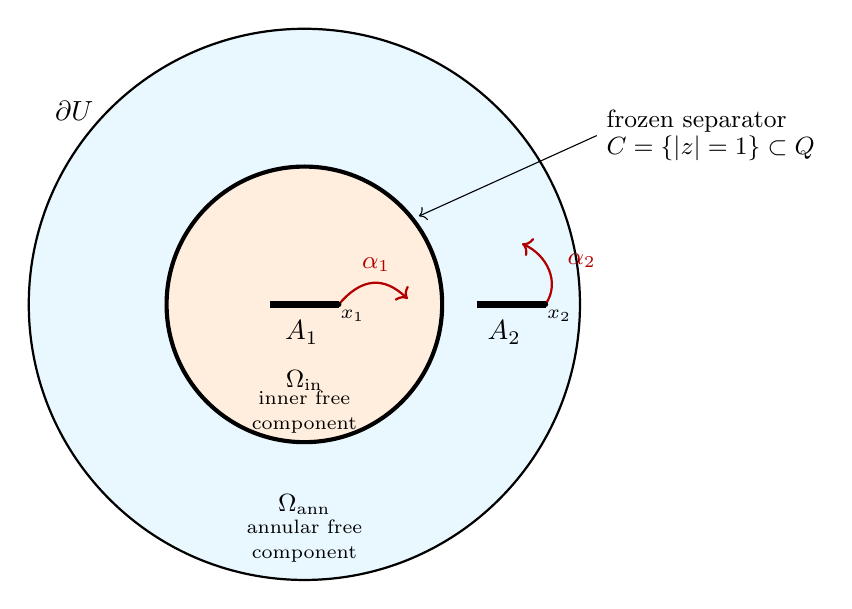
\begin{tikzpicture}[scale=1.75]
% free components, lightly shaded in different tints
\fill[cyan!9,even odd rule] (0,0) circle (2) (0,0) circle (1);
\fill[orange!13] (0,0) circle (1);
% localization boundary
\draw[thick] (0,0) circle (2);
\node at (140:2.18) {$\partial U$};
% the frozen separator, drawn bold
\draw[line width=1.5pt] (0,0) circle (1);
\draw[<-,shorten <=1.5pt] (38:1.02) -- (30:2.45)
  node[right,align=left] {\small frozen separator\\[-2pt]\small $C=\{|z|=1\}\subset Q$};
% atoms
\draw[line width=2.6pt] (-0.25,0) -- (0.25,0);
\node[below] at (-0.02,-0.05) {$A_1$};
\draw[line width=2.6pt] (1.25,0) -- (1.75,0);
\node[below] at (1.45,-0.05) {$A_2$};
% port arcs, one inside each free component
\draw[->,thick,red!70!black] (0.25,0) .. controls (0.42,0.20) and (0.58,0.20) .. (0.75,0.04);
\node[above,red!70!black] at (0.52,0.17) {\small $\alpha_1$};
\fill (0.25,0) circle (0.55pt);
\node[below right,inner sep=1pt] at (0.24,-0.02) {\scriptsize $x_1$};
\draw[->,thick,red!70!black] (1.75,0) .. controls (1.86,0.16) and (1.76,0.36) .. (1.58,0.44);
\node[right,red!70!black] at (1.84,0.32) {\small $\alpha_2$};
\fill (1.75,0) circle (0.55pt);
\node[below right,inner sep=1pt] at (1.74,-0.02) {\scriptsize $x_2$};
% component labels
\node at (0,-0.55) {\small $\Omega_{\mathrm{in}}$};
\node[align=center] at (0,-0.78) {\scriptsize inner free\\[-3pt]\scriptsize component};
\node at (0,-1.45) {\small $\Omega_{\mathrm{ann}}$};
\node[align=center] at (0,-1.72) {\scriptsize annular free\\[-3pt]\scriptsize component};
\end{tikzpicture}
\caption{The separation example of Example~\ref{ex:no-common-component}. The Jordan
localization is the disk $U=\{|z|<2\}$; the frozen inventory consists of the two atoms
$A_1=[-\frac14,\frac14]$ and $A_2=[\frac54,\frac74]$ and the bold circle $C$, a
frozen separator belonging to $Q$. The free domain $\Omfree=U\setminus Q$ has
exactly two components, shaded in different tints: the inner component
$\Omega_{\mathrm{in}}$ and the annular component $\Omega_{\mathrm{ann}}$. Each atom has
a singleton port arc ($\alpha_1$, $\alpha_2$) into its own component, so every
individual-access audit passes; but no single component ports to both atoms, so by
Theorem~\ref{thm:free-component} no protected ribbon-routing certificate exists, and by
the persistence clause no monotone connector enlargement inside $U$ can repair the
failure while $C$ stays in the frozen inventory.}
\label{fig:separation}
\end{figure}
% ---- end D:criterion ----

% ---- begin E:packets ----
% Cluster E, part 1: augmented atoms and the common-domain theorem
% Body-only LaTeX; uses only preamble macros and fixed cross-cluster labels.

\section{Augmented atoms and the common domain}\label{sec:packets}

The free-component criterion of Theorem~\ref{thm:free-component} is exact, and its
persistence clause makes failures permanent; but as a \emph{positive} test it is
expensive. Deciding whether one component of $\Omfree$ reaches every required atom
demands a global analysis of how each of the finitely many collars, obstacles, and
exclusions of the frozen inventory sits relative to all of the others, and
Example~\ref{ex:no-common-component} shows that no atom-by-atom inspection can
substitute for that analysis: individual accessibility of every atom is compatible
with an unrepairable separation. From a \emph{partial} package --- the situation in
which the criterion would actually be invoked, with the inventory delivered piecemeal
by an ambient proof program --- the exact free-domain test is therefore difficult to
verify directly \cite{MWman}.

The present section proves a sufficient criterion that is \emph{source-checkable}:
each of its clauses is verified against named, finite source data rather than against
the component structure of an open set. The idea is to reverse the direction of the
analysis. Instead of asking how the frozen set $Q$ decomposes the localization, we
package $Q$ itself into finitely many pairwise disjoint full continua --- each atom
augmented by the inventory pieces assigned to it, the remainder grouped into
separated-obstacle packets --- while reserving one free port for each original atom.
Once the completed packages are pairwise disjoint, sphere duality forces their common
complement to be \emph{connected}; connectedness, not component bookkeeping, then
delivers the common free component that Theorem~\ref{thm:free-component} demands.

The section has three parts. Definition~\ref{def:packet} fixes the packet structure
and its typed assignment record; Lemma~\ref{lem:packets} is the duality argument; and
Theorem~\ref{thm:common-domain} assembles the sufficient criterion. How the completed
packets are actually computed from raw assigned pieces, and how their defining clauses
are audited with persistent failure certificates, is the subject of
Section~\ref{sec:audit}; Example~\ref{ex:merger} there shows why the audit must be run
on the completions and not on the raw pieces.

\subsection{Filled hulls and augmented packets}\label{subsec:E-packet-def}

Recall from Section~\ref{sec:prelim} the filled hull of a compact plane set $K$:
\begin{equation}\label{eq:E-fill}
\Fill(K)\;=\;K\,\cup\,\bigcup\bigl\{\,B : B\ \text{a bounded component of}\
\C\setminus K\,\bigr\}
\end{equation}
(equation~(9.5) of \cite{MWman}). Since $K$ is compact, $\C\setminus K$ has exactly
one unbounded component $\Omega_\infty(K)$, and \eqref{eq:E-fill} says
\[
\Fill(K)\;=\;\C\setminus\Omega_\infty(K).
\]
Consequently $\Fill(K)$ is closed, and it is bounded because every closed round disk
containing $K$ has its exterior inside $\Omega_\infty(K)$; thus $\Fill(K)$ is compact.
Its complement is the single connected set $\Omega_\infty(K)$, so $\Fill(K)$ is
\emph{full}, and it is the smallest full compact set containing $K$: if $F\supset K$
is full and compact, then $\C\setminus F$ is a connected unbounded subset of
$\C\setminus K$, hence contained in $\Omega_\infty(K)$, which gives
$\Fill(K)\subset F$ after taking complements. Finally, if $K$ is a continuum, then so
is $\Fill(K)$: every bounded component $B$ of $\C\setminus K$ has
$\partial B\subset K$, so its closure $\overline B$ is a connected set meeting $K$,
and $\Fill(K)=K\cup\bigcup\overline B$ is a union of connected sets all meeting the
connected set $K$. The passage from $K$ to $\Fill(K)$ is what the manuscript calls
\emph{fullification}; its algebra --- and in particular the fact that interleaved
adjoin-and-fill operations compute a well-defined completion --- is developed in
Section~\ref{sec:audit}.

Throughout, the \emph{atoms} $A_1,\dots,A_s\Subset U$ are the pairwise disjoint full
continua of Section~\ref{sec:certificates} that the connector must join, and $Q$ is
the frozen set of Section~\ref{sec:criterion} (equation~(9.4) of \cite{MWman}): the
union of the atoms, the closed terminal protected collars, the separated obstacles,
the critical-value exclusion, and the localization-forbidden set, fixed once and for
all before any connector is chosen.

\begin{definition}[Augmented-atom packet; manuscript Definition 10.9]\label{def:packet}
For the frozen set $Q$, an \emph{augmented-atom packet} consists of full continua
\[
\widehat A_1,\dots,\widehat A_s,\
\widehat O_1,\dots,\widehat O_t\;\Subset\;U
\]
and pairwise disjoint port arcs $\alpha_i\colon[0,1]\to U$ such that:
\begin{enumerate}
\item every protected collar, obstacle, critical exclusion, and other component of
$Q$ has one typed assignment, either to a connected atom seed $A_i\cup E_i$ or to a
connected separated-obstacle seed $O_\ell$;
\item $\widehat A_i=\Fill(A_i\cup E_i)$ for every $i$, and
$\widehat O_\ell=\Fill(O_\ell)$ for every $\ell$;
\item the completed packets
$\widehat A_1,\dots,\widehat A_s,\widehat O_1,\dots,\widehat O_t$ are pairwise
disjoint and cover $Q$; and
\item $\alpha_i(0)=x_i\in A_i$, $\alpha_i\cap\widehat A_i=\{x_i\}$, and
\[
\alpha_i\bigl((0,1]\bigr)\;\subset\;
U\setminus\Bigl(\bigcup_{k}\widehat A_k\cup\bigcup_{\ell}\widehat O_\ell\Bigr),
\]
and $x_i$ is not the impression of a protected chain.
\end{enumerate}
The assignment records the component name, the proof-use stages, the attachment
trace, the return word, the selected sheet, and the absorb-or-separate decision.
\end{definition}

Some commentary on the four clauses. In clause~(1), $E_i$ denotes the union of the
inventory pieces assigned to the $i$-th atom; it may be empty, and the clause demands
that the resulting \emph{atom seed} $A_i\cup E_i$ be connected, so that an assigned
piece disjoint from its atom must be accompanied by connecting material assigned to
the same label. The assignment is \emph{typed}: it is a function from the finitely
many named constituents of the frozen inventory to the packet labels, and each
assigned piece carries the six recorded fields listed after clause~(4). Those fields
--- which component of the ambient package the piece is, at which proof-use stages it
is read, its attachment trace, its return word, its selected sheet, and whether the
decision taken for it was absorption or separation --- are bookkeeping data of the
ambient proof program; the planar topology of this section reads only the geometry of
the seeds. The record is nevertheless load-bearing: it is what makes a later change
of assignment an explicit, auditable re-decision rather than a silent repair, a point
Example~\ref{ex:merger} makes concrete.

In clause~(2), fullness of the completed packets is automatic: the seeds are compact
and connected, so their filled hulls are full continua by the discussion following
\eqref{eq:E-fill}. Clause~(3) is the substantive geometric hypothesis, and it is
stated for the \emph{completed} packets $\widehat A_i,\widehat O_\ell$, not for the
raw seeds: fullification can create intersections that the seeds do not have, and an
audit run at seed level certifies nothing (Example~\ref{ex:merger}). Coverage of $Q$
means that every item of the frozen inventory lies inside some completed packet, so
that outside the packets there is no frozen material at all --- this is the inclusion
that will place the common complement inside $\Omfree$. Clause~(4) is the port
clause. It is deliberately stronger than the port clause of
Definition~\ref{def:certificate}: the arc's positive-parameter part must avoid every
completed hull, whereas the arcs of Definition~\ref{def:certificate} avoid only the
obstacle set, the atoms, and the terminal collar tails, and the arc here must meet
even its own augmented atom $\widehat A_i$ only at the landing point $x_i$. The final requirement,
that $x_i$ not be the impression of a protected chain, keeps the port compatible with
the protected marking; it reappears in Section~\ref{sec:audit} as the requirement
that $x_i$ lie in the unprotected exposure locus, outside the forbidden impression
set $P_i$.

\subsection{Nonseparation of finite disjoint full families}\label{subsec:E-duality}

The engine of the common-domain theorem is a nonseparation statement for finitely
many disjoint full continua on the sphere. Here a compact set $K\subset S^2$ is
called full when $S^2\setminus K$ is connected; for a compact subset of the plane
this agrees with the planar notion, because adjoining the point at infinity to the
unbounded complementary component does not change connectivity, so a plane-full
compact set is sphere-full and conversely. The proof uses the compacta form of
Alexander duality \cite[pp.~256--257]{Hat02}:
\begin{equation}\label{eq:E-duality}
\widetilde H_0\bigl(S^2\setminus K;\Z\bigr)\;\cong\;\check H^1(K;\Z)
\end{equation}
for an arbitrary nonempty proper compact subset $K\subset S^2$ (equation~(9.6) of
\cite{MWman}). The \v{C}ech form, rather than the locally contractible special case,
is required here: the atoms and the assigned inventory pieces are arbitrary continua,
no local connectivity is assumed anywhere in this paper, and for such compacta
singular cohomology need not compute the group on the right of
\eqref{eq:E-duality}.

\begin{remark}\label{rem:E-cech}
The insistence on the \v{C}ech form is not pedantry but a structural feature of the
framework. Clause~(6) of Theorem~\ref{thm:realization} promises that no local
connectivity of any atom is ever required, and the packets of
Definition~\ref{def:packet} inherit whatever boundary pathology their atoms and
assigned pieces possess. \v{C}ech cohomology is the invariant that remains dual to
the complement's component count for every compact subset of the sphere, without any
tameness hypothesis; every duality argument below is stated so that it factors
through \eqref{eq:E-duality} alone.
\end{remark}

\begin{lemma}[Finite disjoint full packets; manuscript Lemma 10.10]\label{lem:packets}
If $K_0,\dots,K_N\subset S^2$ are pairwise disjoint nonempty full continua, then
\[
S^2\setminus\bigcup_{r=0}^{N}K_r
\]
is connected.
\end{lemma}

\begin{proof}
Write $X:=\bigcup_{r=0}^{N}K_r$. We may assume that $X$ is a proper subset of
$S^2$, so that \eqref{eq:E-duality} applies to $X$ and to each $K_r$: were $X=S^2$,
the sets $K_0,\dots,K_N$ would be finitely many pairwise disjoint nonempty closed
sets covering $S^2$; each would then be open as well, being the complement of the
union of the others, and connectedness of $S^2$ would force $N=0$ and $K_0=S^2$, in
which case the complement is empty and there is nothing to prove.

\emph{Step 1: each packet has vanishing first \v{C}ech cohomology.}
Fix $r$. Fullness of $K_r$ makes $S^2\setminus K_r$ connected, and it is nonempty
because $K_r$ is proper. Being open in $S^2$, the complement is locally path
connected, so connectedness makes it path connected and its reduced zeroth singular
homology vanishes. Hence \eqref{eq:E-duality}, applied to the nonempty proper
compact set $K_r$, gives
\[
\check H^1(K_r;\Z)\;\cong\;\widetilde H_0\bigl(S^2\setminus K_r;\Z\bigr)\;=\;0 .
\]

\emph{Step 2: disjoint neighborhoods split fine covers.}
The sets $K_0,\dots,K_N$ are finitely many pairwise disjoint compacta, so their
mutual distances in the spherical metric are positive; choose $\varepsilon>0$ smaller
than half the minimum of these distances and let $N_r$ be the open
$\varepsilon$-neighborhood of $K_r$. The $N_r$ are pairwise disjoint open sets with
$K_r\subset N_r$.

Call a cover of $X$ by relatively open subsets \emph{fine} when every member is
contained in one of the sets $N_r$. The fine covers are cofinal among all relatively
open covers of $X$: an arbitrary cover $\mathcal U$ is refined by the fine cover
$\{\,V\cap N_r : V\in\mathcal U,\ 0\le r\le N\,\}$, since
$X\subset\bigcup_rN_r$. Let $\mathcal V$ be a fine cover with nonempty members. Each
member lies in exactly one $N_r$, because the $N_r$ are pairwise disjoint; write
$\mathcal V_r$ for the members contained in $N_r$. Since
$X\cap N_r=K_r$, the collection $\mathcal V_r$ is a relatively open cover of $K_r$.
Two members taken from distinct collections $\mathcal V_r,\mathcal V_{r'}$ are
disjoint, lying in the disjoint sets $N_r,N_{r'}$; hence no simplex of the nerve of
$\mathcal V$ mixes the collections, and the nerve of $\mathcal V$ is the disjoint
union of the nerves of $\mathcal V_0,\dots,\mathcal V_N$. Simplicial cohomology of a
finite disjoint union is the direct sum, so
\[
H^1\bigl(\mathrm{nerve}\,\mathcal V;\Z\bigr)\;\cong\;
\bigoplus_{r=0}^{N}H^1\bigl(\mathrm{nerve}\,\mathcal V_r;\Z\bigr).
\]

\emph{Step 3: pass to the direct limit.}
\v{C}ech cohomology of $X$ is the direct limit of the nerve cohomologies over the
directed system of relatively open covers, and the fine covers are cofinal in that
system, so the limit may be computed over fine covers only. A refinement of a fine
cover is again fine after intersecting with the $N_r$, and its restriction to $N_r$
refines $\mathcal V_r$; the splitting of Step~2 is therefore compatible with the
refinement maps, and restriction to $N_r$ is cofinal among the covers of $K_r$
because any relatively open cover of $K_r$ extends to a fine cover of $X$ by
adjoining covers of the other packets. Since a direct limit commutes with the finite
direct sum, Step~1 gives
\[
\check H^1(X;\Z)\;\cong\;\bigoplus_{r=0}^{N}\check H^1(K_r;\Z)\;=\;0 .
\]

\emph{Step 4: apply duality a second time.}
The set $X$ is compact, nonempty, and proper, so \eqref{eq:E-duality} applies to $X$
itself:
\[
\widetilde H_0\bigl(S^2\setminus X;\Z\bigr)\;\cong\;\check H^1(X;\Z)\;=\;0 .
\]
The complement $S^2\setminus X$ is nonempty, and a nonempty space with vanishing
reduced zeroth homology is connected. This is the assertion.
\end{proof}

Lemma~\ref{lem:packets} is the disjoint counterpart of
Lemma~\ref{lem:tree-full}. There, unions of nonseparating continua meeting in
connected singletons were handled by the Janiszewski separation lemma, one attachment
at a time; here the continua are pairwise disjoint, the count is arbitrary, and the
duality argument dispenses with any hypothesis on how the packets face one another.
Nothing is assumed about the boundaries of the $K_r$ --- they may be nowhere locally
connected --- and no width, diameter, or separation estimate enters.

\subsection{The common-domain theorem}\label{subsec:E-common}

\begin{theorem}[Augmented-Atom Common-Domain Theorem; manuscript Theorem
10.11]\label{thm:common-domain}
Every augmented-atom packet determines one component of $\Omfree$ with simultaneous
singleton ports to every original atom. Hence it supplies a protected regulated
connector.
\end{theorem}

\begin{proof}
Let an augmented-atom packet be given, with completed packets
$\widehat A_1,\dots,\widehat A_s,\widehat O_1,\dots,\widehat O_t\Subset U$ and port
arcs $\alpha_1,\dots,\alpha_s$ as in Definition~\ref{def:packet}.

\emph{The exterior packet.}
Adjoin to the family the set
\[
K_0\;:=\;S^2\setminus U .
\]
The Jordan-disk hypothesis makes $K_0$ a full continuum: by the Jordan--Schoenflies
theorem the Jordan curve $\partial U$ divides the sphere into two open Jordan disks
with common boundary $\partial U$, the closure of the one containing $\infty$ is the
closed Jordan disk $S^2\setminus U$, hence a continuum, and its complement is the
connected set $U$, so $K_0$ is full in the sphere sense used in
Lemma~\ref{lem:packets}. Each completed packet is a plane-full continuum, hence
sphere-full as noted in Section~\ref{subsec:E-duality}, and compact containment
$\widehat A_i,\widehat O_\ell\Subset U$ makes every completed packet disjoint from
$K_0$; together with clause~(3) of Definition~\ref{def:packet}, the family
\[
K_0,\ \widehat A_1,\dots,\widehat A_s,\ \widehat O_1,\dots,\widehat O_t
\]
consists of $1+s+t$ pairwise disjoint nonempty full continua in $S^2$.

\emph{The augmented complement is connected.}
Lemma~\ref{lem:packets} applies to this family and makes its common complement
connected. Since $S^2\setminus K_0=U$, that complement is
\begin{equation}\label{eq:E-omega-aug}
\Omega_{\mathrm{aug}}\;:=\;
U\setminus\Bigl(\bigcup_{i}\widehat A_i\cup\bigcup_{\ell}\widehat O_\ell\Bigr)
\;=\;S^2\setminus\Bigl(K_0\cup\bigcup_i\widehat A_i\cup
\bigcup_\ell\widehat O_\ell\Bigr),
\end{equation}
a connected subset of $\C$, open because $U$ is open and the packets are compact. It
is nonempty: clause~(4) places the positive-parameter part of each port arc inside
it.

\emph{The augmented complement lies in one free component.}
Clause~(3) of Definition~\ref{def:packet} makes the completed packets cover $Q$, so
\[
\Omega_{\mathrm{aug}}
\;=\;U\setminus\Bigl(\bigcup_i\widehat A_i\cup\bigcup_\ell\widehat O_\ell\Bigr)
\;\subset\;U\setminus Q\;=\;\Omfree .
\]
A nonempty connected subset of the open set $\Omfree$ lies in exactly one of its
components; let $\Omega_0$ be the component containing $\Omega_{\mathrm{aug}}$. This
is the component that the packet determines.

\emph{The ports are simultaneous singleton ports of $\Omega_0$.}
By clause~(4), each port interior satisfies
\[
\alpha_i\bigl((0,1]\bigr)\;\subset\;
U\setminus\Bigl(\bigcup_k\widehat A_k\cup\bigcup_\ell\widehat O_\ell\Bigr)
\;=\;\Omega_{\mathrm{aug}}\;\subset\;\Omega_0 .
\]
Moreover $A_i\subset A_i\cup E_i\subset\widehat A_i$, so
\[
\alpha_i\cap A_i\;\subset\;\alpha_i\cap\widehat A_i\;=\;\{x_i\},
\]
and $x_i=\alpha_i(0)\in A_i$ gives $\alpha_i\cap A_i=\{x_i\}$: the arc meets its atom
exactly in the one free point $x_i$. The arcs are pairwise disjoint Jordan arcs by
Definition~\ref{def:packet}. Thus $\Omega_0$ has simultaneous singleton ports to
every original atom, in the sense of Section~\ref{sec:criterion}.

\emph{Conclusion.}
Theorem~\ref{thm:free-component} converts the simultaneous singleton ports of
$\Omega_0$ into a protected ribbon-routing certificate, and
Theorem~\ref{thm:realization} realizes that certificate by a compact connected full
carrier with singleton attachment traces, protected crosscut survival, and preserved
cyclic order. The packet therefore supplies a protected regulated connector.
\end{proof}

\begin{remark}\label{rem:E-common-domain}
Three remarks of the manuscript \cite{MWman} deserve emphasis. First, no local
connectivity or width estimate occurs anywhere in the argument: the packets may have
arbitrarily wild boundaries, the duality step of Lemma~\ref{lem:packets} is
insensitive to them, and no modulus, diameter, or incidence bound is invoked at any
point. Second, the construction is natural under an orientation-preserving conformal
homeomorphism of Jordan disks: the boundary extensions can be glued to a sphere
homeomorphism, and such a map carries filled packets to filled packets, ports to
ports, the common domain \eqref{eq:E-omega-aug} to the corresponding common domain,
and any selected connector to a connector for the transported data, exactly as in
Proposition~\ref{prop:naturality}; the commutation of such a sphere homeomorphism
with the operator $\Fill$ is proved in detail in the naturality paragraph of
Theorem~\ref{thm:audit}. Third, the spanning tree produced inside the common
component is not claimed canonical: Theorem~\ref{thm:free-component} supplies
\emph{some} embedded tree through the free component, and different choices give
different carriers with the same protected marking. Only the component $\Omega_0$,
the ports, and the survival data are determined by the packet.
\end{remark}

Theorem~\ref{thm:common-domain} consumes completed packets: it presupposes that the
filled hulls $\widehat A_i,\widehat O_\ell$ have already been computed from the typed
assignment and checked against clauses~(1)--(4). In practice the assignment delivers
raw pieces one at a time, and both the computation of the completions and the
verification of the clauses raise questions of their own --- whether the result
depends on the order of processing, and whether individually verified ports must be
untangled globally. The next section resolves both questions and equips the
verification with persistent failure certificates.
% ---- end E:packets ----

% ---- begin E:audit ----
% Cluster E, part 2: fixed-packet closure, persistent witnesses, port audit,
% the post-fullification merger example, and the cellwise certificate.
% Body-only LaTeX; uses only preamble macros and fixed cross-cluster labels.

\section{Fixed-packet closure and the port audit}\label{sec:audit}

Theorem~\ref{thm:common-domain} consumes completed packets, and its hypotheses leave
two apparent degrees of freedom in producing them. The first is a processing order.
The typed assignment of Definition~\ref{def:packet} delivers each packet as a finite
list of compact pieces, and a completion built incrementally --- adjoin a piece, fill,
adjoin the next piece carrying the same label, fill again --- seems to depend on the
order in which the pieces arrive. The second is a global untangling. Clause~(4)
demands pairwise disjoint port arcs avoiding every completed hull simultaneously,
whereas what an ambient proof program can realistically certify is one access arc per
atom, each verified in isolation; one might fear that the individual arcs must be
coordinated globally before they can serve together. This section proves that both
dependences are illusory once the typed assignment is fixed. Fullification is
order-independent (Lemma~\ref{lem:fill-absorption}); individual ports localize
simultaneously without any coordination (Lemma~\ref{lem:port-localization}); and the
resulting audit (Theorem~\ref{thm:audit}) characterizes the geometric packet clauses
by three checkable conditions whose failures are certified by witnesses that
\emph{persist} under every monotone same-label enlargement.
Example~\ref{ex:merger}, required by the structure of the theory, then shows that the
audit must be run on the completions and not on the raw seeds, and
Proposition~\ref{prop:cellwise} packages the whole verification into a cellwise
checklist.

\subsection{Order-independent fullification}\label{subsec:E-fill-algebra}

\begin{lemma}[Filled-hull absorption; manuscript Lemma 10.12]\label{lem:fill-absorption}
For compact plane sets $K,L$,
\begin{equation}\label{eq:E-absorption}
\Fill\bigl(\Fill(K)\cup L\bigr)\;=\;\Fill(K\cup L)
\end{equation}
(equation~(9.7) of \cite{MWman}). Consequently, sequentially adjoining and filling
finitely many compact pieces gives the filled hull of their union, independently of
processing order.
\end{lemma}

\begin{proof}
\emph{Step 1: the operator $\Fill$ is extensive, monotone, and idempotent.}
Extensivity, $K\subset\Fill(K)$, is immediate from the definition
\eqref{eq:E-fill}. For monotonicity, recall from Section~\ref{subsec:E-packet-def}
that
\[
\Fill(K)\;=\;\C\setminus\Omega_\infty(K),
\]
where $\Omega_\infty(K)$ is the unique unbounded component of $\C\setminus K$, and
that $\Fill(K)$ is compact. If $K\subset L$, then $\Omega_\infty(L)$ is a connected
unbounded subset of $\C\setminus L\subset\C\setminus K$, hence is contained in the
unique unbounded component of $\C\setminus K$:
\[
\Omega_\infty(L)\;\subset\;\Omega_\infty(K).
\]
Taking complements in $\C$ gives $\Fill(K)\subset\Fill(L)$. For idempotence, the
complement of $\Fill(K)$ is the single set $\Omega_\infty(K)$, which is connected and
unbounded; a compact set whose complement has exactly one component, an unbounded
one, has no bounded complementary components, so $\Fill(\Fill(K))=\Fill(K)$. We call
a compact set of the form $\Fill(M)$, equivalently a compact set equal to its own
filled hull, \emph{full}; by idempotence, $\Fill(K\cup L)$ is full.

\emph{Step 2: the two inclusions.}
Extensivity applied to the summand $K$ gives $K\cup L\subset\Fill(K)\cup L$, and
monotonicity then gives the first inclusion,
\[
\Fill(K\cup L)\;\subset\;\Fill\bigl(\Fill(K)\cup L\bigr).
\]
Conversely, monotonicity gives $\Fill(K)\subset\Fill(K\cup L)$, and extensivity gives
$L\subset K\cup L\subset\Fill(K\cup L)$; hence
\[
\Fill(K)\cup L\;\subset\;\Fill(K\cup L),
\]
and the set on the right is already full by Step~1. Applying $\Fill$ to this second
inclusion and using monotonicity and idempotence,
\[
\Fill\bigl(\Fill(K)\cup L\bigr)\;\subset\;\Fill\bigl(\Fill(K\cup L)\bigr)
\;=\;\Fill(K\cup L).
\]
The two displayed inclusions prove \eqref{eq:E-absorption}.

\emph{Step 3: finite order independence.}
Let $P_1,\dots,P_n$ be compact pieces and let $\pi$ be any permutation of
$\{1,\dots,n\}$. Define the incremental completions
\[
X_1:=\Fill\bigl(P_{\pi(1)}\bigr),
\qquad
X_j:=\Fill\bigl(X_{j-1}\cup P_{\pi(j)}\bigr)\quad(2\le j\le n).
\]
We claim $X_j=\Fill\bigl(P_{\pi(1)}\cup\dots\cup P_{\pi(j)}\bigr)$ for every $j$, by
induction. The base case is the definition of $X_1$. For the step, write
$K:=P_{\pi(1)}\cup\dots\cup P_{\pi(j-1)}$ and $L:=P_{\pi(j)}$; the inductive
hypothesis and \eqref{eq:E-absorption} give
\[
X_j=\Fill\bigl(\Fill(K)\cup L\bigr)=\Fill(K\cup L)
=\Fill\bigl(P_{\pi(1)}\cup\dots\cup P_{\pi(j)}\bigr).
\]
In particular $X_n=\Fill(P_1\cup\dots\cup P_n)$, which does not depend on $\pi$. The
same identity shows that filling may be interleaved arbitrarily, and even that two
partially completed runs of the same label may be merged: by
\eqref{eq:E-absorption} applied twice, once on each side of the union,
\[
\Fill\bigl(\Fill(K)\cup\Fill(L)\bigr)
=\Fill\bigl(K\cup\Fill(L)\bigr)
=\Fill(K\cup L)
\]
for all compact $K,L$. Every schedule of adjoin-and-fill operations on a fixed finite
set of pieces therefore computes the same completion.
\end{proof}

\subsection{Seeds, completions, and persistent witnesses}\label{subsec:E-witnesses}

For a fixed packet label $\ell$, let $S_\ell$ be the union of its original atom, when
present, and all compact pieces assigned to that label; $S_\ell$ is the \emph{raw
seed} of the packet. Its unique completion is
\begin{equation}\label{eq:E-completion}
K_\ell\;=\;\Fill(S_\ell)
\end{equation}
(equation~(9.8) of \cite{MWman}); by Lemma~\ref{lem:fill-absorption} this is what
every processing order computes. Note that when the label carries an atom, the
convention makes $A_i\subset S_i\subset K_i$.

Failures of the packet clauses are recorded by explicit geometric witnesses. For
$x\in K_\ell$, record its \emph{chamber},
\[
\mathrm{ch}_\ell(x)\;:=\;
\begin{cases}
\textsf{seed} & \text{if }x\in S_\ell,\\[2pt]
\text{the bounded component of }\C\setminus S_\ell\text{ containing }x
& \text{otherwise.}
\end{cases}
\]
A completed-packet merger then has the geometric witness
\begin{equation}\label{eq:E-witness}
\bigl(\ell,\ \ell',\ x,\ \mathrm{ch}_\ell(x),\ \mathrm{ch}_{\ell'}(x)\bigr),
\qquad x\in K_\ell\cap K_{\ell'}
\end{equation}
(display~(9.9) of \cite{MWman}): the tuple names the two colliding labels, a common
point, and, for each label, whether the point is seed material or lies in a named
bounded complementary chamber of the seed. Monotonicity of $\Fill$ shows that this
witness remains a merger after any same-label enlargement $S_\ell\subset S'_\ell$:
enlarging seeds enlarges completions, so
$x\in K_\ell\cap K_{\ell'}\subset K'_\ell\cap K'_{\ell'}$, and the same point
witnesses the merger of the enlarged packets. (The recorded chambers may upgrade ---
a bounded chamber of $S_\ell$ may be absorbed into the seed of $S'_\ell$, in which
case the record becomes \textsf{seed} --- but the intersection never empties.) The
same argument makes a \emph{localization escape}
\[
K_\ell\cap(\C\setminus U)\;\neq\;\varnothing
\]
persistent: a point of $K_\ell$ outside $U$ lies in $K'_\ell$ outside $U$ for every
same-label enlargement.

The third audited datum concerns ports. Let $P_i\subset A_i$ be the union of the
impressions forbidden by the protected marking at the last proof use; the protected
marking forbids exactly the impressions of the protected chains, so $P_i$ is the
union of those impressions inside $A_i$, and we use this identification in both
directions of the audit below. Define the
\emph{unprotected exposure locus}
\begin{equation}\label{eq:E-exposure}
\begin{aligned}
\Exp(A_i,K_i;P_i)\;=\;
\bigl\{\,x\in A_i\setminus P_i \;:\;{}&
\text{there is a Jordan arc }\gamma\colon[0,1]\to U\\
&\text{with }\gamma(0)=x
\text{ and }\gamma\cap K_i=\{x\}\,\bigr\}
\end{aligned}
\end{equation}
(display~(9.10) of \cite{MWman}). This is actual access data; boundary membership
alone is not substituted for \eqref{eq:E-exposure}. The distinction matters
precisely because no local connectivity is assumed: a point of
$\partial K_i\setminus P_i$ need not be the landing point of any arc --- the
boundary of a full continuum can consist almost entirely of non-accessible points
\cite{Pom92} --- so \eqref{eq:E-exposure} is an existence statement about arcs, and
it is this statement, not membership in a boundary set, that every clause below
reads.

\subsection{Simultaneous localization of individual ports}\label{subsec:E-localization}

\begin{lemma}[Individual ports localize simultaneously; manuscript Lemma
10.13]\label{lem:port-localization}
Suppose the completed atom packets $K_1,\dots,K_s\Subset U$ and obstacle packets
$L_1,\dots,L_t\Subset U$ form a pairwise disjoint family and
$\Exp(A_i,K_i;P_i)\neq\varnothing$ for every original atom. Then the access arcs can
be chosen pairwise disjoint, with positive-parameter parts in
\[
U\setminus\Bigl(\bigcup_{i}K_i\cup\bigcup_{\ell}L_\ell\Bigr).
\]
If $K_i\subset K_i'$, then
\begin{equation}\label{eq:E-exposure-monotone}
\Exp(A_i,K_i';P_i)\;\subset\;\Exp(A_i,K_i;P_i)
\end{equation}
(display~(9.11) of \cite{MWman}).
\end{lemma}

\begin{proof}
\emph{Disjoint localization neighborhoods.}
The family $K_1,\dots,K_s,L_1,\dots,L_t$ consists of finitely many pairwise disjoint
compacta, each compactly contained in the open set $U$. Their mutual distances are
positive, and so is the distance from each to $\C\setminus U$. Choose
$\varepsilon>0$ smaller than half the minimum of all these distances, and let $N_i$
be the open $\varepsilon$-neighborhood of $K_i$. Then $N_1,\dots,N_s$ are pairwise
disjoint open sets, each compactly contained in $U$, each containing its $K_i$, and
each missing every obstacle packet $L_\ell$ and every other atom packet $K_j$
($j\neq i$).

\emph{Localizing one arc.}
Fix $i$ and choose, by hypothesis, a point $x_i\in\Exp(A_i,K_i;P_i)$ together with a
Jordan arc $\gamma_i\colon[0,1]\to U$ from \eqref{eq:E-exposure}:
$\gamma_i(0)=x_i$ and $\gamma_i\cap K_i=\{x_i\}$. The landing point satisfies
$x_i\in A_i\subset K_i\subset N_i$, and $N_i$ is open, so continuity of $\gamma_i$ at
$0$ supplies $t_i\in(0,1]$ with $\gamma_i([0,t_i])\subset N_i$. Replace $\gamma_i$ by
its initial subarc $\gamma_i|_{[0,t_i]}$, reparametrized over $[0,1]$ and still
denoted $\gamma_i$. Restriction can only shrink the intersection with $K_i$ while
retaining the landing point, so the restricted arc still satisfies
$\gamma_i\cap K_i=\{x_i\}$, and its image now lies in $N_i$.

\emph{Simultaneity for free.}
The restricted arcs are pairwise disjoint because the $N_i$ are, and no coordination
between the choices was needed: each arc was shortened using only its own
neighborhood. Each positive-parameter part satisfies
\[
\gamma_i\bigl((0,1]\bigr)\;\subset\;N_i\setminus K_i,
\]
which misses $K_i$ by the singleton-intersection clause and misses every other packet
because $N_i$ does; hence it lies in
$U\setminus(\bigcup_iK_i\cup\bigcup_\ell L_\ell)$, as asserted.

\emph{Monotonicity.}
Let $K_i\subset K_i'$ and let $x\in\Exp(A_i,K_i';P_i)$, witnessed by an arc $\gamma$
with $\gamma(0)=x$ and $\gamma\cap K_i'=\{x\}$. Every arc avoiding the larger packet
off its landing point also avoids the smaller one: $\gamma\cap K_i\subset
\gamma\cap K_i'=\{x\}$, while $x\in A_i\subset K_i$ keeps $x$ in the intersection, so
$\gamma\cap K_i=\{x\}$ and the same arc witnesses $x\in\Exp(A_i,K_i;P_i)$. This
proves \eqref{eq:E-exposure-monotone}. In particular, an \emph{empty} exposure locus
stays empty under every same-label enlargement of the packet: port loss, once
incurred, is persistent.
\end{proof}

\subsection{The audit theorem}\label{subsec:E-audit-thm}

By the \emph{geometric augmented-packet clauses} of a fixed finite typed assignment
we mean clauses (1)--(4) of Definition~\ref{def:packet}, evaluated on the completions
determined by that assignment; the typed record itself --- component name, proof-use
stages, attachment trace, return word, selected sheet, absorb-or-separate decision
--- is data carried along unchanged, not a geometric assertion to be audited.

\begin{theorem}[Fixed-Packet Closure and Port Audit; manuscript Theorem
10.14]\label{thm:audit}
For a fixed finite typed assignment, the geometric augmented-packet clauses hold if
and only if:
\begin{enumerate}
\item the frozen inventory is covered and every raw seed $S_\ell$ is compact and
connected;
\item the unique completions $K_\ell=\Fill(S_\ell)$ are pairwise disjoint and
compactly contained in $U$; and
\item $\Exp(A_i,K_i;P_i)\neq\varnothing$ for every original atom: the
unprotected exposure locus is nonempty.
\end{enumerate}
The completions are independent of processing order. Merger, localization, and
empty-exposure defects persist under monotone same-label enlargement. The complete
audit is natural under a conformal homeomorphism of Jordan localizations that
transports the full packets and protected marking.
\end{theorem}

\begin{proof}
\emph{Closure.}
Lemma~\ref{lem:fill-absorption} gives unique, order-independent completions
$K_\ell=\Fill(S_\ell)$: every schedule of adjoin-and-fill operations on the pieces of
a label computes \eqref{eq:E-completion}. If clause~(1) holds, each raw seed is a
compact connected set, so each completion is a full continuum, by the discussion
following \eqref{eq:E-fill}.

\emph{Equivalence.}
Suppose first that clauses (1)--(3) hold. Clause~(1) is precisely clause~(1) of
Definition~\ref{def:packet}: the coverage assertion is common to both, and
connectedness of the raw seeds is the connectedness demanded of the atom seeds
$A_i\cup E_i$ and obstacle seeds $O_\ell$. Writing $\widehat A_i:=K_i$ for the atom
labels and $\widehat O_\ell:=L_\ell$ for the obstacle labels, clause~(2) of the
definition holds by \eqref{eq:E-completion}, and the sets are full continua by the
closure paragraph. Clause~(2) of the audit makes these completions pairwise disjoint
and, being compact subsets of the open set $U$, compactly contained in $U$; coverage
of $Q$ follows from clause~(1), since $Q\subset\bigcup_\ell S_\ell\subset
\bigcup_\ell K_\ell$. This is clause~(3) of the definition. Finally, clauses~(2)
and~(3) of the audit satisfy the hypotheses of
Lemma~\ref{lem:port-localization}, which produces pairwise disjoint Jordan arcs
$\alpha_i$ with $\alpha_i(0)=x_i\in A_i\setminus P_i$,
$\alpha_i\cap K_i=\{x_i\}$, and positive-parameter parts in the common complement
$U\setminus(\bigcup_kK_k\cup\bigcup_\ell L_\ell)$ --- exactly clause~(4) of the
definition, including its final requirement: $P_i$ contains every impression
forbidden by the protected marking, so $x_i\notin P_i$ is not the impression of a
protected chain.

Conversely, suppose the geometric packet clauses hold. Clause~(1) of the definition
is clause~(1) of the audit, as before. The completed packets of the definition are
the unique completions \eqref{eq:E-completion} of the assigned seeds, and clause~(3)
of the definition makes them pairwise disjoint, while
$\widehat A_i,\widehat O_\ell\Subset U$ gives compact containment: clause~(2) of the
audit. For clause~(3) of the audit, fix an atom $A_i$. The packet's own port arc
$\alpha_i$ satisfies $\alpha_i(0)=x_i\in A_i$, $\alpha_i\cap\widehat A_i=\{x_i\}$,
and maps into $U$; since $\widehat A_i=K_i$, the arc witnesses
$x_i\in\Exp(A_i,K_i;P_i)$ provided $x_i\notin P_i$, and this is the final requirement
of clause~(4): $x_i$ is not the impression of a protected chain, and $P_i$ consists
of such impressions. Hence the exposure locus is nonempty, completing the
equivalence.

\emph{Persistence.}
Monotonicity of $\Fill$ makes the merger witnesses \eqref{eq:E-witness} and the
localization-escape witnesses persistent under monotone same-label enlargement, as
recorded in Section~\ref{subsec:E-witnesses}: the witnessing point lies in the
enlarged completions and outside the unchanged localization, respectively. The
monotonicity clause \eqref{eq:E-exposure-monotone} of
Lemma~\ref{lem:port-localization} makes empty exposure persistent: the locus of the
enlarged packet is a subset of the old locus, so it cannot become nonempty by
enlargement. Thus each of the three defect types, once witnessed, is witnessed
forever along every monotone same-label enlargement of the seeds.

\emph{Naturality.}
Let $\varphi\colon U\to V$ be an orientation-preserving conformal homeomorphism of
Jordan localizations that transports the full packets and the protected marking. By
the Carath\'eodory extension theorem for Jordan domains \cite{Pom92}, $\varphi$
extends to a homeomorphism $\overline U\to\overline V$ of the closures; restricting
to the boundaries gives a homeomorphism $\partial U\to\partial V$ of Jordan curves.
The complementary sets $S^2\setminus U$ and $S^2\setminus V$ are closed Jordan disks,
and by the Schoenflies theorem \cite{New51} the boundary homeomorphism extends to a
homeomorphism between them; composing with a self-homeomorphism of the target disk
that is the identity on its boundary circle and moves the image of $\infty$ to
$\infty$, we may arrange that the extension fixes $\infty$. Gluing along
$\partial U$ yields a sphere homeomorphism $\Phi$ with $\Phi|_U=\varphi$ and
$\Phi(\infty)=\infty$. For any compact $K\subset\C$, the homeomorphism $\Phi$ carries
the components of $S^2\setminus K$ bijectively onto the components of
$S^2\setminus\Phi(K)$, and it carries the component containing $\infty$ to the
component containing $\infty$; deleting $\infty$, it carries the unbounded
complementary component of $K$ to the unbounded complementary component of
$\Phi(K)$, and the bounded components to the bounded components. Hence $\Phi$
commutes with $\Fill$:
\[
\Phi\bigl(\Fill(K)\bigr)\;=\;\Fill\bigl(\Phi(K)\bigr).
\]
Consequently $\Phi$ carries raw seeds to raw seeds (piece by piece, with the same
typed record), completions to completions, merger witnesses
\eqref{eq:E-witness} to merger witnesses (the point $x$ to $\Phi(x)$, the chambers to
the corresponding chambers, seed record to seed record), and localization escapes to
localization escapes: $\Phi(\C\setminus U)=\C\setminus V$, so a point of $K_\ell$
outside $U$ is carried to a point of the transported completion outside $V$. It also transports the port data: $P_i$ maps to
the transported forbidden impression set, and $\gamma\mapsto\Phi\circ\gamma$ is a
bijection between the arcs read by \eqref{eq:E-exposure} in $U$ and those read by the
transported locus in $V$, because $\Phi|_U=\varphi$ is a homeomorphism onto $V$ and
$\Phi(\gamma)\cap\Phi(K_i)=\Phi(\gamma\cap K_i)$. Each audit clause therefore holds
for the transported assignment if and only if it holds for the original: the
complete audit is natural.
\end{proof}

The theorem does not construct the typed assignment. What it proves is that, once
the assignment is fixed, a favorable completion order and a global untangling of
already existing individual ports are \emph{not} additional degrees of freedom: the
completions are canonical by Lemma~\ref{lem:fill-absorption}, and individual
exposure already implies simultaneous localized ports by
Lemma~\ref{lem:port-localization}. The one choice that matters --- which inventory
piece is assigned to which label --- is made upstream and recorded in the typed
data. The following example, the merger half of the required failure taxonomy, shows
that this choice genuinely matters, and that its defects surface only after
fullification.

\subsection{A post-fullification packet merger}\label{subsec:E-merger}

\begin{example}[Post-fullification packet merger]\label{ex:merger}
Work in the Jordan localization $U:=\{z\in\C:|z|<3\}$, and consider a two-packet
system whose typed assignment creates the raw seeds
\[
S_1\;:=\;\{z:|z|=1\},
\qquad
S_2\;:=\;\bigl[-\tfrac14,\tfrac14\bigr]\subset\mathbb R,
\]
say with both labels typed as separated obstacles recorded for future proof use.
Each seed is compact and connected, so clause~(1) of Theorem~\ref{thm:audit} holds,
and the seeds are pairwise \emph{disjoint}: every point of $S_1$ has modulus $1$,
every point of $S_2$ has modulus at most $\tfrac14$. Consequently every seed-level
disjointness audit passes --- any inspection of the raw pieces, in any processing
order, at any stage of the assignment, sees pairwise disjoint data.

The completions tell a different story. The segment has connected complement, so
\[
K_2\;=\;\Fill(S_2)\;=\;S_2 ,
\]
but the complement of the circle has exactly two components, the bounded open unit
disk and the unbounded set $\{|z|>1\}$, so
\[
K_1\;=\;\Fill(S_1)\;=\;\{z:|z|\le1\}\;\supset\;S_2 .
\]
Hence
\[
K_1\cap K_2\;\supset\;S_2\;\neq\;\varnothing
\]
(indeed $K_1\cap K_2=S_2$), and clause~(2) of Theorem~\ref{thm:audit} fails: the
merger appears only after fullification. The geometric witness \eqref{eq:E-witness}
at the point $x=0$ is
\[
\bigl(1,\ 2,\ 0,\ \mathrm{ch}_1(0),\ \mathrm{ch}_2(0)\bigr),
\qquad
\mathrm{ch}_1(0)=\{z:|z|<1\},
\quad
\mathrm{ch}_2(0)=\textsf{seed}:
\]
the origin is not seed material of label $1$ --- it lies in the recorded bounded
complementary chamber of $S_1$, the open unit disk --- while for label $2$ it lies in
the seed itself. See Figure~\ref{fig:merger}.

By monotonicity of $\Fill$, the witness persists under \emph{every} same-label
enlargement $S_\ell\subset S'_\ell$: the enlarged completions satisfy
$K_1\subset K'_1$ and $K_2\subset K'_2$, so $0\in K'_1\cap K'_2$ continues to
witness a merger. The persistence clause of Theorem~\ref{thm:audit} is therefore
sharp: the defect cannot be repaired by growing the seeds. What can remove it is
only a \emph{different typed assignment} --- for instance, assigning $S_2$ to
packet~$1$, together with, say, the connecting radius $[\tfrac14,1]$ so that the
label-$1$ seed $S_1\cup[\tfrac14,1]\cup S_2$ remains connected as clause~(1)
requires; the single completion is then the closed unit disk and no merger remains.
The typed record of Definition~\ref{def:packet} makes this an explicit
\emph{re-decision}, not a repair: the record of the segment changes its assignment,
and the change is visible in the audit trail. Within the fixed assignment, the
failure certificate is final.

This is exactly why clause~(3) of Definition~\ref{def:packet} requires disjointness
of the \emph{completed} packets, not of the raw seeds. Raw-seed disjointness is not
stable under fullification: an audit performed at seed level would certify the
present system and hand Theorem~\ref{thm:common-domain} a family that is not
pairwise disjoint, invalidating the duality argument of Lemma~\ref{lem:packets} at
its first step. Auditing the completions, by contrast, costs nothing extra ---
Lemma~\ref{lem:fill-absorption} makes the completions canonical --- and it converts
every failure into a persistent witness \eqref{eq:E-witness}.
\end{example}

\begin{figure}[t]
\centering
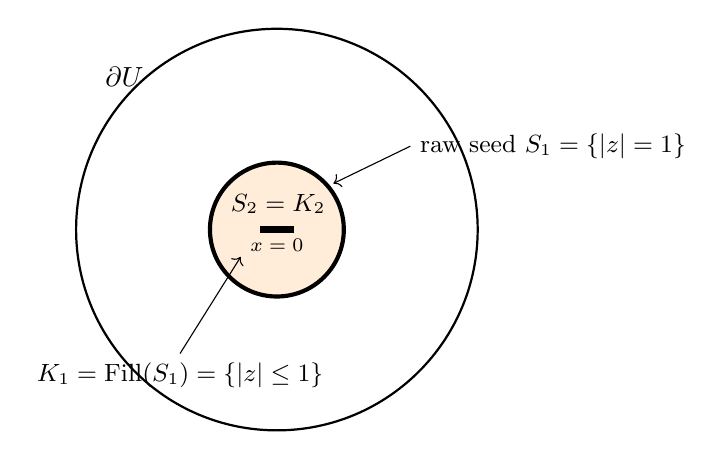
\begin{tikzpicture}[scale=0.85]
% localization boundary
\draw[thick] (0,0) circle (3);
\node at (135:3.22) {$\partial U$};
% filled hull K_1, shaded
\fill[orange!15] (0,0) circle (1);
% raw seed S_1
\draw[line width=1.5pt] (0,0) circle (1);
\draw[<-,shorten <=1.5pt] (40:1.03) -- (32:2.35)
  node[right,align=left] {\small raw seed $S_1=\{|z|=1\}$};
% shaded-hull annotation
\draw[<-,shorten <=1.5pt] (215:0.62) -- (232:2.35)
  node[below,align=left] {\small $K_1=\Fill(S_1)=\{|z|\le1\}$};
% raw seed S_2 inside the hull
\draw[line width=2.6pt] (-0.25,0) -- (0.25,0);
\node[above] at (0.02,0.09) {\small $S_2=K_2$};
% witness point
\fill (0,0) circle (1.3pt);
\node[below,inner sep=2pt] at (0,-0.05) {\scriptsize $x=0$};
\end{tikzpicture}
\caption{The post-fullification merger of Example~\ref{ex:merger} in the
localization $U=\{|z|<3\}$. The raw seeds --- the circle $S_1$ and the segment
$S_2$ --- are disjoint, so every seed-level disjointness audit passes. But the
completion $K_1=\Fill(S_1)$ is the closed unit disk (shaded), which contains
$S_2=K_2$: the completed packets merge. The witness point $x=0$ carries the record
$(1,2,0,\mathrm{ch}_1(0),\mathrm{ch}_2(0))$ with $\mathrm{ch}_1(0)$ the bounded
complementary chamber $\{|z|<1\}$ of $S_1$ and $\mathrm{ch}_2(0)=\textsf{seed}$. By
monotonicity of $\Fill$ the merger persists under every same-label enlargement of
the seeds; only a different typed assignment removes it.}
\label{fig:merger}
\end{figure}

\subsection{The cellwise certificate}\label{subsec:E-cellwise}

The audit clauses of Theorem~\ref{thm:audit} still require computing each completion
and comparing every pair of completions across the localization. The final result of
this section decomposes even this: it confines each packet to its own closed Jordan
cell, inside which the completion is trapped automatically and the port verification
becomes local to the cell. Disjointness of the completions then follows from
disjointness of the cells, which is checked on $N$ disks rather than on
$\binom N2$ pairs of filled hulls.

\begin{proposition}[Cellwise packet-and-port certificate; manuscript Proposition
10.15]\label{prop:cellwise}
Let $U$ be a Jordan domain and let $D_1,\dots,D_N\Subset U$ be pairwise disjoint
closed Jordan disks. Suppose every packet has a compact connected raw seed
$S_\ell\Subset D_\ell$, the seeds cover the complete frozen inventory, and every
original atom $A_i\subset S_i$ has an unprotected point $x_i\in A_i\setminus P_i$
and a Jordan arc $\gamma_i\colon[0,1]\to D_i$ satisfying
\begin{equation}\label{eq:E-arc-condition}
\gamma_i(0)=x_i,
\qquad
\gamma_i\bigl((0,1)\bigr)\subset D_i\setminus S_i,
\qquad
\gamma_i(1)\in\partial D_i
\end{equation}
(condition~(9.11a) of \cite{MWman}). Then $K_\ell=\Fill(S_\ell)\Subset D_\ell$, the
completed packets are pairwise disjoint, every $x_i\in\Exp(A_i,K_i;P_i)$, and the
packet system has simultaneous ports, one common free component, and a protected
regulated connector.
\end{proposition}

\begin{proof}
\emph{Step 1: the completion is trapped in its cell.}
Fix $\ell$. By the Schoenflies theorem, $S^2\setminus D_\ell$ is an open Jordan disk
containing $\infty$, so its planar part $\C\setminus D_\ell$ --- an open disk with
one point removed --- is connected, and it is unbounded. Since
$S_\ell\Subset D_\ell$ means $S_\ell\subset\Int D_\ell$, the exterior
$\C\setminus D_\ell$ is a connected unbounded subset of $\C\setminus S_\ell$ and
therefore lies in the unbounded component $\Omega_\infty(S_\ell)$. Consequently
every bounded component $B$ of $\C\setminus S_\ell$ is disjoint from
$\C\setminus D_\ell$ --- distinct components of $\C\setminus S_\ell$ are disjoint
--- so $B\subset D_\ell$, and $\Fill(S_\ell)\subset D_\ell$. The containment is
compact: a point $x\in\partial D_\ell$ does not lie in $S_\ell\subset\Int D_\ell$,
and every neighborhood of $x$ meets $\C\setminus D_\ell\subset
\Omega_\infty(S_\ell)$; since the component of $\C\setminus S_\ell$ containing $x$
is open and contains a small ball around $x$, that component meets
$\Omega_\infty(S_\ell)$ and hence equals it, so $x\in\Omega_\infty(S_\ell)$ and
$x\notin\Fill(S_\ell)$. Thus $K_\ell=\Fill(S_\ell)\subset\Int D_\ell$, and being
compact, $K_\ell\Subset D_\ell$. The cells are pairwise disjoint, so the completions
are pairwise disjoint, and $D_\ell\Subset U$ gives $K_\ell\Subset U$.

\emph{Step 2: the arc condition certifies exposure.}
Fix $i$. The point $\gamma_i(1)$ lies on the Jordan curve $\partial D_i$, which
bounds the closed Jordan disk $S^2\setminus\Int D_i$ containing $\infty$ in its
interior. Straightening this disk by the Schoenflies theorem \cite{New51} and taking
the preimage of a radius, we obtain a Jordan arc $\beta$ from $\gamma_i(1)$ to
$\infty$ meeting $D_i$ only at $\gamma_i(1)$. Consider the concatenated set
\[
\Gamma\;:=\;\gamma_i\bigl((0,1]\bigr)\,\cup\,\bigl(\beta\setminus\{\infty\}\bigr),
\]
a connected unbounded subset of $\C$. It is disjoint from $S_i$: the piece
$\gamma_i((0,1))$ lies in $D_i\setminus S_i$ by \eqref{eq:E-arc-condition}; the
point $\gamma_i(1)$ lies on $\partial D_i$, which misses $S_i\subset\Int D_i$; and
$\beta\setminus\{\gamma_i(1),\infty\}$ lies in $\C\setminus D_i\subset
\C\setminus S_i$. A connected unbounded subset of $\C\setminus S_i$ lies in the
unbounded component $\Omega_\infty(S_i)$, so in particular
\[
\gamma_i\bigl((0,1]\bigr)\;\subset\;\Omega_\infty(S_i)
\;=\;\C\setminus\Fill(S_i),
\]
that is, $\gamma_i((0,1])$ misses $K_i$. Since $x_i\in A_i\subset S_i\subset K_i$,
this gives
\[
\gamma_i\cap K_i\;=\;\{x_i\} .
\]
The arc $\gamma_i$ maps into $D_i\subset U$, and $x_i\in A_i\setminus P_i$ by
hypothesis, so $\gamma_i$ is precisely an arc of the form read by
\eqref{eq:E-exposure}: every $x_i\in\Exp(A_i,K_i;P_i)$.

\emph{Step 3: assembly.}
The three audit clauses of Theorem~\ref{thm:audit} now hold: clause~(1), because the
seeds are compact, connected, and cover the complete frozen inventory by hypothesis;
clause~(2), by Step~1; and clause~(3), by Step~2. Lemma~\ref{lem:port-localization}
turns the individual arcs into pairwise disjoint simultaneous port arcs with
positive-parameter parts in the common complement of the completions, and
Theorem~\ref{thm:audit} certifies that the geometric augmented-packet clauses of
Definition~\ref{def:packet} hold for this assignment. Theorem~\ref{thm:common-domain}
then determines one common free component of $\Omfree$ with simultaneous singleton
ports to every original atom and supplies a protected regulated connector.
\end{proof}

This proposition is sufficient only, and we close the section by marking the
boundary of what it proves, in the discipline of Section~\ref{sec:scope}. The
cellwise certificate solves the planar verification problem once the cells
$D_\ell$, the complete seeds $S_\ell$, and the unprotected arcs $\gamma_i$ are
supplied. The actual virtual theorem contemplated by the source manuscript must
still \emph{construct} those cells, complete seeds, and unprotected arcs, and must
transport them through the final Wave horizon; that construction is posed in
\cite{MWman} only as an open problem, it is not addressed by anything in this paper,
and no clause of Theorem~\ref{thm:audit} or Proposition~\ref{prop:cellwise} is
promoted here to a statement about virtual carriers, the Wave horizon, or Mandelbrot
local connectivity.
% ---- end E:audit ----

% ---- begin F:decoration ----
% Cluster F: the finite direct-decoration application (manuscript §10.11)
% Body-only LaTeX; preamble macros, theorem environments, and cite keys per CONVENTIONS.md.

\section{A finite direct-decoration application}\label{sec:decoration}

The certification framework of the preceding sections was assembled for a
purpose, and this final section is its intended consumer.  The setting is
the \emph{direct-decoration} configuration that the source manuscript
\cite{MWman} extracts from the decoration construction of Kahn and Lyubich
\cite{KL08}: a closed Jordan puzzle piece carrying two disjoint univalent
pullbacks of itself, iterated to produce a rooted binary tree of finite
pullback fibers accumulating on a Cantor family of end fibers.  The
resulting rooted-end compactum has \emph{infinitely many} components, so
the finite packet technology of Sections~\ref{sec:packets}
and~\ref{sec:audit} does not apply as it stands; the first task of this
section is to extend the nonseparation lemma to nested infinite packets
(Lemma~\ref{lem:nested-packets}).  The second task is geometric: the
inverse branches transport a single Jordan cell around the root continuum
into a \emph{gap-cell atlas}, a family of pairwise disjoint closed Jordan
cells, one around every finite fiber, each isolating its fiber from the
entire remaining compactum (Theorem~\ref{thm:gap-cells}).  The atlas is
precisely the dynamical realization of the cellwise criterion of
Proposition~\ref{prop:cellwise}: the cells that the cellwise certificate
asks the user to supply are here produced by the dynamics itself, at every
finite address simultaneously.  The final results assemble the package.
Packet replacement (Theorem~\ref{thm:packet-replacement}) shows that
fullifying finitely many selected fibers inside their cells preserves the
connected complement; the port lemma (Lemma~\ref{lem:impression-port})
shows that a proper compact set of protected impressions always leaves a
free port; and the protected-carrier theorem (Theorem~\ref{thm:carrier})
concludes that every finite selection of decoration addresses, decorated
with actual protected prime-end chains at the root, admits a protected
regulated connector in the sense of Theorem~\ref{thm:realization} that
avoids every unselected finite fiber and every end fiber and preserves the
transported prime ends with their cyclic order.  Throughout,
\emph{fullification} is the manuscript's term for the passage from a
compact set to its filled hull $\Fill(\,\cdot\,)$ of
Section~\ref{sec:packets}, and \emph{atom} retains the meaning fixed in
Section~\ref{sec:certificates}.

Every result of this section is reproduced, with notational streamlining
only, from Section~10.11 of the manuscript \cite{MWman}
(Lemma~10.39 through Theorem~10.45); the proofs are the manuscript's
proofs, expanded for readability.  One background result, the
direct-decoration pullback compactification (manuscript Theorem~10.37), is
\emph{quoted without proof}, and only three of its conclusions are used.
The section closes with the manuscript's own caveat on the strictly
finite, direct-scale reach of the application.

\subsection{The direct-decoration setting}\label{subsec:F-setting}

Following Section~10.11 of the manuscript \cite{MWman}, which organizes
dynamical data supplied by the decoration source of Kahn--Lyubich
\cite{KL08}, fix the following configuration.  Let $f$ be a polynomial
with
\[
K(f)=J(f),
\]
an assumption the manuscript makes explicitly, let $q\ge1$, and let $P$ be
a closed Jordan puzzle piece (in the manuscript's normalization,
$P=Y^{(n-1)q+1}$).  Put $g=f^{q}$ and let
\begin{equation}\label{eq:F-pullbacks}
g\colon Q_a\longrightarrow P,\qquad a\in\mathcal A:=\{0,1\},
\end{equation}
be the two \emph{actual univalent pullbacks} of $P$ inside $P$ (equation
(HT6) of \cite{MWman}).  Here $P$, $Q_0$, $Q_1$ are closed Jordan puzzle
pieces, the pullbacks satisfy $Q_0\cap Q_1=\varnothing$, and each proper
degree-one restriction extends to a homeomorphism of the \emph{closed}
pieces.  These closed-piece assertions---not merely disjointness of
interiors---are what the arguments below use, and the manuscript records
the separation argument for the closed pieces, which we reproduce.
Suppose $Q_0$ and $Q_1$ met at a point $z$.  Univalence of each
restriction makes $z$ a regular point of $g$, so $g$ is a local
homeomorphism at $z$; the local inverse defined on a small Jordan
half-neighborhood of $g(z)$ in $P$ would then belong to both pullback
components, contradicting their distinctness.  Hence
$Q_0\cap Q_1=\varnothing$ as closed sets, and proper degree one makes each
restriction $g\colon Q_a\to P$ a homeomorphism of closed Jordan pieces.
Write
\[
\phi_a\colon P\longrightarrow Q_a,\qquad a\in\mathcal A,
\]
for the two inverse branches; each is a homeomorphism of closed Jordan
pieces, conformal and orientation-preserving on the interior, with
$g\circ\phi_a=\id_P$.

Let $K_0\Subset\Int V_0$ be the \emph{terminal primitive root} of the
source construction: a filled Julia set, in particular a nondegenerate
full continuum.  The source construction makes $V_0$, $Q_0$, $Q_1$
distinct puzzle pieces of the common depth $nq+1$.  Their interiors are
pairwise disjoint, and $K_0$ is compactly contained in the interior of the
first; hence the \emph{root-gap relation}
\begin{equation}\label{eq:F-root-gap}
K_0\cap(Q_0\cup Q_1)=\varnothing
\end{equation}
(equation (HT7) of \cite{MWman}) holds, and the separation in
\eqref{eq:F-root-gap} is separation of \emph{closed} pieces.

\subsubsection*{Addresses, fibers, and the rooted-end compactum}
Let $\mathcal A^{<\mathbb N}$ denote the set of finite words in the
alphabet $\mathcal A=\{0,1\}$, including the empty word $\varepsilon$, and
let $\mathcal A^{\mathbb N}$ denote the set of infinite words.  For a
finite word $w=a_1\cdots a_m$ put
\begin{equation}\label{eq:F-words}
\phi_w=\phi_{a_1}\circ\cdots\circ\phi_{a_m},
\qquad
Q_w=\phi_w(P),
\qquad
K_w=\phi_w(K_0)
\end{equation}
(equation (HT8) of \cite{MWman}), with the conventions
$\phi_\varepsilon=\id_P$, $Q_\varepsilon=P$, and
$K_\varepsilon=K_0$.  For a one-letter word $a$ the cylinder $Q_a$ of
\eqref{eq:F-words} agrees with the pullback of \eqref{eq:F-pullbacks}, so
the notation is consistent; the root fiber is written $K_0$ throughout,
and the depth-one fibers are written $\phi_0(K_0)$, $\phi_1(K_0)$ with
explicit branches whenever a subscript could be misread as the root
label.  Each $\phi_w$ is a homeomorphism of $P$ onto the closed Jordan
piece $Q_w$, and $g^{|w|}\colon Q_w\to P$ is univalent.  For
$\omega\in\mathcal A^{\mathbb N}$, write $\omega|m$ for the initial
subword of length $m$ and define the \emph{end fiber}
\begin{equation}\label{eq:F-end-fiber}
E_\omega=\bigcap_{m\ge1}Q_{\omega|m}
\end{equation}
(equation (HT9) of \cite{MWman}).

Three combinatorial consequences of the standing data are used
repeatedly, and we record them once with their one-line proofs.
\emph{Nesting under extension}: appending a symbol descends one level,
\[
Q_{wa}=\phi_w\bigl(\phi_a(P)\bigr)=\phi_w(Q_a)\subset\phi_w(P)=Q_w ,
\]
so each $E_\omega$ in \eqref{eq:F-end-fiber} is a nested intersection of
nonempty compact connected sets, hence a nonempty compact connected set.
\emph{Incomparable words have disjoint cylinders}: if neither of $u,v$ is
a prefix of the other, write $u=pas$, $v=pbt$ with $p$ the longest common
prefix and $a\ne b$; then $Q_u\subset\phi_p(Q_a)$ and
$Q_v\subset\phi_p(Q_b)$, and injectivity of $\phi_p$ together with
$Q_0\cap Q_1=\varnothing$ gives $Q_u\cap Q_v=\varnothing$.
\emph{The root gap pulls back}: for every finite word $u$, applying the
injective map $\phi_u$ to \eqref{eq:F-root-gap} gives
\begin{equation}\label{eq:F-root-gap-pullback}
K_u\cap(Q_{u0}\cup Q_{u1})=\varnothing ,
\end{equation}
so every finite fiber lies in the \emph{gap} of its own cylinder, outside
both children.

The object of study is the \emph{rooted-end compactum}
\begin{equation}\label{eq:F-H}
H_\partial
=\bigcup_{w\in\mathcal A^{<\mathbb N}}K_w
\;\cup\;
\bigcup_{\omega\in\mathcal A^{\mathbb N}}E_\omega
\end{equation}
(equation (HT11) of \cite{MWman}).  We quote, as background and without
proof, the part of the manuscript's compactification theorem that the
present section uses.

\begin{theorem}[Direct-decoration pullback compactification; manuscript
Theorem 10.37, quoted background]\label{thm:F-compactification}
The set $H_\partial$ of \eqref{eq:F-H} is a compact subset of $J(f)$, and
its connected components are exactly the displayed finite pullback fibers
$K_w$ and end fibers $E_\omega$.  Moreover the transport identities
\begin{equation}\label{eq:F-transport}
g(K_{aw})=K_w,
\qquad
g(E_{a\omega})=E_\omega
\qquad(a\in\mathcal A)
\end{equation}
hold, by actual univalent branches of $f^{q}$ (equation (HT13) of
\cite{MWman}).
\end{theorem}

The proof---together with the compactness of the address space, the upper
semicontinuity of the address realization, and the careful distinction
between the geometric parent map (deleting the \emph{last} symbol), the
dynamical pre-root shift (deleting the \emph{first} symbol), and the
separate root arrow $\tau_{\mathrm{root}}$---is given in
\cite[Theorem~10.37]{MWman} and is not reproduced here; the present
section uses only the three properties displayed above.  We note for
orientation that the two deletion directions are genuinely different
maps: nesting under extension is geometric containment, while
\eqref{eq:F-transport} is dynamical transport with transition time $q$,
and the manuscript keeps them distinct.

\subsection{Fullness and nonseparation}\label{subsec:F-fullness}

The packet lemma of Section~\ref{sec:packets}
(Lemma~\ref{lem:packets}) handles finitely many pairwise disjoint full
continua.  The compactum \eqref{eq:F-H} has infinitely many components,
so an extension is needed, and the correct one is monotone: an
intersection of a decreasing sequence of finite packets does not
separate the sphere.  This is the single new topological ingredient of
the section.

\begin{lemma}[Nested finite-full-packet nonseparation; manuscript
Lemma 10.39]\label{lem:nested-packets}
Let $F_0\supset F_1\supset\cdots$ be compact subsets of the sphere
$\Chat$, each a finite union of pairwise disjoint full continua.  Then
$\bigcap_m F_m$ has connected complement in $\Chat$.  If, moreover,
$U\subset\Chat$ is a Jordan domain with $F_m\Subset U$ for every $m$, so
that each $F_m\cup(\Chat\setminus U)$ is again a finite union of pairwise
disjoint full continua, then
\[
U\setminus\bigcap_m F_m
\]
is connected.
\end{lemma}

\begin{proof}
For the first assertion, fix $m$ and let $K_1,\dots,K_N$ be the
components of $F_m$: finitely many pairwise disjoint full continua.
Lemma~\ref{lem:packets} (manuscript Lemma~10.10) shows that
$\Chat\setminus F_m$ is connected.  It is also nonempty: the finitely
many components of $F_m$ are pairwise disjoint proper closed subsets of
$\Chat$, and a connected space is not the union of two or more disjoint
nonempty closed sets, so $F_m\neq\Chat$.  Fix a point
$p\in\Chat\setminus F_0$.  Because the sets $F_m$ decrease, the open
connected complements
\[
\Chat\setminus F_0\subset\Chat\setminus F_1\subset\cdots
\]
increase, and every one of them contains the common point $p$.  A union
of connected sets sharing a point is connected, and
\[
\bigcup_m\bigl(\Chat\setminus F_m\bigr)
=\Chat\setminus\bigcap_m F_m ,
\]
so the complement of the intersection is connected, as claimed.

For the localized assertion, adjoin the exterior continuum.  Since $U$ is
a Jordan domain, the Schoenflies theorem \cite{New51} makes
$\Chat\setminus U$ a closed Jordan disk: a continuum whose complement is
the connected set $U$, hence a full continuum, and it is disjoint from
$F_m$ because $F_m\Subset U$.  Thus each
\[
F_m'=F_m\cup(\Chat\setminus U)
\]
is again a compact set that is a finite union of pairwise disjoint full
continua, and the sequence $(F_m')_m$ is decreasing.  The first assertion
applied to $(F_m')_m$ makes
\[
\Chat\setminus\bigcap_m F_m'
=\Chat\setminus\Bigl(\bigl(\textstyle\bigcap_m F_m\bigr)
\cup(\Chat\setminus U)\Bigr)
=U\setminus\bigcap_m F_m
\]
connected.
\end{proof}

With the monotone packet lemma available, fullness of every fiber and
nonseparation of the whole compactum follow from a single decreasing
approximation, which will be reused twice more in this section.

\begin{theorem}[Direct-decoration full fibers and nonseparation;
manuscript Theorem 10.40]\label{thm:full-fibers}
Every finite fiber $K_w$ and every end fiber $E_\omega$ in
Theorem~\ref{thm:F-compactification} is full.  Moreover
$\Chat\setminus H_\partial$ is connected.
\end{theorem}

\begin{proof}
\emph{Finite fibers.}
The root $K_0$ is full by the standing hypotheses of
Section~\ref{subsec:F-setting}: it is a filled Julia set, hence a
nondegenerate full continuum.  Fix a finite word $w$.  The map
$\phi_w\colon P\to Q_w$ is a homeomorphism of closed Jordan disks.  Its
boundary restriction $\partial P\to\partial Q_w$ is a homeomorphism of
Jordan curves, which by the Schoenflies theorem \cite{New51} extends to a
homeomorphism of the complementary closed disks
$\Chat\setminus\Int P\to\Chat\setminus\Int Q_w$; gluing the two
extensions along the boundary curves produces a sphere homeomorphism
$\Phi_w\colon\Chat\to\Chat$ with $\Phi_w|_P=\phi_w$, which may be taken
orientation-preserving because $\phi_w$ is orientation-preserving on
$\Int P$.  A sphere homeomorphism carries complements to complements and
connected sets to connected sets, so it preserves fullness:
$K_w=\Phi_w(K_0)$ is full.

\emph{End fibers.}
Fix $\omega\in\mathcal A^{\mathbb N}$.  By nesting under extension,
$E_\omega$ is a nested intersection of the nonempty compact connected
sets $Q_{\omega|m}$, hence a nonempty compact connected set.  Its
complement is the increasing union
\[
\Chat\setminus E_\omega
=\bigcup_{m\ge1}\bigl(\Chat\setminus Q_{\omega|m}\bigr)
\]
of connected open sets---each $Q_{\omega|m}$ is a closed Jordan
disk---all containing $\infty$.  A union of connected sets sharing a
point is connected, so $E_\omega$ is full.

\emph{The decreasing approximants.}
For $m\ge0$ define
\begin{equation}\label{eq:F-approximants}
H_m=\bigcup_{|u|<m}K_u\;\cup\;\bigcup_{|w|=m}Q_w
\end{equation}
(display (DG1) of \cite{MWman}); thus $H_0=P$ and
$H_1=K_0\cup Q_0\cup Q_1$.  We check that each $H_m$ is a finite union of
pairwise disjoint full continua.  The terms are full: the fibers $K_u$ by
the first step, the cylinders $Q_w$ because they are closed Jordan disks.
Pairwise disjointness splits into three cases, each settled by the
combinatorial facts of Section~\ref{subsec:F-setting}.
Equal-depth cylinders $Q_w,Q_{w'}$ with $w\ne w'$, $|w|=|w'|=m$ belong to
incomparable words and are disjoint.  Two distinct fibers $K_u,K_{u'}$
with $|u|,|u'|<m$: if $u$ and $u'$ are incomparable their cylinders are
disjoint, and $K_u\subset Q_u$, $K_{u'}\subset Q_{u'}$; if $u$ is a
strict prefix of $u'$, say $u'=uat$ with $a\in\mathcal A$, then
$K_{u'}\subset Q_{u'}\subset Q_{ua}$, while the pulled-back root gap
\eqref{eq:F-root-gap-pullback} keeps $K_u$ outside the child $Q_{ua}$.
A fiber $K_u$ with $|u|<m$ against a cylinder $Q_w$ with $|w|=m$: the
words are distinct since $|u|<|w|$; if incomparable, the cylinders
containing them are disjoint; if $u$ is a strict prefix of $w$, say
$w=uat'$, then $Q_w\subset Q_{ua}$ and \eqref{eq:F-root-gap-pullback}
again separates.  (The case $w$ a prefix of $u$ cannot occur, as
$|w|>|u|$.)

\emph{The approximants decrease to $H_\partial$.}
$H_{m+1}\subset H_m$: a fiber term $K_u$ of $H_{m+1}$ with $|u|<m$ is a
term of $H_m$, and one with $|u|=m$ satisfies $K_u\subset Q_u$, a term of
$H_m$; a cylinder term $Q_w$ of $H_{m+1}$ with $|w|=m+1$ satisfies
$Q_w\subset Q_{w|m}$, a term of $H_m$.  Next,
$H_\partial\subset\bigcap_mH_m$: for each $m$, a fiber $K_w$ with
$|w|<m$ is a term of $H_m$; one with $|w|\ge m$ lies in
$Q_w\subset Q_{w|m}$; and every end fiber satisfies
$E_\omega\subset Q_{\omega|m}$.  Conversely let
$x\in\bigcap_mH_m$ and suppose $x$ lies in no finite fiber.  Then for
every $m$ the membership $x\in H_m$ forces $x\in Q_{w_m}$ for some word
$w_m$ of length $m$.  Equal-depth cylinders are pairwise disjoint, and
$x\in Q_{w_{m+1}}\subset Q_{w_{m+1}|m}$, so $w_{m+1}|m=w_m$ for every
$m$: the words are coherent truncations of one unique infinite address
$\omega$ with $\omega|m=w_m$, and $x\in\bigcap_mQ_{\omega|m}=E_\omega$.
Outside the explicit finite fibers, a point of every approximant thus
determines one unique compatible infinite cylinder address, and
\[
\bigcap_m H_m=H_\partial .
\]

\emph{Conclusion.}
The sets \eqref{eq:F-approximants} form a decreasing sequence of compact
sets, each a finite union of pairwise disjoint full continua, with
intersection $H_\partial$.  Lemma~\ref{lem:nested-packets} shows that
$\Chat\setminus H_\partial$ is connected.
\end{proof}

\subsection{The gap-cell atlas}\label{subsec:F-atlas}

The next step localizes each finite fiber inside a closed Jordan cell
that isolates it from everything else in the compactum.  The cell is
produced once, at the root, by a classical uniformization argument, and
then transported everywhere by the inverse branches.

\begin{lemma}[Full-continuum Jordan neighborhood; manuscript
Lemma 10.41]\label{lem:jordan-nbhd}
If a nondegenerate full continuum $K$ is compactly contained in an open
set $G$, there is a closed Jordan disk $D$ such that
\begin{equation}\label{eq:F-jordan-cell}
K\subset\Int D\subset D\Subset G
\end{equation}
(display (DG2) of \cite{MWman}).
\end{lemma}

\begin{proof}
The complement $\Chat\setminus K$ is a simply connected domain containing
$\infty$, and $K$ is nondegenerate, so the domain is conformally a
round-disk exterior: there is a conformal homeomorphism
\[
\psi\colon\{|z|>1\}\longrightarrow\Chat\setminus K
\]
with $\psi(\infty)=\infty$ \cite{Pom92}.  For $R>1$ the image
$\psi(\{|z|=R\})$ of the round circle is an analytic Jordan curve, and we
let $D_R$ be its \emph{filled interior}, the closure of the bounded
complementary component:
\[
D_R=\Chat\setminus\psi\bigl(\{|z|>R\}\bigr).
\]
Each $D_R$ is a closed Jordan disk containing $K$ in its interior, and
the family decreases as $R\downarrow1$: for $1<R'<R$ the annulus image
$\psi(\{R'<|z|\le R\})$ lies in $D_{R}\setminus D_{R'}$, giving
$D_{R'}\subset\Int D_R$.  Moreover $\bigcap_{R>1}D_R=K$: a point of
$\Chat\setminus K$ is $\psi(z)$ for a unique $|z|>1$ and lies outside
$D_R$ for every $R<|z|$.

Suppose no $D_R$ were compactly contained in $G$.  Then for every $R>1$
the compact set $D_R\cap(\Chat\setminus G)$ would be nonempty; these
compacta decrease with $R$, so their total intersection
\[
\bigcap_{R>1}\bigl(D_R\cap(\Chat\setminus G)\bigr)
=K\cap(\Chat\setminus G)
\]
would be nonempty, contradicting $K\Subset G$.  Hence some $D=D_R$
satisfies \eqref{eq:F-jordan-cell}.
\end{proof}

Now let $G_0$ be the component of $\Int P\setminus(Q_0\cup Q_1)$
containing $K_0$.  The root-gap relation \eqref{eq:F-root-gap}, together
with $K_0\Subset\Int V_0\subset\Int P$, makes $K_0$ a compact connected
subset of the open set $\Int P\setminus(Q_0\cup Q_1)$ with positive
distance to its complement, so $K_0\Subset G_0$.  Choose a closed Jordan
disk $D$ for $K=K_0$ and $G=G_0$ by Lemma~\ref{lem:jordan-nbhd}, and
transport it through every inverse branch:
\[
D_w=\phi_w(D),\qquad w\in\mathcal A^{<\mathbb N},
\]
with $D_\varepsilon=D$.  These are the \emph{gap cells}, and the family
is the \emph{gap-cell atlas} of the decoration data; see
Figure~\ref{fig:cells}.

\begin{theorem}[Direct-decoration gap-cell atlas; manuscript
Theorem 10.42]\label{thm:gap-cells}
The closed Jordan cells $D_w$, $w\in\mathcal A^{<\mathbb N}$, are
pairwise disjoint, including for ancestor--descendant pairs of words, and
satisfy
\begin{equation}\label{eq:F-cell-position}
K_w\subset\Int D_w,
\qquad
D_w\Subset\Int Q_w\setminus(Q_{w0}\cup Q_{w1}),
\end{equation}
\begin{equation}\label{eq:F-cell-isolation}
D_w\cap H_\partial=K_w,
\qquad
g(D_{aw})=D_w
\end{equation}
(displays (DG3) and (DG4) of \cite{MWman}).  If
$S_w\Subset\Int D_w$ is compact and connected, then
\begin{equation}\label{eq:F-cell-fill}
\Fill(S_w)\Subset\Int D_w
\end{equation}
(display (DG5) of \cite{MWman}).
\end{theorem}

\begin{proof}
\emph{Position \eqref{eq:F-cell-position}.}
At the root, $K_0\subset\Int D$ and
$D\Subset G_0\subset\Int P\setminus(Q_0\cup Q_1)$ by construction.  The
map $\phi_w$ is a homeomorphism of the closed Jordan piece $P$ onto the
closed Jordan piece $Q_w$ carrying $\Int P$ onto $\Int Q_w$ and carrying
$Q_a$ onto $Q_{wa}$ for $a\in\mathcal A$.  Applying $\phi_w$ to the root
inclusions gives
$K_w=\phi_w(K_0)\subset\phi_w(\Int D)=\Int D_w$ (the sphere extension
$\Phi_w$ of the proof of Theorem~\ref{thm:full-fibers} carries the open
disk $\Int D$ onto the open disk $\Int D_w$) and
\[
D_w=\phi_w(D)
\Subset\phi_w\bigl(\Int P\setminus(Q_0\cup Q_1)\bigr)
=\Int Q_w\setminus(Q_{w0}\cup Q_{w1}).
\]

\emph{Pairwise disjointness.}
Let $u\ne v$ be finite words.  If $u$ and $v$ are incomparable, their
cylinders are disjoint and $D_u\subset Q_u$, $D_v\subset Q_v$.  If $v$ is
a strict descendant of $u$, write $v=uat$ with $a\in\mathcal A$ and $t$ a
(possibly empty) word.  Then
\[
D_v\subset Q_v\subset Q_{ua},
\]
the child of $Q_u$ with label $a$, while by
\eqref{eq:F-cell-position} the cell $D_u$ lies outside both children
$Q_{u0}\cup Q_{u1}$ of $Q_u$.  Hence $D_u\cap D_v=\varnothing$.  This
dichotomy---incomparable words are separated by their cylinders,
comparable words by the gap position of the ancestor cell---proves
disjointness for every pair.

\emph{Isolation: the first identity of \eqref{eq:F-cell-isolation}.}
The inclusion $K_w\subset D_w\cap H_\partial$ holds by
\eqref{eq:F-cell-position}.  For the converse we show that every
component of $H_\partial$ other than $K_w$ misses $D_w$; by
Theorem~\ref{thm:F-compactification} those components are the finite
fibers $K_u$, $u\ne w$, and the end fibers $E_\omega$.  The same
dichotomy applies.  If $u$ and $w$ are incomparable, then
$K_u\subset Q_u$ and $D_w\subset Q_w$ lie in disjoint cylinders.  If $u$
is a strict prefix of $w$, say $w=uat'$, then $D_w\subset Q_w\subset
Q_{ua}$ while \eqref{eq:F-root-gap-pullback} keeps $K_u$ outside
$Q_{ua}$.  If $w$ is a strict prefix of $u$, say $u=wat$, then
$K_u\subset Q_u\subset Q_{wa}$, while $D_w$ misses both children of
$Q_w$ by \eqref{eq:F-cell-position}.  For an end fiber $E_\omega$: if $w$
is a prefix of $\omega$, then
$E_\omega\subset Q_{\omega|(|w|+1)}=Q_{wa}$ for the symbol
$a=\omega_{|w|+1}$, a child of $Q_w$, which $D_w$ misses; if $w$ is not a
prefix of $\omega$, let $m\le|w|$ be the first index at which $\omega$
differs from $w$; then $\omega|m$ and $w$ are incomparable, so
$E_\omega\subset Q_{\omega|m}$ is disjoint from $Q_w\supset D_w$.  Hence
$D_w\cap H_\partial=K_w$.

\emph{Transport: the second identity of \eqref{eq:F-cell-isolation}.}
For $a\in\mathcal A$ and any finite word $w$,
\[
D_{aw}=\phi_{aw}(D)=\phi_a\bigl(\phi_w(D)\bigr)=\phi_a(D_w),
\]
so $g(D_{aw})=g\bigl(\phi_a(D_w)\bigr)=D_w$ by $g\circ\phi_a=\id_P$.

\emph{Fill containment \eqref{eq:F-cell-fill}.}
Let $S_w\Subset\Int D_w$ be compact and connected.  Choose a Jordan
curve $C'\subset\Int D_w$ close enough to $\partial D_w$ that the closed
annulus $A$ between $C'$ and $\partial D_w$ (including both boundary
curves) misses $S_w$; this is possible because $S_w\Subset\Int D_w$ has
positive distance to $\partial D_w$.  Write $D_w'$ for the closed Jordan
disk bounded by $C'$, so that $D_w'\subset\Int D_w$ and
$\Int D_w\setminus A=\Int D_w'$.  The set
\[
A\cup\bigl(\C\setminus\Int D_w\bigr)
\]
is connected (the collar is attached to $\partial D_w$), unbounded, and
disjoint from $S_w$, so it lies in the unbounded component of
$\C\setminus S_w$.  Every bounded component $B$ of $\C\setminus S_w$
therefore misses the collar and the exterior, whence
$B\subset\Int D_w\setminus A=\Int D_w'$; and $S_w\subset\Int D_w'$ for
the same reason.  Thus $\Fill(S_w)$, which is $S_w$ together with the
bounded complementary components, is contained in the compact set
$D_w'\subset\Int D_w$; in particular $\Fill(S_w)\Subset\Int D_w$.
\end{proof}

\begin{figure}[htbp]
\centering
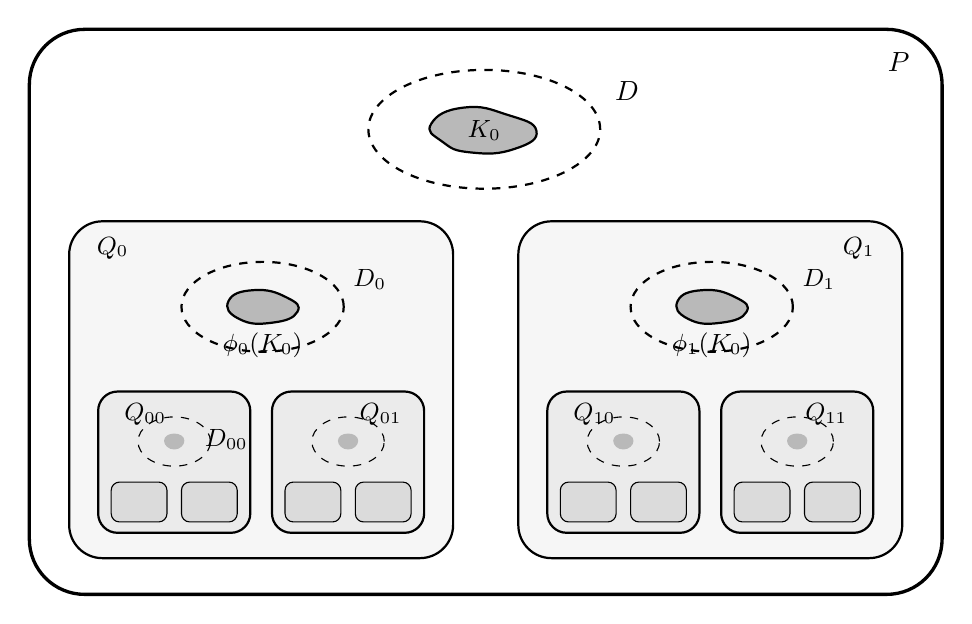
\begin{tikzpicture}[scale=0.92, line join=round, font=\small]
% ---------- the piece P ----------
\draw[very thick, rounded corners=20pt] (0,0) rectangle (12.6,7.8);
\node[font=\normalsize] at (12.0,7.35) {$P$};
% ---------- first-level pullbacks Q_0, Q_1 ----------
\draw[thick, fill=gray!7, rounded corners=12pt] (0.55,0.5) rectangle (5.85,5.15);
\draw[thick, fill=gray!7, rounded corners=12pt] (6.75,0.5) rectangle (12.05,5.15);
\node at (1.15,4.78) {$Q_0$};
\node at (11.45,4.78) {$Q_1$};
% ---------- second-level cylinders inside Q_0 ----------
\draw[thick, fill=gray!16, rounded corners=7pt] (0.95,0.85) rectangle (3.05,2.8);
\draw[thick, fill=gray!16, rounded corners=7pt] (3.35,0.85) rectangle (5.45,2.8);
\node at (1.6,2.48) {$Q_{00}$};
\node at (4.85,2.48) {$Q_{01}$};
% ---------- second-level cylinders inside Q_1 ----------
\draw[thick, fill=gray!16, rounded corners=7pt] (7.15,0.85) rectangle (9.25,2.8);
\draw[thick, fill=gray!16, rounded corners=7pt] (9.55,0.85) rectangle (11.65,2.8);
\node at (7.8,2.48) {$Q_{10}$};
\node at (11.0,2.48) {$Q_{11}$};
% ---------- third-level cylinders (unlabeled) and tiny fibers inside Q_00 ----------
\draw[fill=gray!28, rounded corners=3pt] (1.13,1.0) rectangle (1.9,1.55);
\draw[fill=gray!28, rounded corners=3pt] (2.1,1.0) rectangle (2.87,1.55);
\fill[gray!55] plot [smooth cycle, tension=1] coordinates
  {(1.86,2.12) (2.0,2.22) (2.14,2.12) (2.0,2.0)};
\draw[dashed] (2.0,2.11) ellipse (0.5 and 0.34);
\node at (2.72,2.14) {$D_{00}$};
% ---------- third-level cylinders and tiny fibers inside Q_01 ----------
\draw[fill=gray!28, rounded corners=3pt] (3.53,1.0) rectangle (4.3,1.55);
\draw[fill=gray!28, rounded corners=3pt] (4.5,1.0) rectangle (5.27,1.55);
\fill[gray!55] plot [smooth cycle, tension=1] coordinates
  {(4.26,2.12) (4.4,2.22) (4.54,2.12) (4.4,2.0)};
\draw[dashed] (4.4,2.11) ellipse (0.5 and 0.34);
% ---------- third-level cylinders and tiny fibers inside Q_10 ----------
\draw[fill=gray!28, rounded corners=3pt] (7.33,1.0) rectangle (8.1,1.55);
\draw[fill=gray!28, rounded corners=3pt] (8.3,1.0) rectangle (9.07,1.55);
\fill[gray!55] plot [smooth cycle, tension=1] coordinates
  {(8.06,2.12) (8.2,2.22) (8.34,2.12) (8.2,2.0)};
\draw[dashed] (8.2,2.11) ellipse (0.5 and 0.34);
% ---------- third-level cylinders and tiny fibers inside Q_11 ----------
\draw[fill=gray!28, rounded corners=3pt] (9.73,1.0) rectangle (10.5,1.55);
\draw[fill=gray!28, rounded corners=3pt] (10.7,1.0) rectangle (11.47,1.55);
\fill[gray!55] plot [smooth cycle, tension=1] coordinates
  {(10.46,2.12) (10.6,2.22) (10.74,2.12) (10.6,2.0)};
\draw[dashed] (10.6,2.11) ellipse (0.5 and 0.34);
% ---------- root gap: K_0 and its cell D ----------
\fill[gray!55] plot [smooth cycle, tension=0.9] coordinates
  {(5.55,6.5) (6.0,6.72) (6.6,6.62) (7.0,6.4) (6.7,6.15) (6.1,6.1) (5.7,6.25)};
\draw[thick] plot [smooth cycle, tension=0.9] coordinates
  {(5.55,6.5) (6.0,6.72) (6.6,6.62) (7.0,6.4) (6.7,6.15) (6.1,6.1) (5.7,6.25)};
\node at (6.28,6.4) {$K_0$};
\draw[dashed, thick] (6.28,6.42) ellipse (1.6 and 0.82);
\node[font=\normalsize] at (8.25,6.95) {$D$};
% ---------- level-1 gap of Q_0 ----------
\fill[gray!55] plot [smooth cycle, tension=0.9] coordinates
  {(2.75,4.05) (3.1,4.2) (3.55,4.1) (3.7,3.9) (3.35,3.75) (2.9,3.8)};
\draw[thick] plot [smooth cycle, tension=0.9] coordinates
  {(2.75,4.05) (3.1,4.2) (3.55,4.1) (3.7,3.9) (3.35,3.75) (2.9,3.8)};
\node[below=1pt] at (3.22,3.78) {$\phi_0(K_0)$};
\draw[dashed, thick] (3.22,3.97) ellipse (1.12 and 0.62);
\node at (4.7,4.35) {$D_0$};
% ---------- level-1 gap of Q_1 ----------
\fill[gray!55] plot [smooth cycle, tension=0.9] coordinates
  {(8.95,4.05) (9.3,4.2) (9.75,4.1) (9.9,3.9) (9.55,3.75) (9.1,3.8)};
\draw[thick] plot [smooth cycle, tension=0.9] coordinates
  {(8.95,4.05) (9.3,4.2) (9.75,4.1) (9.9,3.9) (9.55,3.75) (9.1,3.8)};
\node[below=1pt] at (9.42,3.78) {$\phi_1(K_0)$};
\draw[dashed, thick] (9.42,3.97) ellipse (1.12 and 0.62);
\node at (10.9,4.35) {$D_1$};
\end{tikzpicture}
\caption{The direct-decoration gap-cell atlas through depth two.  The
closed Jordan piece $P$ contains the two disjoint closed univalent
pullbacks $Q_0$ and $Q_1$, each of which contains its own next-level
cylinders $Q_{a0},Q_{a1}$, and so on.  The root continuum $K_0$ (blob)
lies in the root gap $P\setminus(Q_0\cup Q_1)$, and the dashed closed
Jordan cell $D$ supplied by Lemma~\ref{lem:jordan-nbhd} isolates it:
$K_0\subset\Int D\subset D\Subset\Int P\setminus(Q_0\cup Q_1)$.  The
inverse branches transport the picture into every cylinder: the fiber
$K_w=\phi_w(K_0)$ lies in the gap of its own cylinder $Q_w$, surrounded
by the dashed cell $D_w=\phi_w(D)\Subset\Int Q_w\setminus(Q_{w0}\cup
Q_{w1})$; the depth-one and depth-two cells $D_0$, $D_1$, $D_{00}$,
$\dots$ are shown.  The cells are pairwise disjoint, including for
ancestor--descendant words, and each one isolates its fiber from the
entire rooted-end compactum: $D_w\cap H_\partial=K_w$
(Theorem~\ref{thm:gap-cells}), so every unselected finite fiber and
every end fiber misses $D_w$.  Dynamics transports the atlas by
$g(D_{aw})=D_w$.}
\label{fig:cells}
\end{figure}

The atlas should be compared clause for clause with
Proposition~\ref{prop:cellwise}: the cells $D_w$ are the pairwise
disjoint closed Jordan disks demanded there, the fibers $K_w$ are the
raw seeds, the fill containment \eqref{eq:F-cell-fill} is the
localization clause, and the exit arcs will be supplied by
Lemma~\ref{lem:impression-port} below.  What the dynamics adds to the
static cellwise picture is the isolation identity
$D_w\cap H_\partial=K_w$, which controls not only the finitely many
packets that a certificate names but \emph{all} fibers of the infinite
compactum at once, and the transport identity $g(D_{aw})=D_w$, which
makes the atlas equivariant.

\subsection{Packet replacement}\label{subsec:F-replacement}

An augmented packet replaces an atom by the filled hull of the atom
together with its protected collars.  In the decoration setting the atoms
are finite fibers, and the replacement must not disturb the connected
complement guaranteed by Theorem~\ref{thm:full-fibers}---otherwise the
free-component criterion of Theorem~\ref{thm:free-component} could fail
after fullification for reasons invisible in the certificate.  The next
theorem rules this out: fullifying finitely many selected fibers inside
their cells leaves the complement connected.

\begin{theorem}[Finite direct-decoration packet replacement; manuscript
Theorem 10.43]\label{thm:packet-replacement}
Let $F\subset\mathcal A^{<\mathbb N}$ be finite and let
\begin{equation}\label{eq:F-replacement}
K_w\subset L_w\Subset\Int D_w,\qquad w\in F,
\end{equation}
with every $L_w$ full (display (DG6) of \cite{MWman}).  Then replacing
the selected fibers $K_w$ by $L_w$ in $H_\partial$, that is, forming
\[
H'
=\Bigl(H_\partial\setminus\bigcup_{w\in F}K_w\Bigr)
\cup\bigcup_{w\in F}L_w ,
\]
gives a compact set with connected sphere complement.
\end{theorem}

\begin{proof}
\emph{The replacement is compact.}
The isolation identity \eqref{eq:F-cell-isolation} makes each selected
$K_w$ clopen in $H_\partial$: it is relatively closed because
$K_w=D_w\cap H_\partial$ with $D_w$ closed, and relatively open because
$K_w=\Int D_w\cap H_\partial$ by \eqref{eq:F-cell-position} and the same
identity.  Hence $H_\partial\setminus\bigcup_{w\in F}K_w$ is a relatively
closed subset of the compact set $H_\partial$, so it is compact, and its
union $H'$ with the finitely many compacta $L_w$ is compact.

\emph{Cells meet deep approximants only in their fibers.}
Fix $w\in F$ and let $m>|w|$.  We claim
\begin{equation}\label{eq:F-cell-approximants}
D_w\cap H_m=K_w ,
\end{equation}
where $H_m$ is the approximant \eqref{eq:F-approximants}.  The inclusion
$\supset$ holds because $K_w$ is a term of $H_m$ (as $|w|<m$) and
$K_w\subset D_w$.  For $\subset$, run the dichotomy of the proof of
Theorem~\ref{thm:gap-cells} over the terms of $H_m$.  A fiber term $K_u$,
$|u|<m$, $u\ne w$: incomparable words have disjoint cylinders; if $u$ is
a strict prefix of $w$ then $D_w\subset Q_{ua}$ for the appropriate child
while \eqref{eq:F-root-gap-pullback} keeps $K_u$ out of both children; if
$w$ is a strict prefix of $u$ then $K_u\subset Q_{wa}$ for some
$a\in\mathcal A$, while $D_w$ misses both children of $Q_w$ by
\eqref{eq:F-cell-position}.  A cylinder term $Q_v$, $|v|=m>|w|$: if $v$
and $w$ are incomparable their cylinders are disjoint; otherwise $w$ is a
strict prefix of $v$, so $Q_v\subset Q_{wa}$ for some $a$, which $D_w$
misses.  This proves \eqref{eq:F-cell-approximants}.

\emph{Modified approximants.}
Put $M=\max_{w\in F}|w|$ and, for $m>M$, make the same replacements in
the approximants:
\[
H_m'
=\Bigl(H_m\setminus\bigcup_{w\in F}K_w\Bigr)
\cup\bigcup_{w\in F}L_w .
\]
Each $H_m'$ is again a finite union of pairwise disjoint full continua.
Indeed, the terms of $H_m$ other than the selected fibers are unchanged,
and each selected term $K_w$ is replaced by the full continuum $L_w$;
disjointness survives because, by \eqref{eq:F-cell-approximants},
\[
L_w\subset\Int D_w
\quad\text{and}\quad
D_w\cap H_m=K_w ,
\]
so $L_w$ meets no unselected term of $H_m$, and distinct selected
replacements $L_w,L_{w'}$ lie in the disjoint cells $D_w,D_{w'}$ of
Theorem~\ref{thm:gap-cells}.  The modified approximants decrease: the
unreplaced parts decrease as in the proof of
Theorem~\ref{thm:full-fibers}, and the replaced terms $L_w$ are constant
in $m$.  Their intersection is the modified rooted-end compactum:
\[
\bigcap_{m>M}H_m'
=\Bigl(\bigcap_{m>M}H_m\setminus\bigcup_{w\in F}K_w\Bigr)
\cup\bigcup_{w\in F}L_w
=H' ,
\]
where the first equality uses \eqref{eq:F-cell-approximants} twice: a
point of $D_w$ lies in $H_m'$ exactly when it lies in $L_w$, and a point
outside every selected cell lies in $H_m'$ exactly when it lies in
$H_m$.

\emph{Conclusion.}
The sets $H_m'$, $m>M$, form a decreasing sequence of compact sets, each
a finite union of pairwise disjoint full continua, with intersection
$H'$.  Lemma~\ref{lem:nested-packets} shows that $\Chat\setminus H'$ is
connected.
\end{proof}

\begin{remark}\label{rem:F-localized}
The proof yields a localized supplement that Theorem~\ref{thm:carrier}
uses.  Fix any Jordan domain $U$ with $P\Subset U$---for instance a
round disk containing $P$.  Every approximant, modified or not, lies in
$P$, hence is compactly contained in $U$, so the localized clause of
Lemma~\ref{lem:nested-packets} applies to the sequence $(H_m')_{m>M}$
and shows that $U\setminus H'$ is connected: the replaced compactum has
one \emph{common} complementary component inside the localization, not
merely a connected complement on the sphere.
\end{remark}

\subsection{Ports at proper protected impressions}\label{subsec:F-port}

The free-component criterion requires each atom to retain a free
singleton port not equal to a protected impression.  In the decoration
setting the atom is a fiber $K_w$, the protected data are finitely many
prime-end crosscut chains, and the port must avoid not only the chains'
collars but the entire fullification of the fiber together with those
collars.  The next lemma produces such a port from a purely metric
selection, under the sole hypothesis that the protected impressions do
not exhaust the boundary.

\begin{lemma}[Proper protected impressions leave a port; manuscript
Lemma 10.44]\label{lem:impression-port}
Let $K\Subset\Int D$ be a nondegenerate full continuum in a closed
Jordan disk $D$, and let $P_{\mathrm{prot}}\subsetneq\partial K$ be
compact.  Then there are a point
$x\in\partial K\setminus P_{\mathrm{prot}}$ and a Jordan arc $\alpha$
from $x$ to $\partial D$, otherwise in $\Int D\setminus K$.  Moreover,
finitely many protected crosscut-chain collars whose impressions have
union contained in $P_{\mathrm{prot}}$ can be truncated so that, for the
connected union $S$ of $K$ with the truncated closed collars,
\begin{equation}\label{eq:F-port}
\alpha\cap\Fill(S)=\{x\}
\end{equation}
(display (DG7) of \cite{MWman}).
\end{lemma}

\begin{proof}
\emph{Metric selection of the port point.}
Since $P_{\mathrm{prot}}$ is a proper compact subset of $\partial K$,
choose $y\in\partial K\setminus P_{\mathrm{prot}}$ and put
$\delta=\dist(y,P_{\mathrm{prot}})>0$ (with $\delta=+\infty$ if
$P_{\mathrm{prot}}=\varnothing$).  Because $y$ is a boundary point of $K$
and $K\Subset\Int D$, every small ball around $y$ contains points of
$\Int D\setminus K$; choose
\[
z\in\Int D\setminus K,\qquad |z-y|<\delta/4 .
\]
Let $x\in K$ minimize the distance to $z$; the minimum is positive since
$z\notin K$ and $K$ is compact.  Every point $p$ of the half-open segment
$(x,z]$ satisfies $|p-z|<|x-z|=\dist(z,K)$, so $(x,z]$ misses $K$; in
particular $x$ is a limit of points of the complement, so
$x\in\partial K$.  The triangle inequality and the minimizing property
(applied against the competitor $y\in K$) give
\[
|x-y|\le|x-z|+|z-y|\le 2|z-y|<\delta/2 ,
\]
hence
$\dist(x,P_{\mathrm{prot}})\ge\delta-|x-y|>\delta/2$ and
$x\notin P_{\mathrm{prot}}$.

\emph{Construction of the arc.}
The complement $\C\setminus K$ of the full continuum is an open connected
subset of the plane, hence arcwise connected \cite{New51}.  Join $z$ by
an arc in $\C\setminus K$ to some point outside $D$, and concatenate
with the segment from $x$ to $z$.  The concatenation is a path from $x$
leaving $D$, contained in $(\C\setminus K)\cup\{x\}$ and meeting $K$ only
at its initial point; extract from it a Jordan arc from $x$ to the far
endpoint, which again meets $K$ only at $x$.  Since the arc starts in
$\Int D$ and ends outside $D$, the parameter set of points on $\partial
D$ is nonempty and closed; truncating at the \emph{first hit} on
$\partial D$ yields a Jordan arc $\alpha$ from $x$ to a point of
$\partial D$ with $\alpha\setminus\{x,\alpha(1)\}\subset\Int D$ and
$\alpha\cap K=\{x\}$.  This proves the first assertion.

\emph{Truncation of the collars.}
Let the finitely many protected chains be
$(\gamma_{j,n},D_{j,n})_{n\ge1}$, prime-end crosscut chains of
$\Chat\setminus K$ whose impressions
$I_j=\bigcap_n\overline{D_{j,n}}$ satisfy
$\bigcup_jI_j\subset P_{\mathrm{prot}}$.  Since $\alpha\cap K=\{x\}$ and
$x\notin P_{\mathrm{prot}}$, the compact sets $\alpha$ and
$P_{\mathrm{prot}}$ are disjoint and have positive distance $2\rho>0$.
Shrinking $\rho$ if necessary, choose for each $j$ an open neighborhood
$W_j$ of $I_j$ contained in the $\rho$-neighborhood of
$P_{\mathrm{prot}}$, in $\Int D$ (possible since
$I_j\subset\partial K\subset K\Subset\Int D$), and in the prescribed
neighborhood of $I_j$ if one was given.  The closures
$\overline{D_{j,n}}$ are nested compact sets with intersection $I_j$, so
for every $j$ there is $n_j$ with
$\overline{D_{j,n_j}}\subset W_j$: otherwise compactness would place a
point of $\bigcap_n\overline{D_{j,n}}=I_j$ outside $W_j$.  Truncate the
$j$-th chain at depth $n_j$ and set
\[
S=K\cup\bigcup_j\overline{D_{j,n_j}} .
\]
Each closed collar meets $K$ in its nonempty impression
$I_j\subset\overline{D_{j,n_j}}\cap K$, so $S$ is a compact connected
set, and $S\Subset\Int D$ by the choice of the $W_j$.  By construction
the truncated collars lie in the $\rho$-neighborhood of
$P_{\mathrm{prot}}$ and therefore miss $\alpha$; hence
\[
\alpha\cap S=\alpha\cap K=\{x\}.
\]

\emph{Extension to infinity and \eqref{eq:F-port}.}
Extend $\alpha$ beyond its endpoint on $\partial D$ by an arc to
$\infty$ in $\C\setminus\Int D$ (for instance, along the image of a
radial ray of the exterior of $D$).  The set
\[
\beta=\alpha\bigl((0,1]\bigr)\cup(\text{the extension})
\]
is connected and unbounded and misses $S$: the extension misses
$S\Subset\Int D$, and $\alpha((0,1])$ misses $S$ by the previous step.
Hence $\beta$ lies in the unbounded component of $\C\setminus S$, and no
point of $\beta$ belongs to $\Fill(S)$, which is $S$ together with the
\emph{bounded} complementary components.  Every point of $\alpha$ except
$x$ lies in $\beta$, and $x\in K\subset S\subset\Fill(S)$; therefore
$\alpha\cap\Fill(S)=\{x\}$, which is \eqref{eq:F-port}.
\end{proof}

\begin{remark}\label{rem:F-collar-confinement}
The proof gives slightly more than the statement: the truncation can
confine the truncated closed collars to any prescribed open
neighborhoods of their impressions, since nested compact crosscut-chain
closures have intersection equal to their impressions and sufficiently
deep tails therefore lie in any such neighborhoods.  This supplement is
established by the proof above, following the manuscript's own proof of
Lemma 10.44; the manuscript's printed statement ends at
\eqref{eq:F-port}, and we use the supplement below with this explicit
attribution.
\end{remark}

\subsection{The protected-carrier theorem}\label{subsec:F-carrier}

The pieces are now assembled.  The theorem below is the finite,
checkable statement toward which the whole paper has been building: at
any fixed decoration depth, any finite selection of fibers, decorated by
actual protected prime-end chains at the root whose impressions do not
exhaust the root boundary, is joined by a protected regulated connector
that respects every piece of the frozen inventory---including the
infinitely many unselected fibers and end fibers.

\begin{theorem}[Finite direct-decoration protected carrier; manuscript
Theorem 10.45]\label{thm:carrier}
Fix a finite set $F\subset\mathcal A^{<\mathbb N}$ of direct-decoration
addresses, and fix finitely many actual protected prime-end crosscut
chains of $\Chat\setminus K_0$ at the root whose total impression is a
proper compact subset of $\partial K_0$.  Then sufficiently deep collar tails of the protected
chains, and the free port supplied by
Lemma~\ref{lem:impression-port}, can be transported through the inverse
branches $\phi_w$, $w\in F$, so that the resulting packet fullifications
remain in the pairwise disjoint cells $D_w$, avoid every unselected
finite fiber and every end fiber, and admit a protected regulated
connector preserving the transported prime ends and their cyclic order.
\end{theorem}

\begin{proof}
\emph{Step 1: root data.}
Discarding duplicates, assume the given chains define pairwise distinct
prime ends: two equivalent chains protect the same access, so nothing is
lost.  Apply Lemma~\ref{lem:impression-port} with $K=K_0$, with $D$ the root
cell of the atlas construction (so $K_0\Subset\Int D$ by
\eqref{eq:F-cell-position} at the empty word), and with
$P_{\mathrm{prot}}$ the union of the impressions of the given protected
chains---a finite union of compacta, compact, and a proper subset of
$\partial K_0$ by hypothesis.  The lemma yields a port point
$x\in\partial K_0\setminus P_{\mathrm{prot}}$, a Jordan arc $\alpha$ from
$x$ to $\partial D$ meeting $K_0$ only at $x$, and truncations of the
protected chains, with closed collar tails in prescribed neighborhoods of
their impressions (Remark~\ref{rem:F-collar-confinement}), such that the
connected union $S$ of $K_0$ with the
truncated closed collars satisfies $S\Subset\Int D$ and
$\alpha\cap\Fill(S)=\{x\}$.  Because the chains define pairwise distinct
prime ends, their deep selected domains are eventually pairwise
disjoint, so after a further truncation---which keeps every conclusion,
the deeper collars being nested in the previous ones---the closed collar
tails may in addition be taken pairwise disjoint, exactly as in the
truncation normalization of Section~\ref{sec:certificates}.  By the fill
containment \eqref{eq:F-cell-fill} applied at the empty word,
\[
\Fill(S)\Subset\Int D .
\]

\emph{Step 2: transport through the inverse branches.}
For $w\in F$ let $\Phi_w\colon\Chat\to\Chat$ be the orientation-preserving
sphere extension of $\phi_w$ constructed in the proof of
Theorem~\ref{thm:full-fibers}.  Define the transported data at address
$w$:
\[
S_w=\Phi_w(S),\qquad
\alpha_w=\Phi_w(\alpha),\qquad
x_w=\phi_w(x),
\]
together with the transported protected chains
$\Phi_w(\gamma_{j,n},D_{j,n})_{n\ge n_j}$.  As in the proof of
Proposition~\ref{prop:naturality}, an orientation-preserving sphere
homeomorphism carries crosscuts of $\Chat\setminus K_0$ to crosscuts of
$\Chat\setminus K_w$, null chains to null chains, selected sides to
selected sides, and preserves the cyclic order of prime ends; so the
transported chains are prime-end crosscut chains of
$\Chat\setminus K_w$, pairwise distinct, with impressions
$\Phi_w(I_j)\subset\partial K_w$, and $S_w$ is the connected union of
$K_w$ with their truncated closed collars.  Fullification commutes with
the transport: $\Phi_w$ maps $\Chat\setminus P$ onto
$\Chat\setminus Q_w$, hence maps the complementary component of $S$
containing $\Chat\setminus P$---the unbounded one---onto the
complementary component of $S_w$ containing $\Chat\setminus Q_w$---again
the unbounded one---and maps the remaining (bounded) complementary
components bijectively onto the remaining ones; therefore
\[
L_w:=\Fill(S_w)=\Phi_w\bigl(\Fill(S)\bigr).
\]
Applying $\Phi_w$ to the Step-1 inclusions and to \eqref{eq:F-port}
gives
\[
K_w\subset L_w\Subset\Int D_w,
\qquad
\alpha_w\cap L_w=\{x_w\},
\]
with $\alpha_w$ a Jordan arc from $x_w$ to $\partial D_w$, otherwise in
$\Int D_w\setminus K_w$.  Each $L_w$ is full: the filled hull of a
continuum is a full continuum.

\emph{Step 3: localization and isolation.}
Theorem~\ref{thm:gap-cells} now localizes and isolates the packets.  The
cells $D_w$, $w\in F$, are pairwise disjoint, so the packet
fullifications $L_w\subset D_w$ are pairwise disjoint and each port arc
$\alpha_w\subset D_w$ meets every other packet's cell not at all.  By the
isolation identity \eqref{eq:F-cell-isolation}, every component of
$H_\partial$ other than $K_w$ misses $D_w$; hence every $L_w$, and every
$\alpha_w$, avoids every unselected finite fiber and every end fiber.

\emph{Step 4: one common free component after fullification.}
The data \eqref{eq:F-replacement} of
Theorem~\ref{thm:packet-replacement} hold for the family
$(L_w)_{w\in F}$, so the replaced compactum
\[
H'=\Bigl(H_\partial\setminus\bigcup_{w\in F}K_w\Bigr)
\cup\bigcup_{w\in F}L_w
\]
is compact with connected sphere complement; and by
Remark~\ref{rem:F-localized}, for a fixed Jordan localization $U$ with
$P\Subset U$ the set $U\setminus H'$ is connected.  Freeze the
inventory of Section~\ref{sec:criterion} as follows: the original atoms
are the selected fibers $K_w$; the closed terminal protected collars are
the truncated collar tails, absorbed into the completed packets $L_w$;
the obstacles are the unselected finite fibers and the end fibers, that
is, $H_\partial\setminus\bigcup_{w\in F}K_w$; the critical-value
exclusion is empty, the branch system \eqref{eq:F-pullbacks} being
univalent; and the localization-forbidden set is $\Chat\setminus U$.
The raw frozen set $Q$ of Section~\ref{sec:criterion} consists of the
listed pieces themselves; the completed packets $L_w$ enlarge the
selected atoms with their truncated collars and the bounded
complementary components added by $\Fill$.  The set $U\setminus H'$ is
connected by Remark~\ref{rem:F-localized}, it lies in
$\Omfree=U\setminus Q$ because $H'\supset Q\cap U$, and it is in fact an
entire component $\Omega_0$ of $\Omfree$: its relative boundary in $U$
lies in $H'$, while the finitely many fill components of the packets
$L_w\setminus S_w$, the only points of $H'$ not in $Q$, are open subsets
of $U\setminus Q$ separate from $U\setminus H'$.  So the component
$\Omega_0=U\setminus H'$ of the frozen free domain contains every port
interior, as the next paragraph verifies.

The port arcs land in it.  Fix $w\in F$.  The cell identity
$D_w\cap H_\partial=K_w$ and the disjointness of the cells give
$D_w\cap H'=L_w$, and $\alpha_w\cap L_w=\{x_w\}=\{\alpha_w(0)\}$; since
$\alpha_w\subset D_w\subset U$, the half-open arc
$\alpha_w((0,1])$ lies in $U\setminus H'=\Omega_0$.  The arcs
$\alpha_w$, $w\in F$, are pairwise disjoint, lying in pairwise disjoint
cells.  Thus $\Omega_0$ has simultaneous singleton ports to every
required atom $K_w$, with each port point $x_w$ a free point not equal
to a protected impression
($x\notin P_{\mathrm{prot}}$ transports to
$x_w\notin\Phi_w(P_{\mathrm{prot}})$).

\emph{Step 5: conclusion by the criterion and the realization theorem.}
By Theorem~\ref{thm:free-component}, the frozen data admit a protected
ribbon-routing certificate: the single free component $\Omega_0$ has
simultaneous singleton ports to every required atom.
Theorem~\ref{thm:realization} realizes the certificate by a compact
connected full carrier that contains every selected fiber $K_w$, has
singleton attachment trace $\{x_w\}$ at each, misses the frozen obstacle
set---in particular every unselected finite fiber and every end
fiber---and preserves every transported protected chain as a prime-end
chain of the enlarged complement, with injective survival and unchanged
cyclic order.  The cyclic order in question is the transported one: by
Step 2 the transport $\Phi_w$ is orientation-preserving and carries the
root cyclic order of the protected chains to the cyclic order at $K_w$,
and Theorem~\ref{thm:realization}(4) preserves the latter.  This is the
asserted protected regulated connector.
\end{proof}

We reproduce the manuscript's caveat, recorded immediately after
Theorem~10.45 of \cite{MWman}, in its own warning environment; the Scope
section returns to it.

\begin{warning}\label{warn:F-finite-scale}
The protected-carrier theorem, Theorem~\ref{thm:carrier}, is finite and
direct-scale only.  It does not construct a second satellite portrait, an
end-fiber return map, a uniform incidence bound, or future fjord, dam,
and attachment data.
\end{warning}

This section is the framework's intended mode of use, and it is worth
stating plainly what has and has not been done.  What has been done is
finite and checkable: at a fixed decoration depth, for an explicitly
listed selection of addresses and an explicitly listed family of
protected root accesses, Theorem~\ref{thm:carrier} produces a protected
regulated connector whose every property---localization in the cells,
isolation from the unselected and end fibers, survival and cyclic order
of the protected prime ends---is certified by the finite data of the
gap-cell atlas and the packet audit, and each such certificate persists
under the monotone operations of Section~\ref{sec:audit}.  What has not
been done is everything infinite or virtual.  The manuscript's open
problems 10.50 (the virtual cylinder target-address selector), 10.51
(disconnected marking transfer to actual bases and iterates on the
cylinders and end fibers of Theorem~\ref{thm:F-compactification}), and
10.52 (virtual Cantor-package realization at every intermediate scale)
are stated as open in \cite{MWman}, remain open, and are not advanced by
anything in this section: no return map on end fibers is constructed, no
end fiber is identified with a small Julia set, and no selection of
target addresses for virtual cylinders is made.  The finite theorem is
offered as what it is---a template showing that, whenever the missing
virtual data are someday supplied, the planar routing they require is
already exact, certified, and persistent.

% ---- end F:decoration ----

% ---- begin F:scope ----
% Cluster F: scope and limitations (Warning 10.59 discipline)
% Body-only LaTeX; preamble macros, theorem environments, and cite keys per CONVENTIONS.md.

\section{Scope and limitations}\label{sec:scope}

The results of this paper form a closed package, and the manuscript
\cite{MWman} disciplines its use with an explicit warning (its
Warning~10.59), whose discipline we retain here in full.  The package has
exactly five load-bearing statements, and their division of labor should
be read precisely.  Theorem~\ref{thm:realization} proves realization
\emph{from} a certificate: given a protected ribbon-routing certificate,
it produces a compact connected full carrier with singleton attachment
traces, surviving protected chains, injective survival, and preserved
cyclic order.  Theorem~\ref{thm:free-component} characterizes \emph{when}
such a certificate exists: exactly when one component of the frozen free
domain has simultaneous singleton ports to every required atom, with the
persistence clause that a separation visible in the frozen data can never
be repaired by monotone connector enlargement.
Theorem~\ref{thm:common-domain} is \emph{one sufficient planar route} to
that criterion: an augmented-atom packet system forces a single common
free component.  Theorem~\ref{thm:audit} removes completion order and
global port untangling from that route: the packet completions are
order-independent, the port checks localize, and merger, localization,
and port-loss defects are persistent certificates of failure.  Finally,
Theorem~\ref{thm:carrier} instantiates the entire package at finite
direct-decoration scale, where the cells of the atlas play the role of
the cellwise data of Proposition~\ref{prop:cellwise} and the nested
packet lemma absorbs the infinitely many unselected fibers.

The mathematical ingredients of all five statements are classical:
Janiszewski's separation theorem and the plane topology of continua
\cite{New51,Why42}, prime ends \cite{Pom92}, filled hulls, and
\v{C}ech cohomology with the compacta form of Alexander duality
\cite{Hat02}, in the tradition of planar arguments long standard in
complex dynamics \cite{DH85}.  The contribution is not a new
theorem about any of these ingredients; it is the assembled
certification framework---explicitly protected accesses with declared
sides, a frozen future inventory fixed before any connector is chosen,
typed packets with order-independent completions, and monotone,
persistent failure certificates.  The paper is proof technology, and its
value is exactly the conversion it performs: informal planar-routing
arguments of the form ``connect these continua while keeping these
accesses and avoiding that set,'' which are traditionally re-derived ad
hoc inside larger proofs, become exact, persistent, checkable
certificates that can be audited clause by clause, transported by
univalent maps, and reused without re-proof.

\begin{warning}\label{warn:F-scope}
Theorem~\ref{thm:realization} proves realization from a certificate.
Theorem~\ref{thm:free-component} characterizes when that certificate
exists, Theorem~\ref{thm:common-domain} proves one sufficient planar
route, and Theorem~\ref{thm:audit} removes completion order and port
untangling from that route.  Theorem~\ref{thm:carrier} instantiates the
package at finite direct-decoration scale, and it is finite and
direct-scale only (Warning~\ref{warn:F-finite-scale}).  None of these
results constructs the virtual Cantor package, the complete Wave
horizon, the analytic covering or immersion maps, a period-independent
incidence bound or future-faithful compression, or any width,
compactness, rigidity, or MLC conclusion.  The
open problems of the source manuscript---10.6, 10.50--10.52, 10.55,
10.57, and 10.58 in the numbering of \cite{MWman}---remain open and are
not advanced here: the virtual canonical interface carrier, the
manuscript's first protected-tower clause, and MLC itself remain open.
\end{warning}

For the reader consulting the manuscript, the open problems named in the
warning are, briefly: 10.6, the virtual protected routing certificate for
the lamination-lift candidate carrier; 10.50, the virtual cylinder
target-address selector; 10.51, the transfer of the disconnected marking
to actual bases and actual iterates on the cylinders and end fibers of
the pullback compactification; 10.52, the virtual Cantor-package
realization at every intermediate scale; and 10.58, the virtual common
free component through the complete Wave horizon, together with the
related problems 10.55 and 10.57.  On the last of these the manuscript is explicit
that neither the connected-hull construction of \cite{Dud25} nor the
primitive-category Hubbard-tree results of \cite{KKL26} supply the
completed free domain that the problem demands; nothing in the present
paper does so either, and nothing here is conditional on those problems:
every theorem above is proved outright in its finite planar setting.

Two further boundaries deserve restatement.  First, the only intentional
divergence from the printed manuscript is the repair of Lemma~10.7 and
the correspondingly rewritten proof of Theorem~10.8, recorded in
Remark~\ref{rem:repair}; every other statement is a faithful
transcription.  Second, no result of this paper asserts local
connectivity of any atom, of any fiber, or of any Julia set, and no
result should be quoted as progress toward MLC.  What may be quoted is
the technology: certificates that realize, criteria that are exact,
audits that are order-free, and one finite dynamical instantiation in
which all of it is checkable.
% ---- end F:scope ----

\section*{Acknowledgments}
The author acknowledges assistance from Fae Build, Anthropic Fable~5, and
OpenAI GPT-5.6 in the preparation of this draft.

\appendix

\section{Crosswalk to the source manuscript}\label{sec:crosswalk}
All results below are reproduced, with notational streamlining and the single
recorded repair, from the source research manuscript~\cite{MWman} (build of
2026-07-27).  No result labelled open or conditional there has been promoted
here.

\begin{center}
\begin{tabular}{lll}
\toprule
Present result & Source manuscript & Note\\
\midrule
Theorem~\ref{thm:no-least} & Theorem 6.12 & verbatim\\
Proposition~\ref{prop:access-collision} & Proposition 6.15 & verbatim\\
Definition~\ref{def:certificate} & Definition 10.1 & verbatim\\
Lemma~\ref{lem:tree-full} & Lemma 10.2 & verbatim\\
Lemma~\ref{lem:crosscut-survival} & Lemma 10.3 & verbatim\\
Theorem~\ref{thm:realization} & Theorem 10.4 & verbatim\\
Proposition~\ref{prop:naturality} & Proposition 10.5 & verbatim\\
Lemma~\ref{lem:slits} & Lemma 10.7 & \emph{repaired; see Remark~\ref{rem:repair}}\\
Theorem~\ref{thm:free-component} & Theorem 10.8 & proof rewritten to the repaired lemma\\
Definition~\ref{def:packet} & Definition 10.9 & verbatim\\
Lemma~\ref{lem:packets} & Lemma 10.10 & verbatim\\
Theorem~\ref{thm:common-domain} & Theorem 10.11 & verbatim\\
Lemma~\ref{lem:fill-absorption} & Lemma 10.12 & verbatim\\
Lemma~\ref{lem:port-localization} & Lemma 10.13 & verbatim\\
Theorem~\ref{thm:audit} & Theorem 10.14 & verbatim\\
Proposition~\ref{prop:cellwise} & Proposition 10.15 & verbatim\\
Lemma~\ref{lem:nested-packets} & Lemma 10.39 & verbatim\\
Theorem~\ref{thm:full-fibers} & Theorem 10.40 & verbatim\\
Lemma~\ref{lem:jordan-nbhd} & Lemma 10.41 & verbatim\\
Theorem~\ref{thm:gap-cells} & Theorem 10.42 & verbatim\\
Theorem~\ref{thm:packet-replacement} & Theorem 10.43 & verbatim\\
Lemma~\ref{lem:impression-port} & Lemma 10.44 & verbatim\\
Theorem~\ref{thm:carrier} & Theorem 10.45 & verbatim\\
\bottomrule
\end{tabular}
\end{center}

The examples of Sections~\ref{sec:criterion} and~\ref{sec:audit}
(Examples~\ref{ex:no-common-component} and~\ref{ex:merger}) and the
comparison Section~\ref{sec:comparison} are new expository material added for
this paper; they promote no manuscript claim.

\begin{thebibliography}{99}

\bibitem{DH85}
A.~Douady and J.~H.~Hubbard,
\emph{On the dynamics of polynomial-like mappings},
Ann. Sci. \'Ec. Norm. Sup\'er. (4) \textbf{18} (1985), 287--343.

\bibitem{Dud25}
D.~Dudko,
\emph{Local connectivity of the Mandelbrot set: a roadmap},
ICM 2026 survey, arXiv:2512.24171, 2025.

\bibitem{Hat02}
A.~Hatcher,
\emph{Algebraic Topology},
Cambridge University Press, 2002.

\bibitem{KKL26}
J.~Kahn, A.~Kapiamba, and M.~Lyubich,
\emph{MLC for parabolically bounded primitive renormalization},
arXiv:2606.27272, 2026.

\bibitem{KL08}
J.~Kahn and M.~Lyubich,
\emph{A priori bounds for some infinitely renormalizable quadratics. II. Decorations},
Ann. Sci. \'Ec. Norm. Sup\'er. (4) \textbf{41} (2008), 57--84.

\bibitem{Moo25}
R.~L.~Moore,
\emph{Concerning upper semi-continuous collections of continua},
Trans. Amer. Math. Soc. \textbf{27} (1925), 416--428.

\bibitem{MWman}
M.~R.~Wesney,
\emph{A marked-width reduction of Mandelbrot local connectivity},
research manuscript, 2026 (build of 2026-07-27).

\bibitem{New51}
M.~H.~A.~Newman,
\emph{Elements of the Topology of Plane Sets of Points},
2nd ed., Cambridge University Press, 1951.

\bibitem{Pom92}
Ch.~Pommerenke,
\emph{Boundary Behaviour of Conformal Maps},
Grundlehren der mathematischen Wissenschaften \textbf{299},
Springer-Verlag, 1992.

\bibitem{Why42}
G.~T.~Whyburn,
\emph{Analytic Topology},
AMS Colloquium Publications \textbf{28},
American Mathematical Society, 1942.

\end{thebibliography}

\end{document}
